%!TEX program = xelatex
%!TEX options=--shell-escape
\documentclass[12pt]{article}

%
\usepackage[scheme=plain]{ctex}
%
\usepackage{fontspec}
%
\usepackage[margin = 1in]{geometry}

%
\usepackage[dvipsnames]{xcolor}
\usepackage[many]{tcolorbox}

%
\usepackage{amsmath}
\usepackage{amssymb}
\usepackage{amsthm}
%
\usepackage{tensor}
%
\usepackage{slashed}
\usepackage{physics}
\usepackage{simpler-wick}

%
\usepackage[version=4]{mhchem}

%
\usepackage{mathtools}

%
\usepackage{bm}
\newcommand{\dbar}{\dif\hspace*{-0.18em}\bar{}\hspace*{0.2em}}
\DeclareMathAlphabet\mathbfcal{OMS}{cmsy}{b}{n}
%\usepackage{bbold}
\newcommand*{\dif}{\mathop{}\!\mathrm{d}}
\newcommand*{\euler}{\mathrm{e}}
\newcommand*{\imagi}{\mathrm{i}}

\renewcommand{\vec}[1]{\boldsymbol{\mathbf{#1}}}

\usepackage{caption}
\usepackage{multirow}
\usepackage{enumitem}

%
\usepackage{mathrsfs}
\usepackage{dsfont}

%
\usepackage{hyperref}
\hypersetup{
    colorlinks=true,
    linkcolor=violet,
    filecolor=blue,
    urlcolor=blue,
    citecolor=cyan,
}

%
\usepackage{graphicx}
\usepackage{subfig}
%
\graphicspath{{figures/}{../figures/}}


%
\usepackage{indentfirst}
%
\setlength{\parindent}{2em}
\linespread{1.25}

%
% \setmainfont{Times New Roman}

\title{Note}
\author{Feng-Yang Hsieh}
\date{}

\begin{document}
\maketitle

\section{CWoLa}% (fold)
\label{sec:cwola}
    The Classification Without Labels (CWoLa) is a weakly supervised learning method. The CWoLa approach trains a model to discriminate the mixed samples, which are mixtures of the original signal and background samples. The optimal classifier in the CWoLa approach is also the optimal classifier in the traditional fully supervised case where all label information is available. This section utilizes the CWoLa approach to train classifiers on di-Higgs samples.

    \subsection{Sample}% (fold)
    \label{sub:sample}
        This exercise's signal corresponds to the resonant Higgs boson pairs production in the four-$b$ quarks channel. These Higgs boson pairs are produced via gluon-gluon fusion in the two Higgs doublet model (2HDM). The Higgs boson $h$ ($m_h = \text{125 GeV}$) pair is produced by the heavy CP-even scalar $H$ with mass $m_H$ ranging from $\text{300 GeV}$ to $\text{1200 GeV}$. The background consists of QCD multi-jet events.

        The CWoLa training samples $M_1$ and $M_2$ are the mixtures of the signal and background samples. The probability distribution of the mixed sample is a combination of the signal $p_s(x)$ and background $p_B(x)$ distributions:
        \begin{equation}
            \begin{aligned}
                p_{M_1}(x) &=  f_1 p_S(x) + (1-f_1) p_B(x) \\
                p_{M_2}(x) &=  f_2 p_S(x) + (1-f_2) p_B(x)
            \end{aligned}
        \end{equation}
        where $f_1, f_2$ are the signal fractions, and $x$ represents the observables used for the classification task.

        DNN and SPANet network architectures are considered in this exercise. For DNN, the input features are summarised in Table \ref{tab:DNN_variables}, consisting of 16 variables. For SPANet, the input features are a list of final jets, each represented by their 4-momentum $(p_\text{T}, \eta,\phi, M)$ and a boolean $b$-tag.
        \begin{table}[htpb]
            \centering
            \caption{Input variables used to train the dense neural network.}
            \label{tab:DNN_variables}
            \begin{tabular}{l|c|c}
                Reconstructed objects       & Variables used for training   & \# \\ \hline
                Higgs candidate             & $(p_\text{T}, \eta, \phi, m)$ & 8  \\
                Subjets                     & $\Delta R(j_1,j_2)$                    & 2  \\
                b-tagging                   & Boolean for $j_i \in h_{1,2}^{\text{cand}}$       & 4  \\
                Di-Higgs system             & $p_\text{T}^{hh}, m_{hh}$        & 2
            \end{tabular}
        \end{table}

    % subsection sample (end)
    \subsection{Result}% (fold)
    \label{sub:result}
        The CWoLa training utilizes samples with different signal fractions $f_1,f_2$ to train the classifiers. The results of CWoLa training are shown in Figure~\ref{fig:CWoLa_training_result} with different signal fractions. When $f_1$ is far from $0.5$, the results tend to approach those of the fully supervised case.
        \begin{figure}[htpb]
            \centering
            \subfloat[DNN]{
                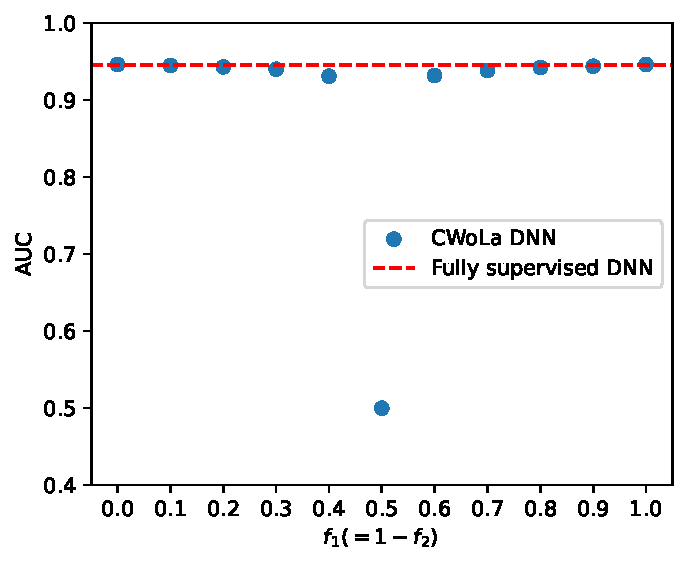
\includegraphics[width=0.45\textwidth]{CWoLa_DNN.pdf}
            }
            \subfloat[SPANet]{
                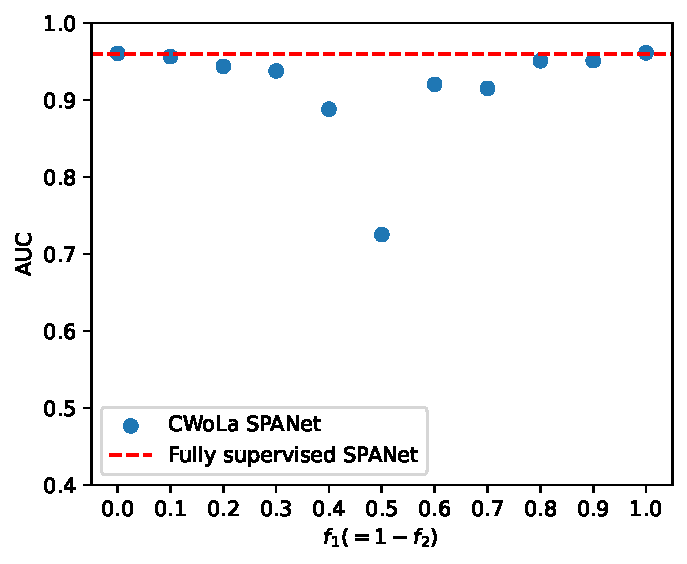
\includegraphics[width=0.45\textwidth]{CWoLa_SPANet.pdf}
            }
            \caption{The AUC of CWoLa training as a function of the signal fraction $f_1$. For simplicity, we set signal fraction $f_2$ equal to $1 - f_1$. The horizontal dashed line indicates the fully-supervised AUC.}
            \label{fig:CWoLa_training_result}
        \end{figure}

        When $f_1 = 0.5$ the mixed sample $M_1$ and $M_2$ have identical distributions, so the classifier can not learn anything in this case. In the case of DNN, the AUC is $0.5$, as expected. However, for SPANet, the AUC is more than $0.7$.

        This is because SPANet is trained on both pairing and classification tasks simultaneously. The pairing part introduces asymmetries between signal and background samples, leading to the AUC that deviates from $0.5$.

        To investigate the effect of the pairing task on SPANet's performance, the weight of the pairing component is set to zero, meaning that SPANet focuses solely on the classification task. Figure~\ref{fig:CWoLa_SPANet_without_pairing} shows the SPANet training results without pairing task. As expected, the AUC is close to $0.5$ when $f_1 = 0.5$.
        \begin{figure}[htpb]
            \centering
            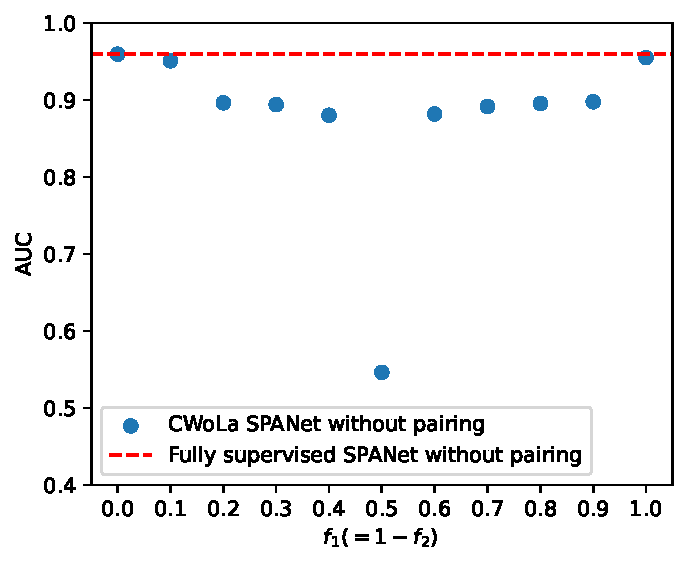
\includegraphics[width=0.65\textwidth]{CWoLa_SPANet_no_pair.pdf}
            \caption{The AUC of CWoLa SPANet training as a function of the signal fraction $f_1$. For simplicity, we set signal fraction $f_2$ equal to $1 - f_1$. Here, SPANet is trained on the classification task only.}
            \label{fig:CWoLa_SPANet_without_pairing}
        \end{figure}
    % subsection result (end)
% section cwola (end)

\section{CWoLa hunting}% (fold)
\label{sec:cwola_hunting}
    The CWoLa hunting approach considers a $m_{\text{res}}$ variable. For background, the $m_{\text{res}}$ distribution is smooth while signal $m_{\text{res}}$ distribution is expected to be localized near some $m_0$. Consequently, this variable could be used to create two mixed samples. Additional features that are uncorrelated with $m_{\text{res}}$ can be used for training a classifier. This technic is first introduced by Reference~\cite{Collins:2018epr}.
    \subsection{Sample}% (fold)
    \label{sub:sample_cwola_hunting}
        The signal is the resonant Higgs boson pairs production in the four-$b$ quarks channel. This section produces the Higgs boson pair by the heavy CP-even scalar $H$ with mass $m_H = \text{500 GeV}$ or $m_H = \text{1000 GeV}$. The background consists of QCD multi-jet events. The basic requirement is the ``four-tag cut,'' which requires at least four $b$-tagged $R = 0.4$ anti-$k_t$ jets with $p_\text{T} > \text{40 GeV}$ and $\abs{\eta} < 2.5$. Only the events passing the four-tag cut are used in the following analysis.

        The CWoLa hunting approach utilizes the signal and sideband regions to create the mixed training sample. The di-Higgs system's total invariant mass $m_{hh}$ determines the signal and sideband region. This quantity is computed from the four $b$-jets with the highest transverse momentum. Figure~\ref{fig:mhh_distribution} presents the $m_{hh}$ distribution of signal and background samples. Table~\ref{tab:signal_sideband_range} summarizes the signal and sideband regions. These signal and sideband regions are chosen such that the corresponding cross-sections are closed.
        \begin{figure}[htpb]
            \centering
            \subfloat[$m_H = \text{500 GeV}$]{
                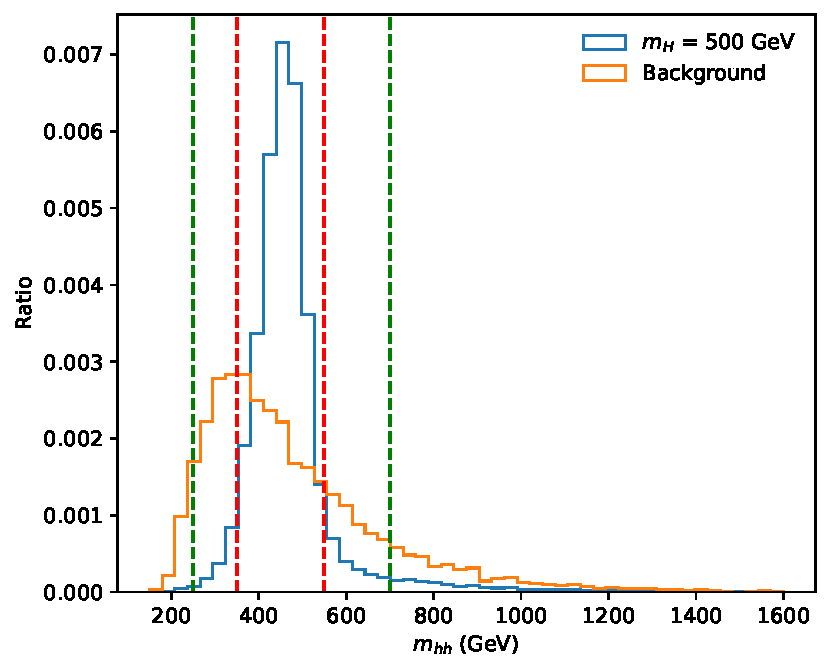
\includegraphics[width=0.45\textwidth]{mhh_distribution-500GeV.pdf}
            }
            \subfloat[$m_H = \text{1000 GeV}$]{
                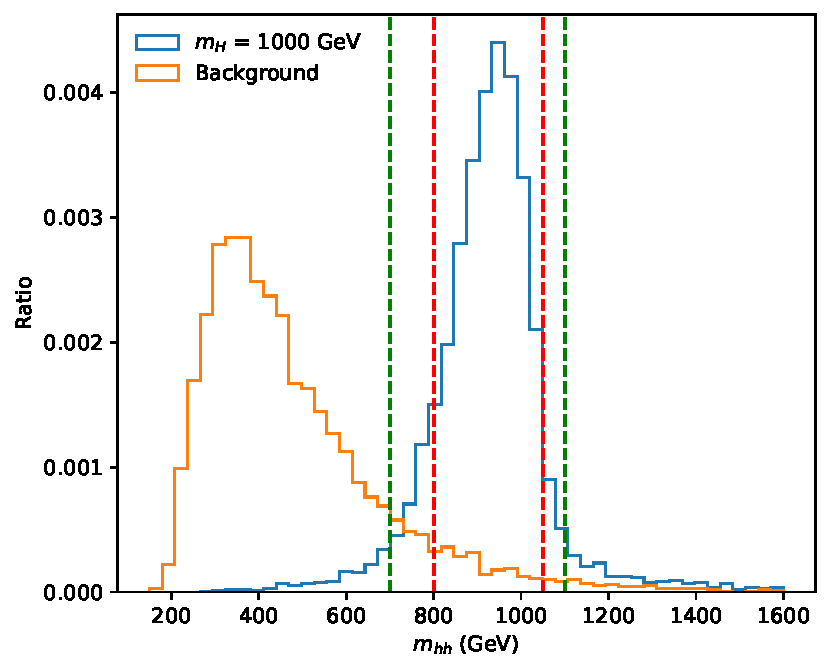
\includegraphics[width=0.45\textwidth]{mhh_distribution-1000GeV.pdf}
            }
            \caption{The total invariant mass $m_{hh}$ distribution of signal and background samples. The signal region is between the red dashed lines. The sideband region is between the green dashed lines and excludes the signal region.}
            \label{fig:mhh_distribution}
        \end{figure}

        \begin{table}[htpb]
            \centering
            \caption{The signal and sideband regions with different resonant samples. The unit is GeV.}
            \label{tab:signal_sideband_range}
            \begin{tabular}{r|cc}
                $m_H$ & Signal       & Sideband                      \\ \hline
                500   & $[350, 550]$ & $[250, 350]\cup [550, 700]$   \\
                1000  & $[800,1050]$ & $[700, 800]\cup [1050, 1100]$
            \end{tabular}
        \end{table}
        Table~\ref{tab:diHiggs_cutflow_table} is the cutflow table of the selection cuts. The number of events used in mixed training samples could be computed from these cross-sections. The training sample size is presented in Table~\ref{tab:training_sample_size_cwola_hunting}.
        \begin{table}[htpb]
            \centering
            \caption{The cross sections for the di-Higgs signal and background processes at different selection cuts.}
            \label{tab:diHiggs_cutflow_table}
            \begin{tabular}{c|l|cc|c|c}
                                      &                 & \multicolumn{2}{c|}{Cross section (fb)} &          & $\mathcal{L} = 139 \text{ fb}^{-1}$ \\
                $m_H$ (GeV)           &                 & Signal           & Background           & $S / B$  & $S/\sqrt{B}$                        \\ \hline
                \multirow{3}{*}{500}  & Four tag        & 3.64             & 6.03e+03             & 6.03e-04 & 0.553                               \\ \cline{2-6}
                                      & Signal region   & 3.13             & 2.57e+03             & 1.22e-03 & 0.727                               \\
                                      & Sideband region & 0.35             & 2.36e+03             & 1.50e-04 & 0.086                               \\ \hline \hline
                \multirow{3}{*}{1000} & Four tag        & 0.081            & 6.03e+03             & 1.34e-05 & 0.0123                              \\ \cline{2-6}
                                      & Signal region   & 0.063            & 3.32e+02             & 1.90e-04 & 0.0408                              \\
                                      & Sideband region & 0.010            & 3.19e+02             & 3.03e-05 & 0.0064
            \end{tabular}
        \end{table}

        \begin{table}[htpb]
            \centering
            \caption{The training sample size for the mixed sample. The luminosity is $\mathcal{L} = 78 \text{ fb}^{-1}$ because the generated samples are not enough for now.}
            \label{tab:training_sample_size_cwola_hunting}
            \begin{tabular}{c|c|cc}
                                      &              & \multicolumn{2}{c}{True label} \\
                $m_H$ (GeV)           & Mixed sample & Signal       & Background      \\ \hline
                \multirow{2}{*}{500}  & $M_1$        & 244          & 200k            \\
                                      & $M_2$        & 28           & 184k            \\ \hline
                \multirow{2}{*}{1000} & $M_1$        & 5            & 26k             \\
                                      & $M_2$        & 1            & 25k
            \end{tabular}
        \end{table}

        Consider the DNN CWoLa classifier. The Higgs candidates are reconstructed by the $\text{min-}\Delta R$ pairing method. In the $\text{min-}\Delta R$ method, the four $b$-tagged jets with the highest $p_{\text{T}}$ are used to form the two Higgs boson candidates. The $\text{min-}\Delta R$ method selects the pairing configuration in which the higher-$p_{\text{T}}$ jet pair has the smallest $\Delta R$ separation. The input features are similar to the previous case (Table~\ref{tab:DNN_variables}), but the $b$-tagging information and the di-Higgs system's total invariant mass are excluded. $\text{min-}\Delta R$ pairing only uses the $b$-tagged jets. Total invariant mass is already used to determine the signal and sideband region.

    % subsection sample_cwola_hunting (end)
    \subsection{Training results}% (fold)
    \label{sub:training_results}
        Table \ref{tab:cwola_hunting_DNN_results} presents the DNN classification training results. These numbers are evaluated from the pure samples, which consist of 5k signal events and 5k background events. The training datasets with and without signal events have similar results. This suggests that the DNN fails to distinguish the signal and background samples but learns the difference between the signal and sideband region. Moreover, the results also imply the input features may correlate to the total invariant mass of the di-Higgs system.
        \begin{table}[htpb]
            \centering
            \caption{The CWoLa DNN training results. ACC is the best accuracy and AUC is the area under the ROC curve. The average and standard deviation of 10 training are presented.}
            \label{tab:cwola_hunting_DNN_results}
            \begin{tabular}{c|c|cc}
                $m_H$ (GeV)           &             & ACC               & AUC               \\ \hline
                \multirow{2}{*}{500}  & With signal & $0.708 \pm 0.002$ & $0.770 \pm 0.007$ \\
                                      & No signal   & $0.705 \pm 0.003$ & $0.769 \pm 0.009$ \\ \hline
                \multirow{2}{*}{1000} & With signal & $0.868 \pm 0.024$ & $0.925 \pm 0.023$ \\
                                      & No signal   & $0.850 \pm 0.033$ & $0.909 \pm 0.026$
            \end{tabular}
        \end{table}

        Figure~\ref{fig:signal_score_distribution} shows the signal score distributions. Even though the signal scores are very different for signal and background distributions, the difference probably stems from the $m_{hh}$ distribution.
        \begin{figure}[htpb]
            \centering
            \subfloat[$m_H = \text{500 GeV}$]{
                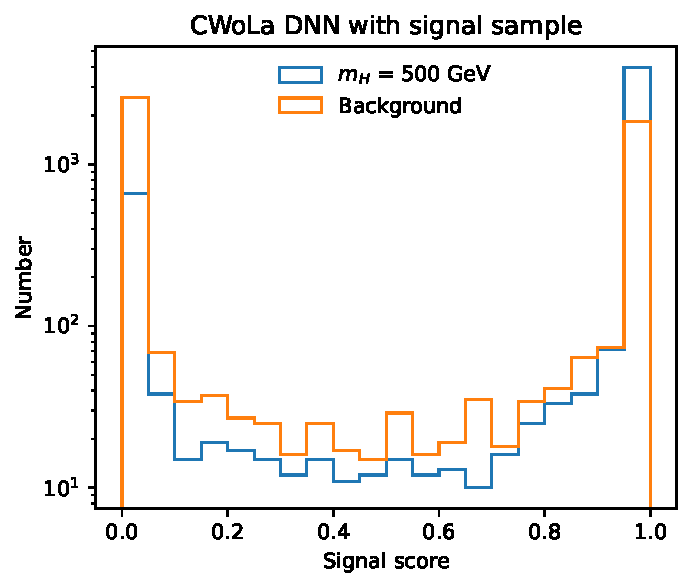
\includegraphics[width=0.45\textwidth]{DNN_w_sig_signal_score_distribution-500GeV.pdf}
                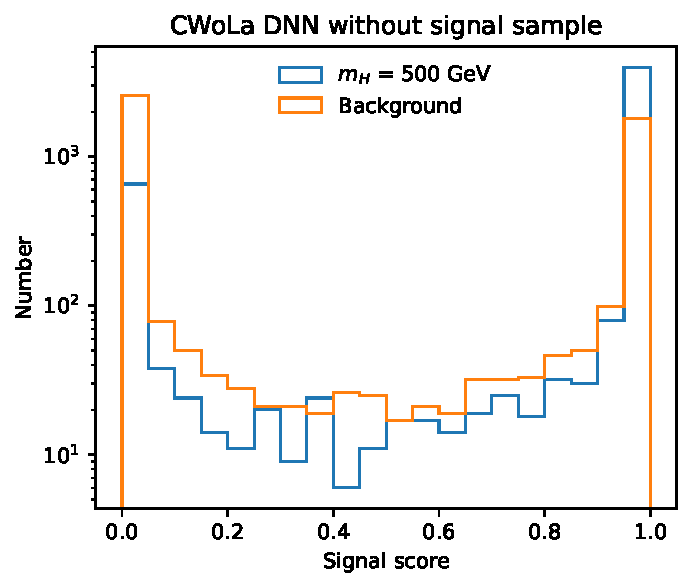
\includegraphics[width=0.45\textwidth]{DNN_wo_sig_signal_score_distribution-500GeV.pdf}
            }
            \\
            \subfloat[$m_H = \text{1000 GeV}$]{
                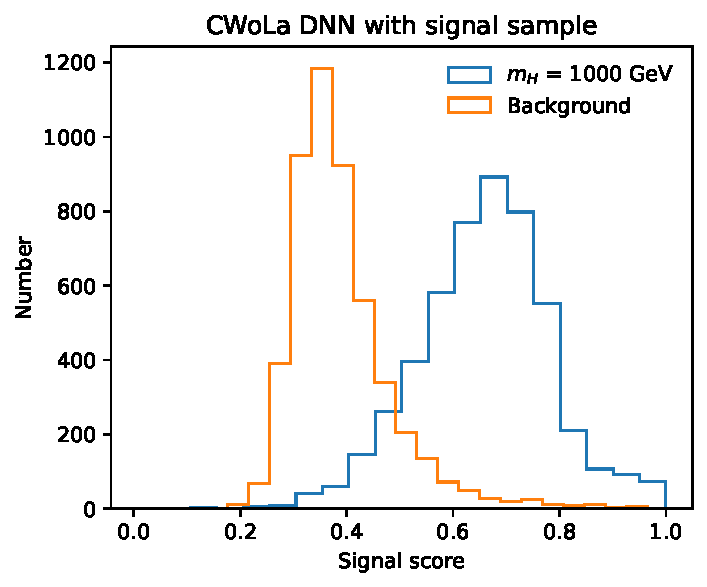
\includegraphics[width=0.45\textwidth]{DNN_w_sig_signal_score_distribution-1000GeV.pdf}
                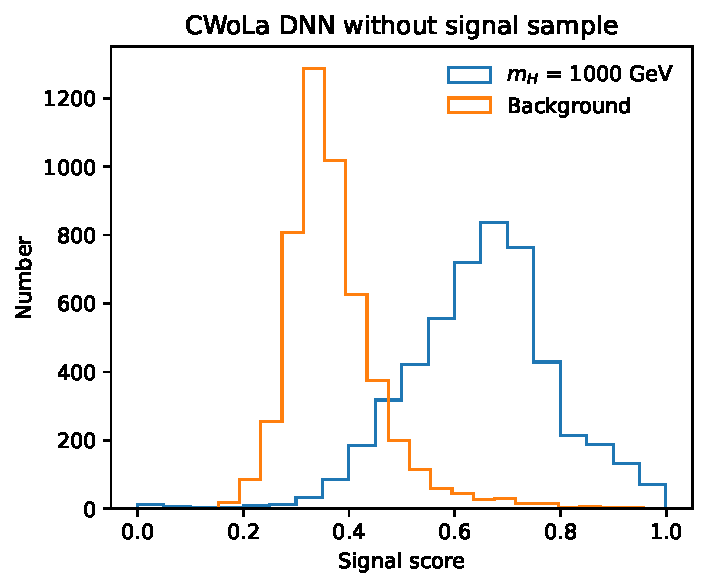
\includegraphics[width=0.45\textwidth]{DNN_wo_sig_signal_score_distribution-1000GeV.pdf}
            }
            \caption{The signal score distributions. We apply the CWoLa DNN on pure samples to obtain the signal score distributions.}
            \label{fig:signal_score_distribution}
        \end{figure}

        There are two issues:
        \begin{itemize}
            \item The input features might correlated to the observables used to determine the signal and sideband region. We need to construct other independent input variables.
            \item The signal fraction is too low. It is hard to learn something about signal events.
        \end{itemize}
    % subsection training_results (end)
    \subsection{Correlation matrix}% (fold)
    \label{sub:correlation_matrix}
        The results in Section~\ref{sub:training_results} imply that the di-Higgs system's total invariant mass is not independent of other input features. To find the variables that are highly dependent on the total invariant mass, the correlation coefficients are computed among these variables. Figure~\ref{fig:correlation_coefficient_500GeV} and \ref{fig:correlation_coefficient_1000GeV} are correlation coefficients on the $\text{500 GeV}$ and $\text{1000 GeV}$ cases, respectively.

        \begin{figure}[htpb]
            \centering
            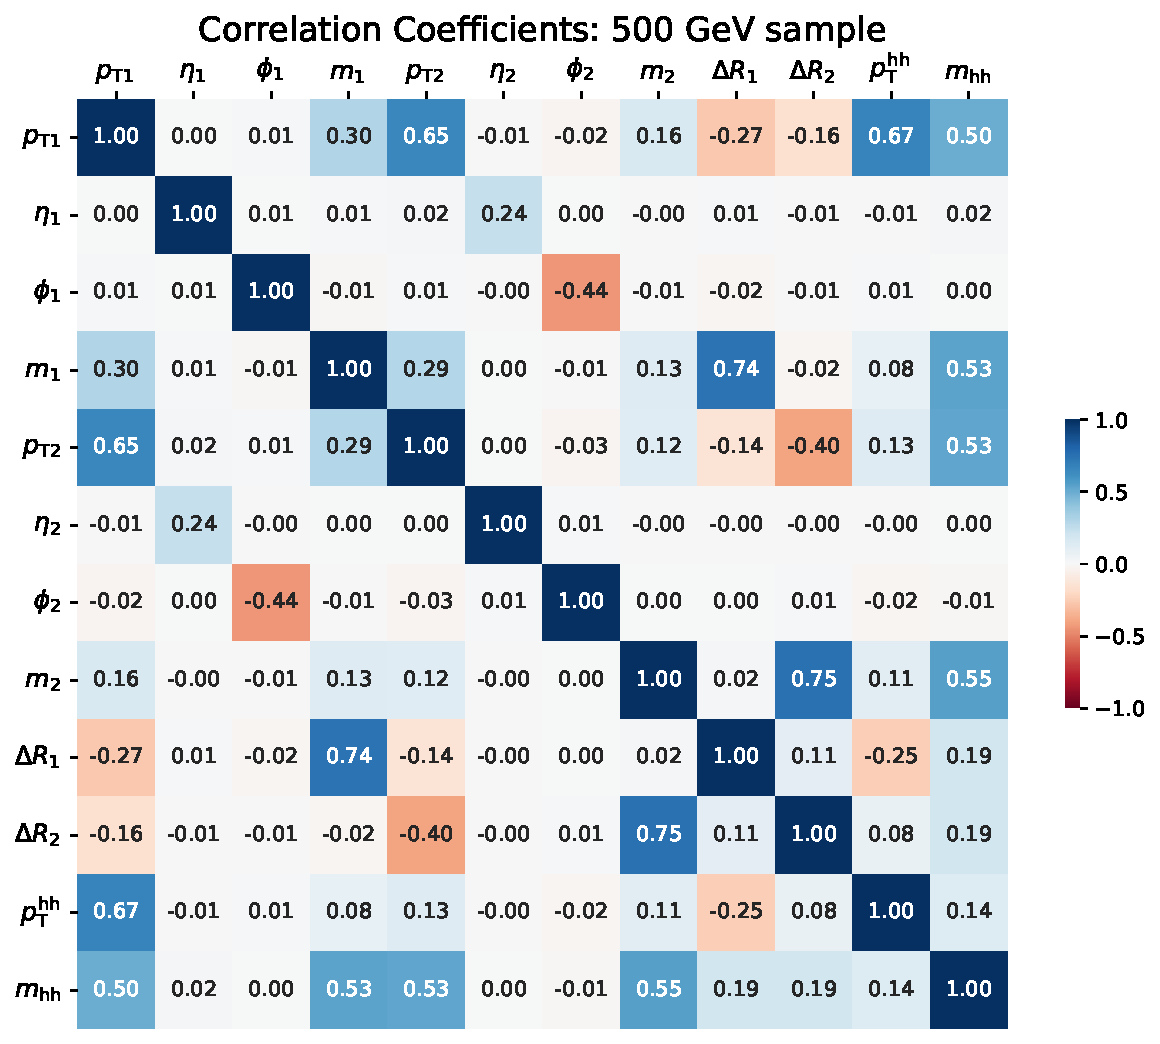
\includegraphics[width=0.9\textwidth]{correlation_coefficients-500GeV.pdf}
            \caption{The correlation coefficients among different variables are computed from $\text{500 GeV}$ testing sample, consisting of 5k signal and 5k background.}
            \label{fig:correlation_coefficient_500GeV}
        \end{figure}

        \begin{figure}[htpb]
            \centering
            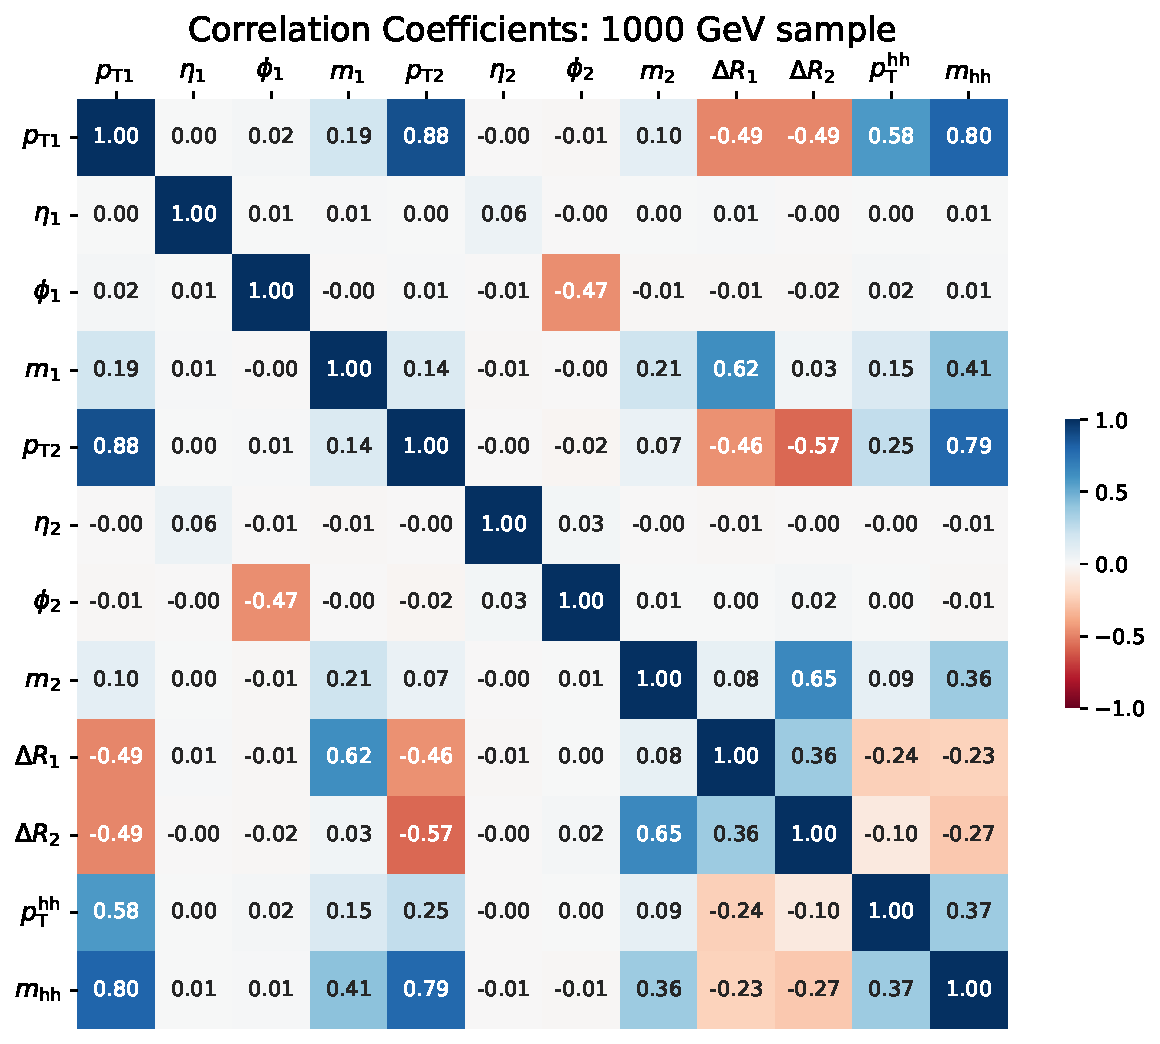
\includegraphics[width=0.9\textwidth]{correlation_coefficients-1000GeV.pdf}
            \caption{The correlation coefficients among different variables are computed from $\text{1000 GeV}$ testing sample, consisting of 5k signal and 5k background.}
            \label{fig:correlation_coefficient_1000GeV}
        \end{figure}

        The results show that the transverse momentum $p_\text{T}$ and the invariant mass $m$ of Higgs candidates are highly correlated to the total invariant mass. Figure~\ref{fig:pt1_mhh_scatter_plot} shows the scatter plots of the transverse momentum of the leading Higgs candidate and the total invariant mass $m_{\text{hh}}$. These plots also explain why the DNN only trained on background samples can distinguish the signal and background events, because the background distribution in the signal and sideband regions are different.
        \begin{figure}[htpb]
            \centering
            \subfloat[$m_H = \text{500 GeV}$]{
                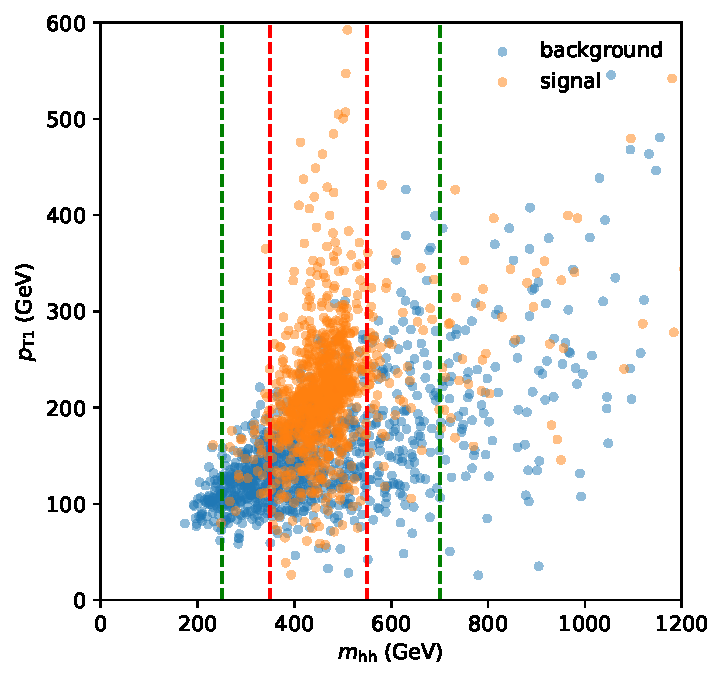
\includegraphics[width=0.45\textwidth]{scatter_plot_mhh_pt1-500GeV.pdf}
            }
            \subfloat[$m_H = \text{1000 GeV}$]{
                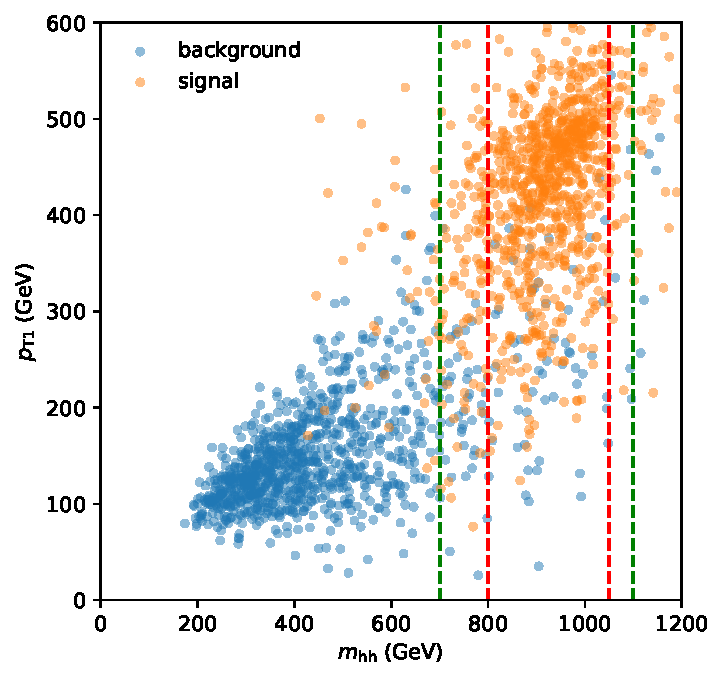
\includegraphics[width=0.45\textwidth]{scatter_plot_mhh_pt1-1000GeV.pdf}
            }
            \caption{The scatter plots of the transverse momentum of leading Higgs candidate $p_{\text{T}1}$ and total invariant mass $m_{hh}$ distribution. The signal region is between the red dashed lines. The sideband region is between the green dashed lines and excludes the signal region.}
            \label{fig:pt1_mhh_scatter_plot}
        \end{figure}
    % subsection correlation_matrix (end)
    \subsection{Remove highly correlated features}% (fold)
    \label{sub:remove_highly_correlated_features}
         Figure~\ref{fig:correlation_coefficient_500GeV} and \ref{fig:correlation_coefficient_1000GeV} show that the transverse momentum $p_\text{T}$ and the invariant mass $m$ of Higgs candidates are highly related to the total invariant mass $m_{hh}$. To investigate the impact of these highly correlated features on the discrimination power of CWoLa DNN models, we remove these input features and train the DNN model again.

        \begin{table}[htpb]
            \centering
            \caption{The CWoLa DNN training results. The transverse momentum and invariant mass of Higgs candidates are removed from samples. ACC is the best accuracy and AUC is the area under the ROC curve. The average and standard deviation of 10 training are presented.}
            \label{tab:cwola_hunting_DNN_results_wo_pt_m}
            \begin{tabular}{c|c|cc}
                $m_H$ (GeV)           &             & ACC               & AUC               \\ \hline
                \multirow{2}{*}{500}  & With signal & $0.526 \pm 0.020$ & $0.536 \pm 0.053$ \\
                                      & No signal   & $0.532 \pm 0.015$ & $0.543 \pm 0.029$ \\ \hline
                \multirow{2}{*}{1000} & With signal & $0.586 \pm 0.030$ & $0.625 \pm 0.046$ \\
                                      & No signal   & $0.564 \pm 0.024$ & $0.583 \pm 0.042$
            \end{tabular}
        \end{table}

         Table~\ref{tab:cwola_hunting_DNN_results_wo_pt_m} summarizes the results of the CWoLa DNN training without $p_{\text{T}}$ and $m$ features. The training datasets with and without signal events still have similar results. Compared to the previous one (Table~\ref{tab:cwola_hunting_DNN_results}) the accuracy values are closer to 0.5. These results suggest that the removed features significantly contribute to the model's discrimination power, and the remaining parameters are hard to utilize to distinguish the signal and background events.
    % subsection remove_highly_correlated_features (end)
    \subsection{Transverse momentum cut testing}% (fold)
    \label{sub:pt_cut_testing}
        In Figure~\ref{fig:mhh_distribution}, the distribution of the background sample exhibits a gradual termination around $\text{150 GeV}$. To investigate whether this termination is a result of the ``four-tag cut'', which requires $p_{\text{T}} > \text{40 GeV}$, total invariant mass distributions with different $p_{\text{T}}$ cuts are plotted in Figure~\ref{fig:mhh_distribution_bkg_pt}. As the transverse momentum requirement increases from $\text{40 GeV}$ to $\text{70 GeV}$, the termination point also shifts to larger values. Moreover, the termination remains gradual rather than an abrupt cut-off, suggesting that the gradual termination indeed results from the transverse momentum cut.
        \begin{figure}[htpb]
            \centering
            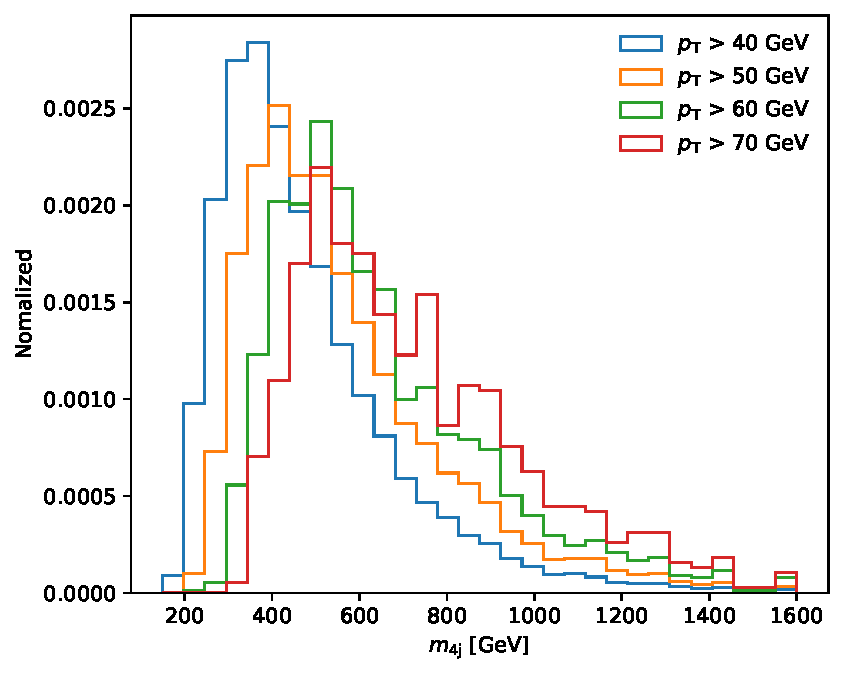
\includegraphics[width=0.5\textwidth]{m4j_distribution_background_various_pt_cut.pdf}
            \caption{The total invariant mass $m_{\text{4j}}$ distribution of background samples. The transverse momentum requirement varies from $\text{40 GeV}$ to $\text{70 GeV}$.}
            \label{fig:mhh_distribution_bkg_pt}
        \end{figure}
    % subsection pt_cut_testing (end)
    \subsection{Enlarge the signal sample size}% (fold)
    \label{sub:enlarge_the_signal_sample_size}
        Another issue arises from the low signal fraction (Table~\ref{tab:training_sample_size_cwola_hunting}), making DNN difficult to extract meaningful information about signal events. To investigate the impact of signal sample size, we increase the signal size manually and retrain the DNN model. The training sample sizes are summarized in Table~\ref{tab:training_sample_size_cwola_hunting_enlarge_signal_size}.

        \begin{table}[htpb]
            \centering
            \caption{The training sample size for the mixed sample. Various signal sizes are considered, and the background sizes are fixed for all cases. ``1 times'' represents the previous ``With signal'' case and ``0 times'' represents the previous ``No signal'' case.}
            \label{tab:training_sample_size_cwola_hunting_enlarge_signal_size}
            \begin{tabular}{c|c|cccc|c}
                                      &              & \multicolumn{4}{c|}{Signal}              & Background \\ \hline
                $m_H$ (GeV)           & Mixed sample & 1 times & 0 times & 10 times & 100 times & All        \\ \hline
                \multirow{2}{*}{500}  & $M_1$        & 244     & 0       & 2438     & 24380     & 200k       \\
                                      & $M_2$        & 28      & 0       & 276      & 2760      & 184k       \\ \hline
                \multirow{2}{*}{1000} & $M_1$        & 5       & 0       & 49       & 492       & 26k        \\
                                      & $M_2$        & 1       & 0       & 8        & 75        & 25k
            \end{tabular}
        \end{table}

        \begin{table}[htpb]
            \centering
            \caption{The CWoLa DNN training results. The transverse momentum and invariant mass of Higgs candidates are removed from samples. 1 time and 0 times are the with signal and no signal case in Table~\ref{tab:cwola_hunting_DNN_results_wo_pt_m}. ACC is the best accuracy and AUC is the area under the ROC curve. The average and standard deviation of 10 training are presented.}
            \label{tab:cwola_hunting_DNN_results_wo_pt_m_enlarge_signal_size}
            \begin{tabular}{c|c|cc}
                $m_H$ (GeV)           & times & ACC               & AUC               \\ \hline
                \multirow{4}{*}{500}  & 1     & $0.526 \pm 0.020$ & $0.536 \pm 0.053$ \\
                                      & 10    & $0.531 \pm 0.027$ & $0.533 \pm 0.045$ \\
                                      & 100   & $0.634 \pm 0.014$ & $0.751 \pm 0.030$ \\
                                      & 0     & $0.532 \pm 0.015$ & $0.543 \pm 0.029$ \\ \hline
                \multirow{4}{*}{1000} & 1     & $0.586 \pm 0.030$ & $0.625 \pm 0.046$ \\
                                      & 10    & $0.626 \pm 0.027$ & $0.678 \pm 0.040$ \\
                                      & 100   & $0.621 \pm 0.012$ & $0.670 \pm 0.023$ \\
                                      & 0     & $0.564 \pm 0.024$ & $0.583 \pm 0.042$
            \end{tabular}
        \end{table}

        Table~\ref{tab:cwola_hunting_DNN_results_wo_pt_m_enlarge_signal_size} provides the results of the CWoLa DNN training without $p_{\text{T}}$ and $m$ features. For the $\text{500 GeV}$ case, the ``0 times,'', ``1 times,'' and ``10 times'' samples yield similar results, while ``100 times'' sample exhibits better performance. This suggests that the CWoLa DNN can extract meaningful information from the ``100 times'' sample. In the case of $\text{1000 GeV}$, we can obtain better results when the signal sample size increases. The performance of 10 times and 100 times is similar. It seems that the training performance is saturated.

        Additional samples within this size range are generated to understand further the behavior between 10 times and 100 times samples for the $\text{500 GeV}$ case, and the DNN is trained on these samples.

        \begin{figure}[htpb]
            \centering
            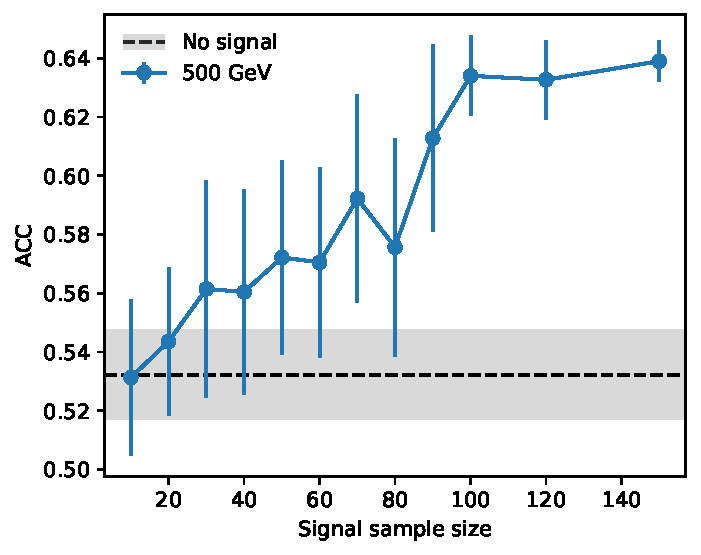
\includegraphics[width=0.55\textwidth]{ACC_vs_signal_sample_size-500GeV.pdf}
            \caption{The accuracy of CWoLa DNN training as a function of the signal size. The unit of sample size is the size of the ``1 times'' case. The error bar is the standard deviation of 10 training. The grey band is the error bar of the ``without signal'' case.}
            \label{fig:cwola_hunting_DNN_results_wo_pt_m_various_signal_size_500GeV}
        \end{figure}

        Figure~\ref{fig:cwola_hunting_DNN_results_wo_pt_m_various_signal_size_500GeV} is the training performance against the signal sample size. In this region, the performance increases when the signal size is increased. 120 times and 150 times samples are also generated and used in training. The accuracy is saturated at around 63\%.

        Similarly, for the $\text{1000 GeV}$ case, the DNN is trained on samples with sizes ranging from 1 to 10 times. Figure~\ref{fig:cwola_hunting_DNN_results_wo_pt_m_various_signal_size_1000GeV} is the training performance against the signal sample size. The performance is similar for all cases. The training accuracy is saturated at around 62\%.
        \begin{figure}[htpb]
            \centering
            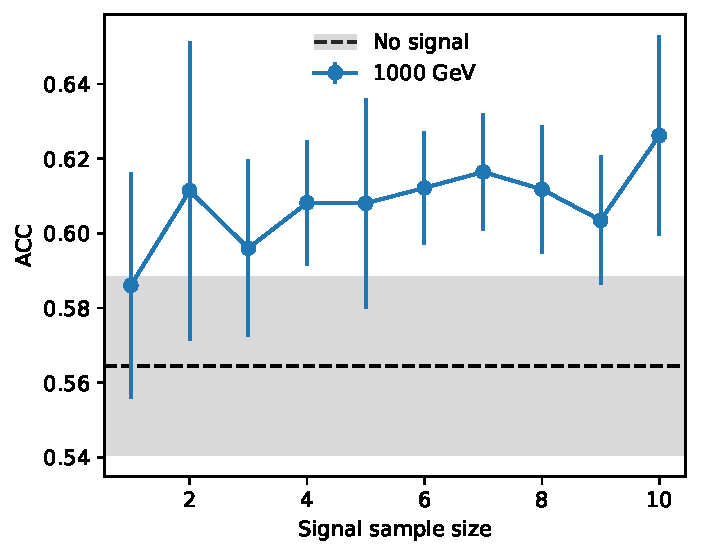
\includegraphics[width=0.55\textwidth]{ACC_vs_signal_sample_size-1000GeV.pdf}
            \caption{The performance of CWoLa DNN training as a function of the signal size. The unit of sample size is the size of the ``1 times'' case. The error bar is the standard deviation of 10 times training. The grey band is the error bar of the ``without signal'' case.}
            \label{fig:cwola_hunting_DNN_results_wo_pt_m_various_signal_size_1000GeV}
        \end{figure}

    % subsection enlarge_the_signal_sample_size (end)
    \subsection{Training with deeper model}% (fold)
    \label{sub:training_with_deeper_model}
        In Figure~\ref{fig:cwola_hunting_DNN_results_wo_pt_m_various_signal_size_1000GeV}, the performance of CWoLa DNN is quickly saturated. To investigate the impact of the model structure, the deeper DNN model is trained. In Section~\ref{sub:enlarge_the_signal_sample_size}, DNN consists of 2 hidden layers, while in this section we train the DNN with 4 hidden layers.

        The DNN is trained on signal sample size ranging from 1 to 500 times. Table~\ref{tab:cwola_hunting_DNN_results_wo_pt_m_enlarge_signal_size_deeper_model} and Figure~\ref{fig:cwola_hunting_DNN_results_wo_pt_m_various_signal_size_deeper_model_1000GeV} are the training results. The performance is generally better than the previous results (Table~\ref{tab:cwola_hunting_DNN_results_wo_pt_m_enlarge_signal_size}), even for the without signal case. It seems that the previous model structure is too simple and it limits the training performance. For the signal size within 1 time to 300 times, the performance increases when the signal size increases. After this region, the accuracy does not significantly improve. The accuracy is saturated at around 67\%, but this value is still better than the previous ones.

        \begin{table}[htpb]
            \centering
            \caption{The CWoLa DNN training results. The transverse momentum and invariant mass of Higgs candidates are removed from samples. 1 time and 0 times are the with signal and no signal case in Table~\ref{tab:cwola_hunting_DNN_results_wo_pt_m}. ACC is the best accuracy and AUC is the area under the ROC curve. The average and standard deviation of 10 training are presented.}
            \label{tab:cwola_hunting_DNN_results_wo_pt_m_enlarge_signal_size_deeper_model}
            \begin{tabular}{c|c|cc}
                $m_H$ (GeV)           & times & ACC               & AUC               \\ \hline
                \multirow{4}{*}{1000} & 1     & $0.613 \pm 0.017$ & $0.649 \pm 0.021$ \\
                                      & 10    & $0.622 \pm 0.018$ & $0.673 \pm 0.033$ \\
                                      & 100   & $0.639 \pm 0.022$ & $0.695 \pm 0.034$ \\
                                      & 0     & $0.602 \pm 0.022$ & $0.643 \pm 0.042$
            \end{tabular}
        \end{table}
        \begin{figure}[htpb]
            \centering
            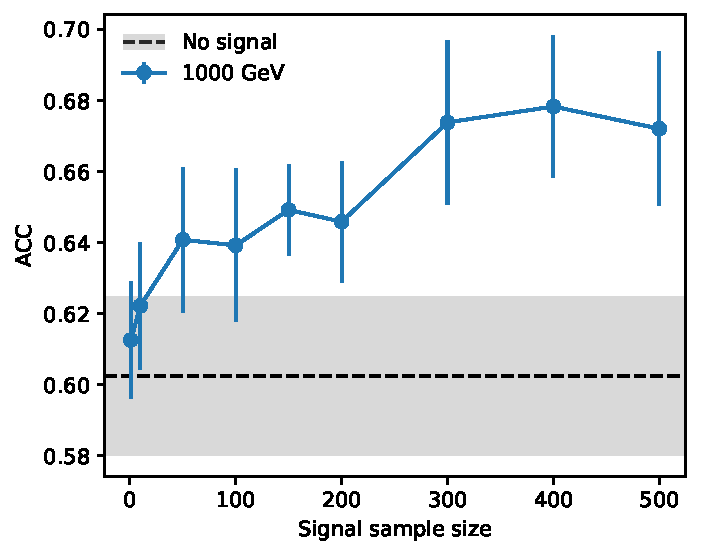
\includegraphics[width=0.55\textwidth]{ACC_vs_signal_sample_size_deeper_model-1000GeV.pdf}
            \caption{The performance of CWoLa DNN training as a function of the signal size. The unit of sample size is the size of the ``1 times'' case. The error bar is the standard deviation of 10 times training. The grey band is the error bar of the ``without signal'' case.}
            \label{fig:cwola_hunting_DNN_results_wo_pt_m_various_signal_size_deeper_model_1000GeV}
        \end{figure}
    % subsection training_with_deeper_model (end)
% section cwola_hunting (end)
\section{Physical data augmentation}% (fold)
\label{sec:physical_data_augmentation}
    The physical augmentations are inspired by Reference~\cite{Dillon:2023zac}, which considers the rotation and smearing augmentations. These augmentations reflect both the symmetries in the physical event and the experimental resolution of the detector.
    \subsection{Original training data}% (fold)
    \label{sub:original_training_data}
        The signal is the resonant Higgs boson pairs production in the four-$b$ quarks channel. This section produces the Higgs boson pair by the heavy CP-even scalar $H$ with mass $m_H = \text{500 GeV}$. The background consists of QCD multi-jet events. The basic requirement is the ``four-tag cut,'' which requires at least four $b$-tagged $R = 0.4$ anti-$k_t$ jets with $p_\text{T} > \text{40 GeV}$ and $\abs{\eta} < 2.5$. Only the events passing the four-tag cut are used in the following analysis.

        The training samples consist of 50k signal events and 50k background events and the testing samples consist of 5k signal events and 5k background events.

        The Higgs candidates are reconstructed by the $\text{min-}\Delta R$ pairing method. The input features are similar to the previous case (Table~\ref{tab:DNN_variables}), but the $b$-tagging information is excluded.
    % subsection original_training_data (end)
    \subsection{Physical augmentation}% (fold)
    \label{sub:physical_augmentation}
        We consider three different physical augmentations.

        \begin{enumerate}
            \item Azimuthal rotation: The final state is rotated by an angle $\phi$ randomly sampled from $[0, 2\pi]$.
            \item $\eta-\phi$ smearing: The $\left( \eta,\phi \right) $ coordinate of Higgs candidates are resampled according to a Normal distribution centered on the original coordinate and with a standard deviation inversely proportional to the $p_{\text{T}}$
                \begin{equation}
                    \eta' \sim \mathcal{N}\left(\eta, \frac{\Lambda}{p_{\text{T}}}\right), \quad \phi' \sim \mathcal{N}\left(\phi, \frac{\Lambda}{p_{\text{T}}}\right)
                \end{equation}
                where $\eta', \phi'$ are the augmented coordinate, $p_{\text{T}}$ is the transverse momentum of the Higgs candidate, and the smearing scale is set to be $\Lambda = \text{10 GeV}$.
            \item $p_\text{T}$ smearing: The $p_{\text{T}}$ of Higgs candidates are resampled according to
                \begin{equation}
                    p_{\text{T}}' \sim \mathcal{N}\left( p_{\text{T}}, f(p_{\text{T}}) \right), \quad f(p_{\text{T}}) = \sqrt{0.052 p_{\text{T}}^2 + 1.502p_{\text{T}}}
                \end{equation}
                where $p_{\text{T}}'$ is the augmented transverse momentum, $f\left( p_\text{T} \right) $ is the energy smearing applied by \verb|Delphes| (the $p_{\text{T}}$'s are normalised by $\text{1 GeV}$).
        \end{enumerate}

        Figure~\ref{fig:eta_phi_smearing_eta_distribution}, \ref{fig:eta_phi_smearing_phi_distribution} and \ref{fig:pt_smearing_pt_distribution} are the distributions before and after the augmentation. The distributions for the $\eta-\phi$ smearing are similar for both cases. For $p_\text{T}$ smearing, the peak broadens and the transverse momentum distribution looks smoother.
        \begin{figure}[htpb]
            \centering
            \subfloat[Leading Higgs]{
                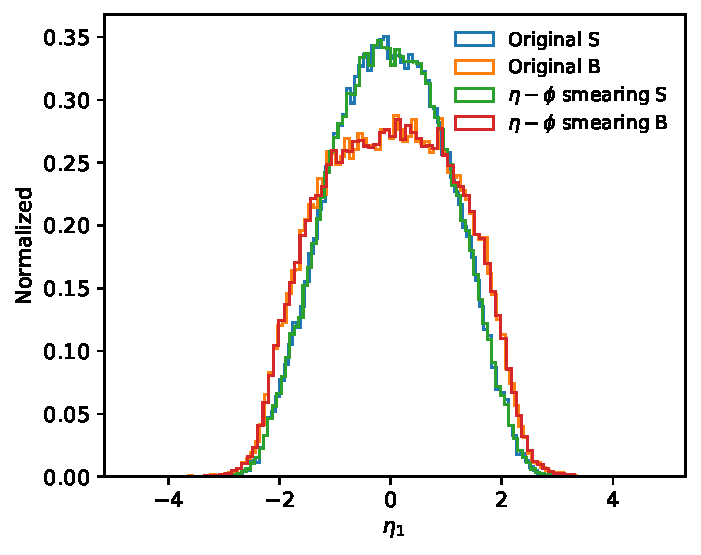
\includegraphics[width=0.45\textwidth]{eta1_distribution_eta_phi_smearing.pdf}
            }
            \subfloat[Sub-leading Higgs]{
                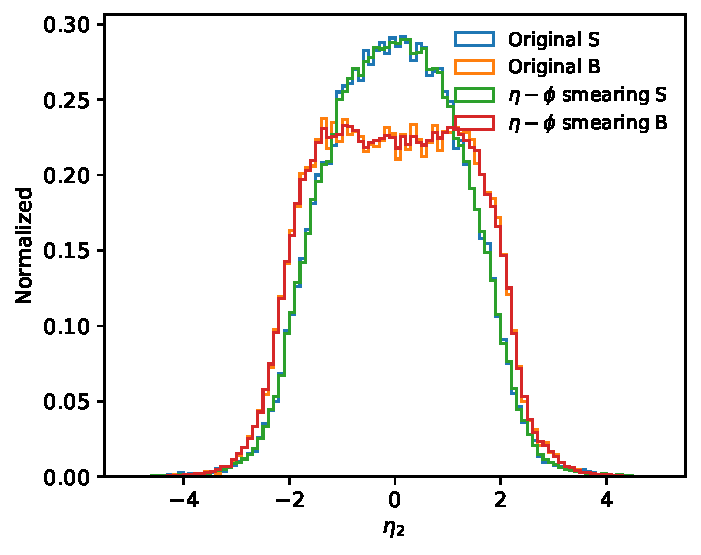
\includegraphics[width=0.45\textwidth]{eta2_distribution_eta_phi_smearing.pdf}
            }
            \caption{The pseudorapidity distribution before and after the $\eta-\phi$ smearing augmentation. $\eta_1$ and $\eta_2$ are the pseudorapidities of the leading and the sub-leading Higgs candidate, respectively.}
            \label{fig:eta_phi_smearing_eta_distribution}
        \end{figure}
        \begin{figure}[htpb]
            \centering
            \subfloat[Leading Higgs]{
                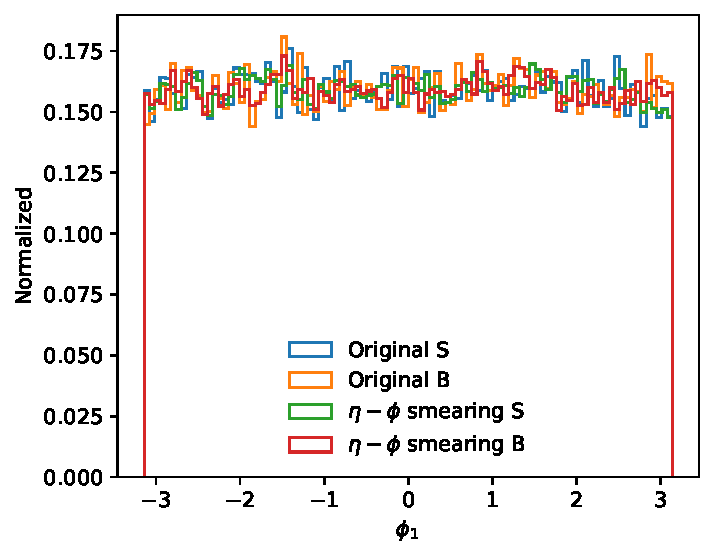
\includegraphics[width=0.45\textwidth]{phi1_distribution_eta_phi_smearing.pdf}
            }
            \subfloat[Sub-leading Higgs]{
                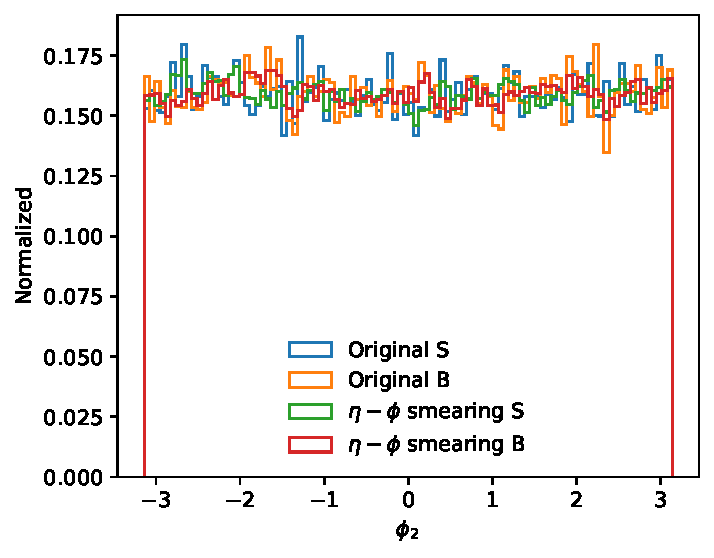
\includegraphics[width=0.45\textwidth]{phi2_distribution_eta_phi_smearing.pdf}
            }
            \caption{The azimuthal angle distribution before and after the $\eta-\phi$ smearing augmentation. $\phi_1$ and $\phi_2$ are the azimuthal angles of the leading and the sub-leading Higgs candidate, respectively.}
            \label{fig:eta_phi_smearing_phi_distribution}
        \end{figure}
        \begin{figure}[htpb]
            \centering
            \subfloat[Leading Higgs]{
                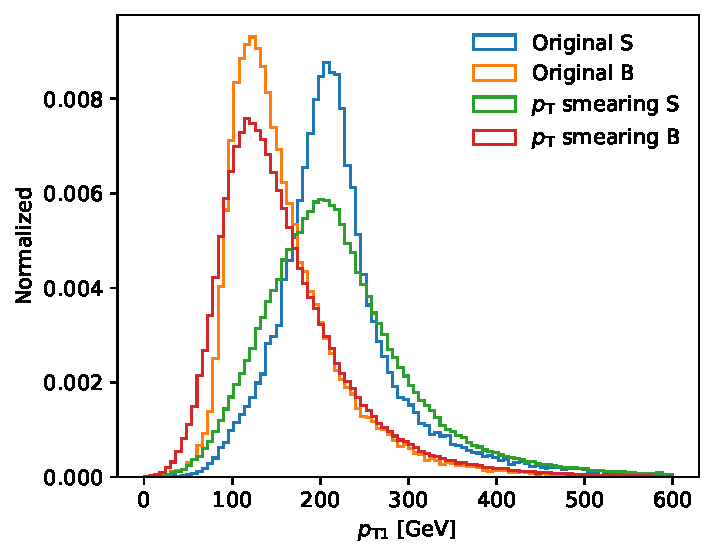
\includegraphics[width=0.45\textwidth]{pt1_distribution_pt_smearing.pdf}
            }
            \subfloat[Sub-leading Higgs]{
                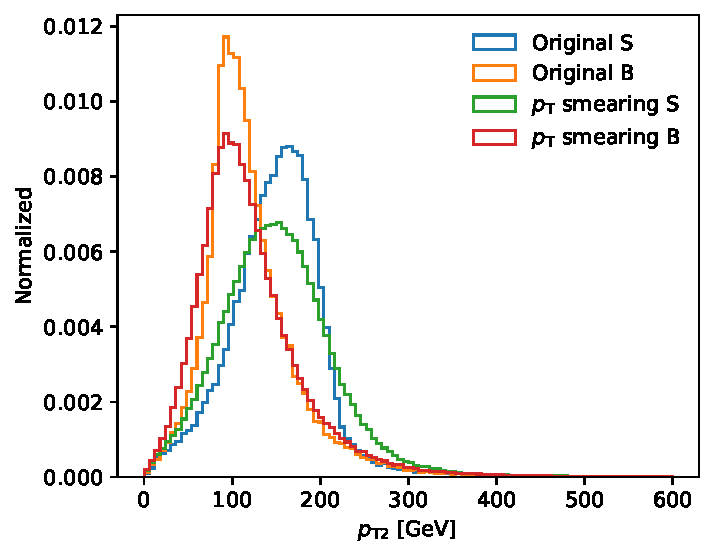
\includegraphics[width=0.45\textwidth]{pt2_distribution_pt_smearing.pdf}
            }
            \caption{The transverse momentum distribution before and after the $p_{\text{T}}$ smearing augmentation. $p_{\text{T1}}$ and $p_{\text{T2}}$ are the transverse momentum of the leading and the sub-leading Higgs candidates, respectively.}
            \label{fig:pt_smearing_pt_distribution}
        \end{figure}

        For each type of augmentation, we test ``$n$ times augmentation'' with different $n$. The $n$ times augmentation means for one original sample, we generate $n$ augmented samples. Additionally, we test another case that applies all augmentations at the same time.
    % subsection physical_augmentation (end)
    \subsection{Training results}% (fold)
    \label{sub:training_results_physical_augmentation}

        Table~\ref{tab:original_sample_training_results} presents the DNN classification training results of the original sample. Table~\ref{tab:augmentation_sample_training_results} are the training results of the augmented samples. For each type of augmentation, they all can improve the ACC by about 4\%. The differences among the various augmentation are not significant. The 10-times augmentation has the best results, but the difference between the 5-times and 10-times augmentation is tiny. It seems that the performance of this classifier is saturated.
        \begin{table}[htpb]
            \centering
            \caption{The training results of original samples. ACC is the best accuracy and AUC is the area under the ROC curve. The average and standard deviation of 10 training are presented.}
            \label{tab:original_sample_training_results}
            \begin{tabular}{c|c}
                & Original \\ \hline
            ACC & $0.845 \pm 0.015$    \\
            AUC & $0.917 \pm 0.005$
            \end{tabular}
        \end{table}
        \begin{table}[htpb]
            \centering
            \caption{The training results of augmented samples. ``+ 3 times'' means the training sample consists of the original sample and 3 times the augmented sample. ACC is the best accuracy and AUC is the area under the ROC curve. The average and standard deviation of 10 training are presented.}
            \label{tab:augmentation_sample_training_results}
            \begin{tabular}{c|c|cccc}
                Sample                      &     & Rotation          & $\eta-\phi$ smear & $p_{\text{T}}$ smear & All               \\ \hline
                \multirow{2}{*}{+ 3 times}  & ACC & $0.880 \pm 0.007$ & $0.879 \pm 0.010$ & $0.882 \pm 0.003$    & $0.875 \pm 0.011$ \\
                                            & AUC & $0.950 \pm 0.007$ & $0.949 \pm 0.008$ & $0.951 \pm 0.003$    & $0.942 \pm 0.012$ \\ \hline
                \multirow{2}{*}{+ 5 times}  & ACC & $0.887 \pm 0.002$ & $0.887 \pm 0.001$ & $0.890 \pm 0.002$    & $0.889 \pm 0.003$ \\
                                            & AUC & $0.955 \pm 0.001$ & $0.955 \pm 0.001$ & $0.957 \pm 0.001$    & $0.956 \pm 0.001$ \\ \hline
                \multirow{2}{*}{+ 10 times} & ACC & $0.889 \pm 0.001$ & $0.889 \pm 0.002$ & $0.892 \pm 0.002$    & $0.892 \pm 0.002$ \\
                                            & AUC & $0.956 \pm 0.001$ & $0.956 \pm 0.001$ & $0.958 \pm 0.001$    & $0.958 \pm 0.000$
            \end{tabular}
        \end{table}


    % subsection training_results_physical_augmentation (end)

    \subsection{Deeper model}% (fold)
    \label{sub:deeper_model}
        In Section~\ref{sub:training_results_physical_augmentation}, the DNN model consists of 2 hidden layers, each containing 64 hidden nodes. To explore the impact of the model structure, the deeper DNN model is trained. We investigate the performance of the DNN model with 5 hidden layers.

        \begin{table}[htpb]
            \centering
            \caption{The training results of deeper DNN model. ``+ 3 times'' means the training sample consists of the original sample and 3 times the augmented sample. ACC is the best accuracy and AUC is the area under the ROC curve. The average and standard deviation of 10 training are presented.}
            \label{tab:augmentation_training_results_deeper_model}
            \begin{tabular}{l|c|cccc}
            Sample                            &     & Original          & + 3 times         & + 5 times         & + 10 times        \\ \hline
            \multirow{2}{*}{All augmentation} & ACC & $0.864 \pm 0.005$ & $0.890 \pm 0.002$ & $0.890 \pm 0.002$ & $0.884 \pm 0.005$ \\
                                              & AUC & $0.928 \pm 0.005$ & $0.957 \pm 0.001$ & $0.957 \pm 0.001$ & $0.949 \pm 0.005$
            \end{tabular}
        \end{table}

        Table~\ref{tab:augmentation_training_results_deeper_model} are the training results with a deeper DNN model. Models are only trained on the ``All augmentation'' sample because from Table~\ref{tab:augmentation_sample_training_results} we found that four augmentation methods yielded similar results. The results show that the augmented sample can improve ACC to 89\%, even from the ``+ 3 times'' case and this accuracy value is similar to the previous test. These findings suggest that the classifier may have reached a saturation point and point out the difficulty of further improving accuracy on this test sample.
    % subsection deeper_model (end)
% section physical_data_augmentation (end)
\section{Hidden Valley model}% (fold)
\label{sec:hidden_valley_model}
    \subsection{Sample generation}% (fold)
    \label{sub:sample_generation}
        The signal process is $f \overline{f} \to Z_V$, where $Z_V$ is the massive gauge boson linking SM and the dark sector. The hidden $Z_V$ boson would decay to a pair of dark quark $q_V \overline{q}_V$, leading to two jets in the detector. The signal sample is generated by \verb|Pythia| and the detector simulation is done by \verb|Delphes|. The $\text{anti-}k_t$ algorithm is utilized for jet reconstruction with parameter $R = 0.8$. Some parameters are listed in Table~\ref{tab:hv_model_signal_parameter}.

        \begin{table}[htpb]
            \centering
            \caption{The parameter setting for the Hidden Valley model. ``490010x:m0 = 10.3306; x=1,2,3'' means x should be replaced by 1,2,3 in Pythia card.}
            \label{tab:hv_model_signal_parameter}
            \begin{tabular}{c|c|l}
                Parameter                  & Value       & Pythia card                             \\ \hline
                $M_{Z_V}$                  & 5.5 TeV     & 4900023:m0 = 5500                       \\
                $\sqrt{s}$                 & 13 TeV      &                                         \\
                $\Lambda_{\text{D}}$       & 10 GeV      & HiddenValley:Lambda = 10.0              \\
                $m_{\pi_{\text{D}}}$       & 10 GeV      & 4900x1:m0 = 10.0; x=11,21,31,22,32,33   \\
                $m_{\rho_{\text{D}}}$      & 26.944 GeV  & 4900x3:m0 = 26.944; x=11,21,31,22,32,33 \\
                $m_{q,\text{constituent}}$ & 10.3306 GeV & 490010x:m0 = 10.3306; x=1,2,3
            \end{tabular}
        \end{table}

        The background sample is the SM QCD di-jet. This process is generated at $\sqrt{s} = \text{13 TeV}$. Following are the \verb|MadGraph| scripts for generating background samples:
        \begin{verbatim}
            generate p p > j j
            output ppjj
            launch ppjj

            shower=Pythia8
            detector=Delphes
            analysis=OFF
            madspin=OFF
            done

            Cards/delphes_card_CMS.dat

            set run_card nevents 10000
            set run_card ebeam1 6500.0
            set run_card ebeam2 6500.0

            set run_card ptj 700
            set run_card etaj 2.2
            set run_card mmjj 3000

            done
        \end{verbatim}
    % subsection sample_generation (end)
    \subsection{Problem for generating signal sample}% (fold)
    \label{sub:problem_for_generating_signal_sample}
        Error messages:
        \begin{verbatim}
            PYTHIA Error: input string not found in settings databases::
              HiddenValley:separateFlav    = on! Consider different flavours

            PYTHIA Error: input particle not found in Particle Data Table:
              4900102:m0                   = 10.3306

            ...
        \end{verbatim}

        Solution: This problem arises from the \verb|Pythia| version. At first, \verb|Pythia 8.306| is used to generate signal samples. Some features are not included in this version. We should use \verb|Pythia 8.307| at least. More details between 8.306 and 8.307 can be found in this \href{https://pythia.org/history/}{page}.
    % subsection problem_for_generating_signal_sample (end)
    \subsection{Sample selection}% (fold)
    \label{sub:sample_selection}
        The selection cuts after the \verb|Delphes| simulation:
        \begin{itemize}
            \item $n_j$ cut: The number of jets should be greater than or equal to 2.
            \item $p_{\text{T}}$ cut: The transverse momentum of two highest $p_{\text{T}}$ jets should greater $\text{750 GeV}$.
            \item $\eta$ cut: The $\eta$ range of two highest  $p_{\text{T}}$ jets are require $\abs{\eta} < 2$.
            \item Signal region: Total invariant mass of two leading jets $m_{jj}$ belonging to $[4700,5500]$.
            \item Sideband region: Total invariant mass of two leading jets $m_{jj}$ belonging to $[4300,4700] \cup [5500,5900]$.
        \end{itemize}

        Table~\ref{tab:HVmodel_cutflow_number} is the cutflow number at different selection cuts. Figure~\ref{fig:HVmodel_pt_distribution} is transverse momentum distribution after $n_j$ cut. Figure~\ref{fig:HVmodel_mjj_distribution} is the $m_{jj}$ distribution after the $\eta$ cut.
        \begin{table}[htpb]
            \centering
            \caption{The number of passing events and passing rates for signal and background processes at different selection cuts.}
            \label{tab:HVmodel_cutflow_number}
            \begin{tabular}{l|rr|rr}
            Cut                & Signal & pass rate & Background & pass rate \\ \hline
            Total              & 100000  & 1         & 100000     & 1         \\
            $n_j$ cut          & 99996   & 1.00      & 99963      & 1.00      \\
            $p_{\text{T}}$ cut & 90901   & 0.91      & 57832      & 0.58      \\
            $\eta$ cut         & 89800   & 0.90      & 55523      & 0.56      \\ \hline
            SR region          & 55844   & 0.56      & 1991       & 0.02      \\
            SB region          & 16079   & 0.16      & 3090       & 0.03
            \end{tabular}
        \end{table}

        \begin{figure}[htpb]
            \centering
            \subfloat[Signal]{
                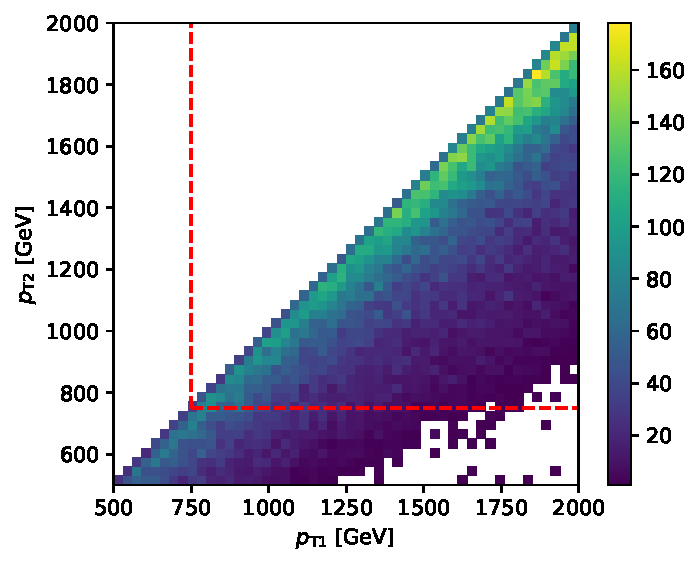
\includegraphics[width=0.45\textwidth]{HVmodel_pt_distribution-sig.pdf}
            }
            \subfloat[Background]{
                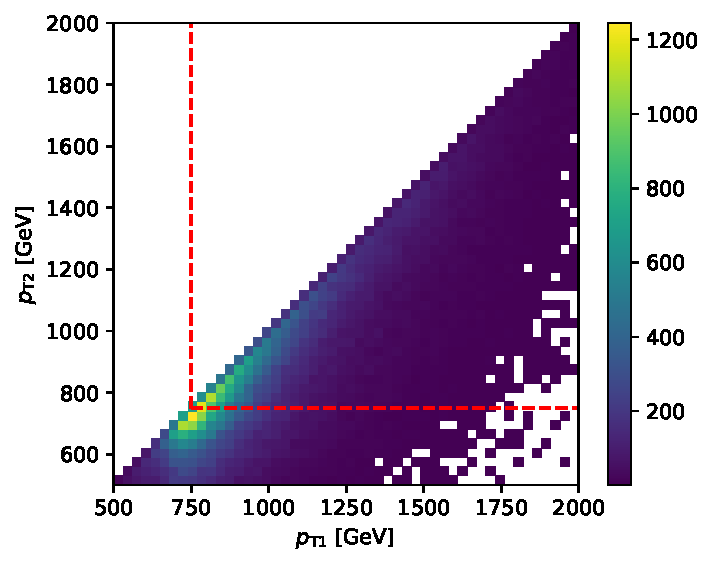
\includegraphics[width=0.45\textwidth]{HVmodel_pt_distribution-bkg.pdf}
            }
            \caption{The transverse momentum distribution of leading and sub-leading jets. The red dashed lines are the $p_{\text{T}}$ cut.}
            \label{fig:HVmodel_pt_distribution}
        \end{figure}

        \begin{figure}[htpb]
            \centering

            \subfloat[My plot]{
                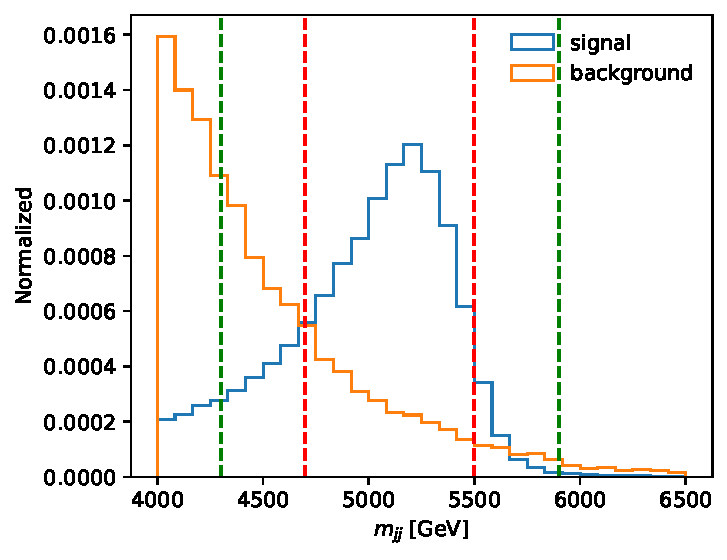
\includegraphics[width=0.45\textwidth]{HVmodel_mjj_distribution.pdf}
            }
            \subfloat[Zong-En's plot]{
                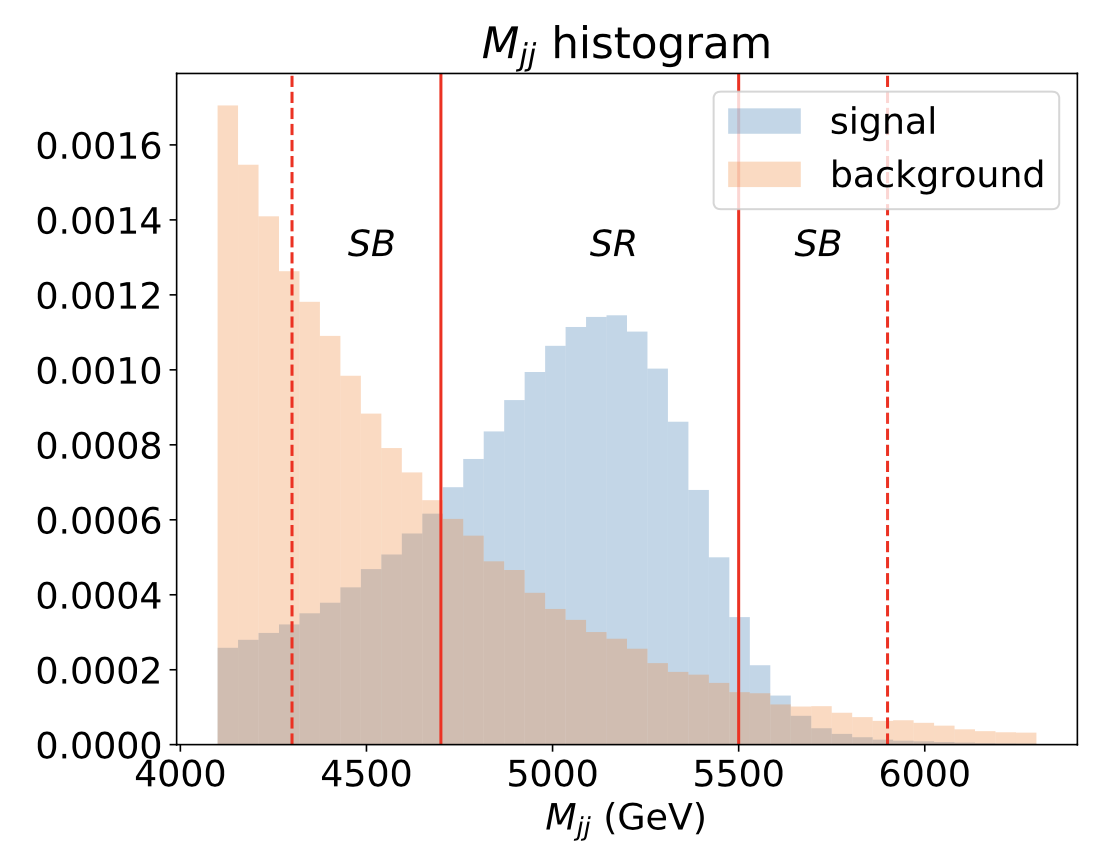
\includegraphics[width=0.50\textwidth]{HVmodel_mjj_distribution-Zong-En.png}
            }
            \caption{The total invriant mass $m_{jj}$ distribution of signal and background samples. In my plot, the signal region is between the red dashed lines. The sideband region is between the green dashed lines and excludes the signal region.}
            \label{fig:HVmodel_mjj_distribution}
        \end{figure}
    % subsection sample_selection (end)
    \subsection{Jet image}% (fold)
    \label{sub:jet_image}
        We can construct the jet image from the event passing the selection cuts described in Section~\ref{sub:sample_selection}. The jet image is constructed for each jet separately so that we would obtain two for each event. They are treated as two channels of a picture. The following steps construct the jet image:
        \begin{enumerate}
            \item Centralization: Compute the $p_{\text{T}}$ weighted center in $\left( \eta,\phi \right) $ coordinates, then shift this point to origin.
            \item Rotation: Rotate the highest intensity axis to the $\eta$ axis.
            \item Flipping: Flip the highest intensity quadrant to the first quadrant.
            \item Pixelating in $\eta \in [-1,1],\ \phi \in [-1,1]$ box, with $75\times 75$ pixels.
        \end{enumerate}

        Figure~\ref{fig:HVmodel_jet_image_one_event} is the jet images of a single event. Figure~\ref{fig:HVmodel_jet_image_average} is the average jet image.

        \begin{figure}[htpb]
            \centering
            \subfloat[Signal]{
                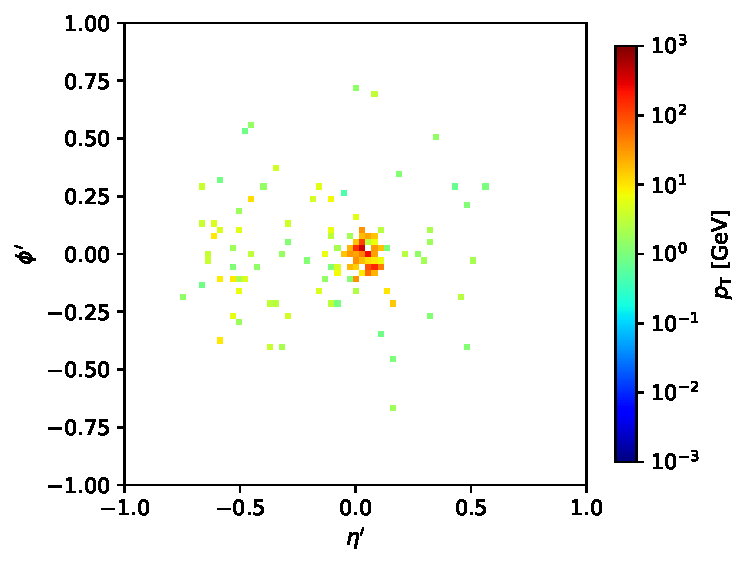
\includegraphics[width=0.45\textwidth]{HVmodel_signal_jet_image_one_event.pdf}
            }
            \subfloat[Background]{
                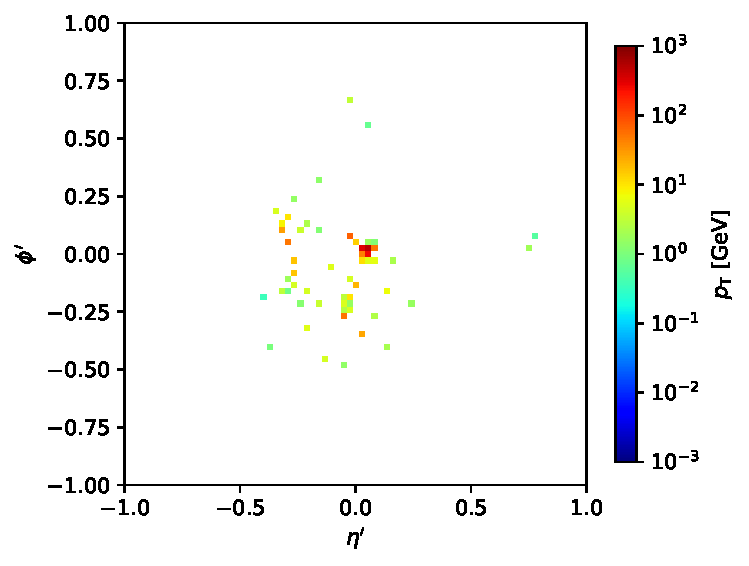
\includegraphics[width=0.45\textwidth]{HVmodel_background_jet_image_one_event.pdf}
            }
            \caption{The jet images of the leading jet in the signal region. The $\eta'$ and $\phi'$ are the coordinates after the preprocessing (centralization, rotation, flipping).}
            \label{fig:HVmodel_jet_image_one_event}
        \end{figure}
        \begin{figure}[htpb]
            \centering
            \subfloat[Signal]{
                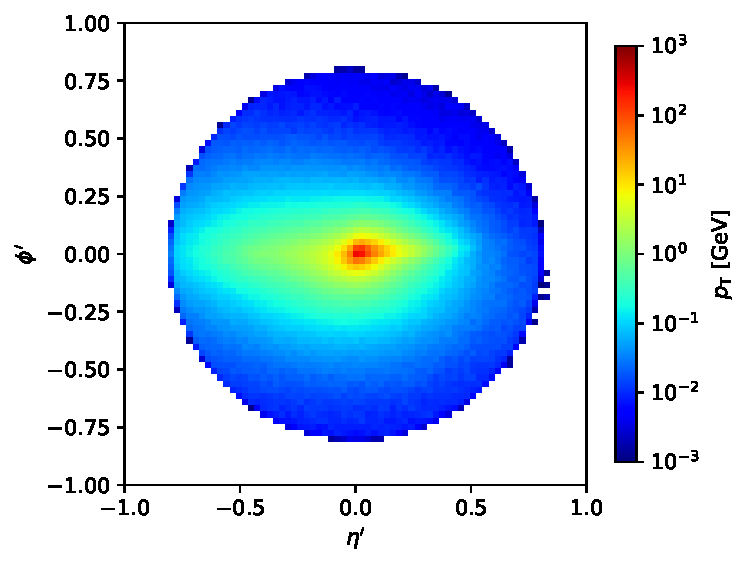
\includegraphics[width=0.45\textwidth]{HVmodel_signal_jet_image_average.pdf}
            }
            \subfloat[Background]{
                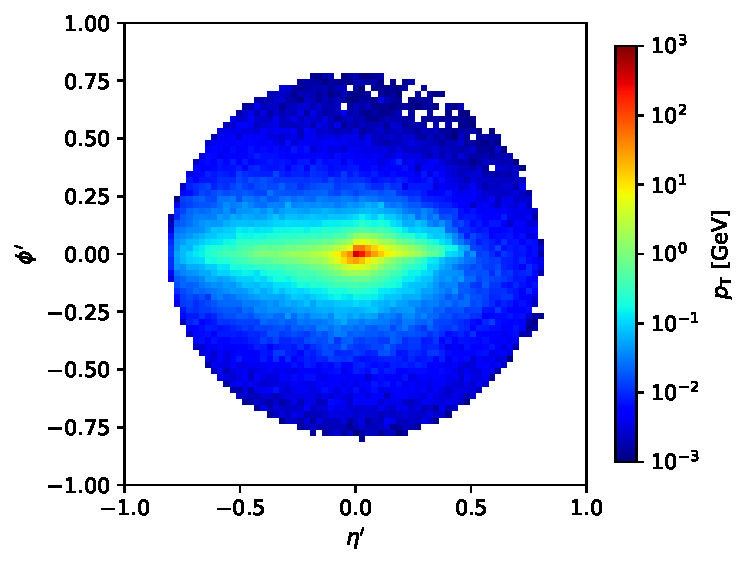
\includegraphics[width=0.45\textwidth]{HVmodel_background_jet_image_average.pdf}
            }
            \caption{The average jet images of the leading jet in the signal region. The $\eta'$ and $\phi'$ are the coordinates after the preprocessing (centralization, rotation, flipping). The number of the signal events is 56k. The number of the background events is 20k.}
            \label{fig:HVmodel_jet_image_average}
        \end{figure}
    % subsection jet_image (end)
    \subsection{Datasets}% (fold)
    \label{sub:datasets}
        The total cross-section of the background events is $6837 \text{ fb}$. From Table~\ref{tab:HVmodel_cutflow_number}, we can compute the corresponding cross-sections of signal and sideband regions are $136.1 \text{ fb}$ and $211.2 \text{ fb}$, respectively. Thus, the numbers of events in signal and sideband region are 19k and 29k at luminosity $\mathcal{L} = 139 \text{ fb}^{-1}$.

        The training sample sizes are summarized in Table~\ref{tab:training_sample_size_cwola_hunting_hv}.
        \begin{table}[htpb]
            \centering
            \caption{The training sample size for the mixed sample. We set sensitivity $S / \sqrt{B} = 1$ in the signal region and evaluate the number of events in the signal region. Then, the number of events in the sideband region can be obtained from Table~\ref{tab:HVmodel_cutflow_number}.}
            \label{tab:training_sample_size_cwola_hunting_hv}
            \begin{tabular}{c|cc}
                                & \multicolumn{2}{c}{True label} \\
                Mixed sample    & Signal       & Background      \\ \hline
                Signal region   & 138          & 19k             \\
                Sideband region & 40           & 29k
            \end{tabular}
        \end{table}

        The pure testing sample consists of 10k signal events and 10k background events selected from the signal region.
    % subsection datasets (end)
    \subsection{Training CNN}% (fold)
    \label{sub:training_cnn}
        The CNN model structure is summarized in Figure~\ref{fig:cnn_model_structure}. The internal node uses the rectified leaner unit (ReLU) as the activation function. The loss function is Categorical cross-entropy, and we use the Adam optimizer to optimize the loss function.
        \begin{figure}[htpb]
            \centering
            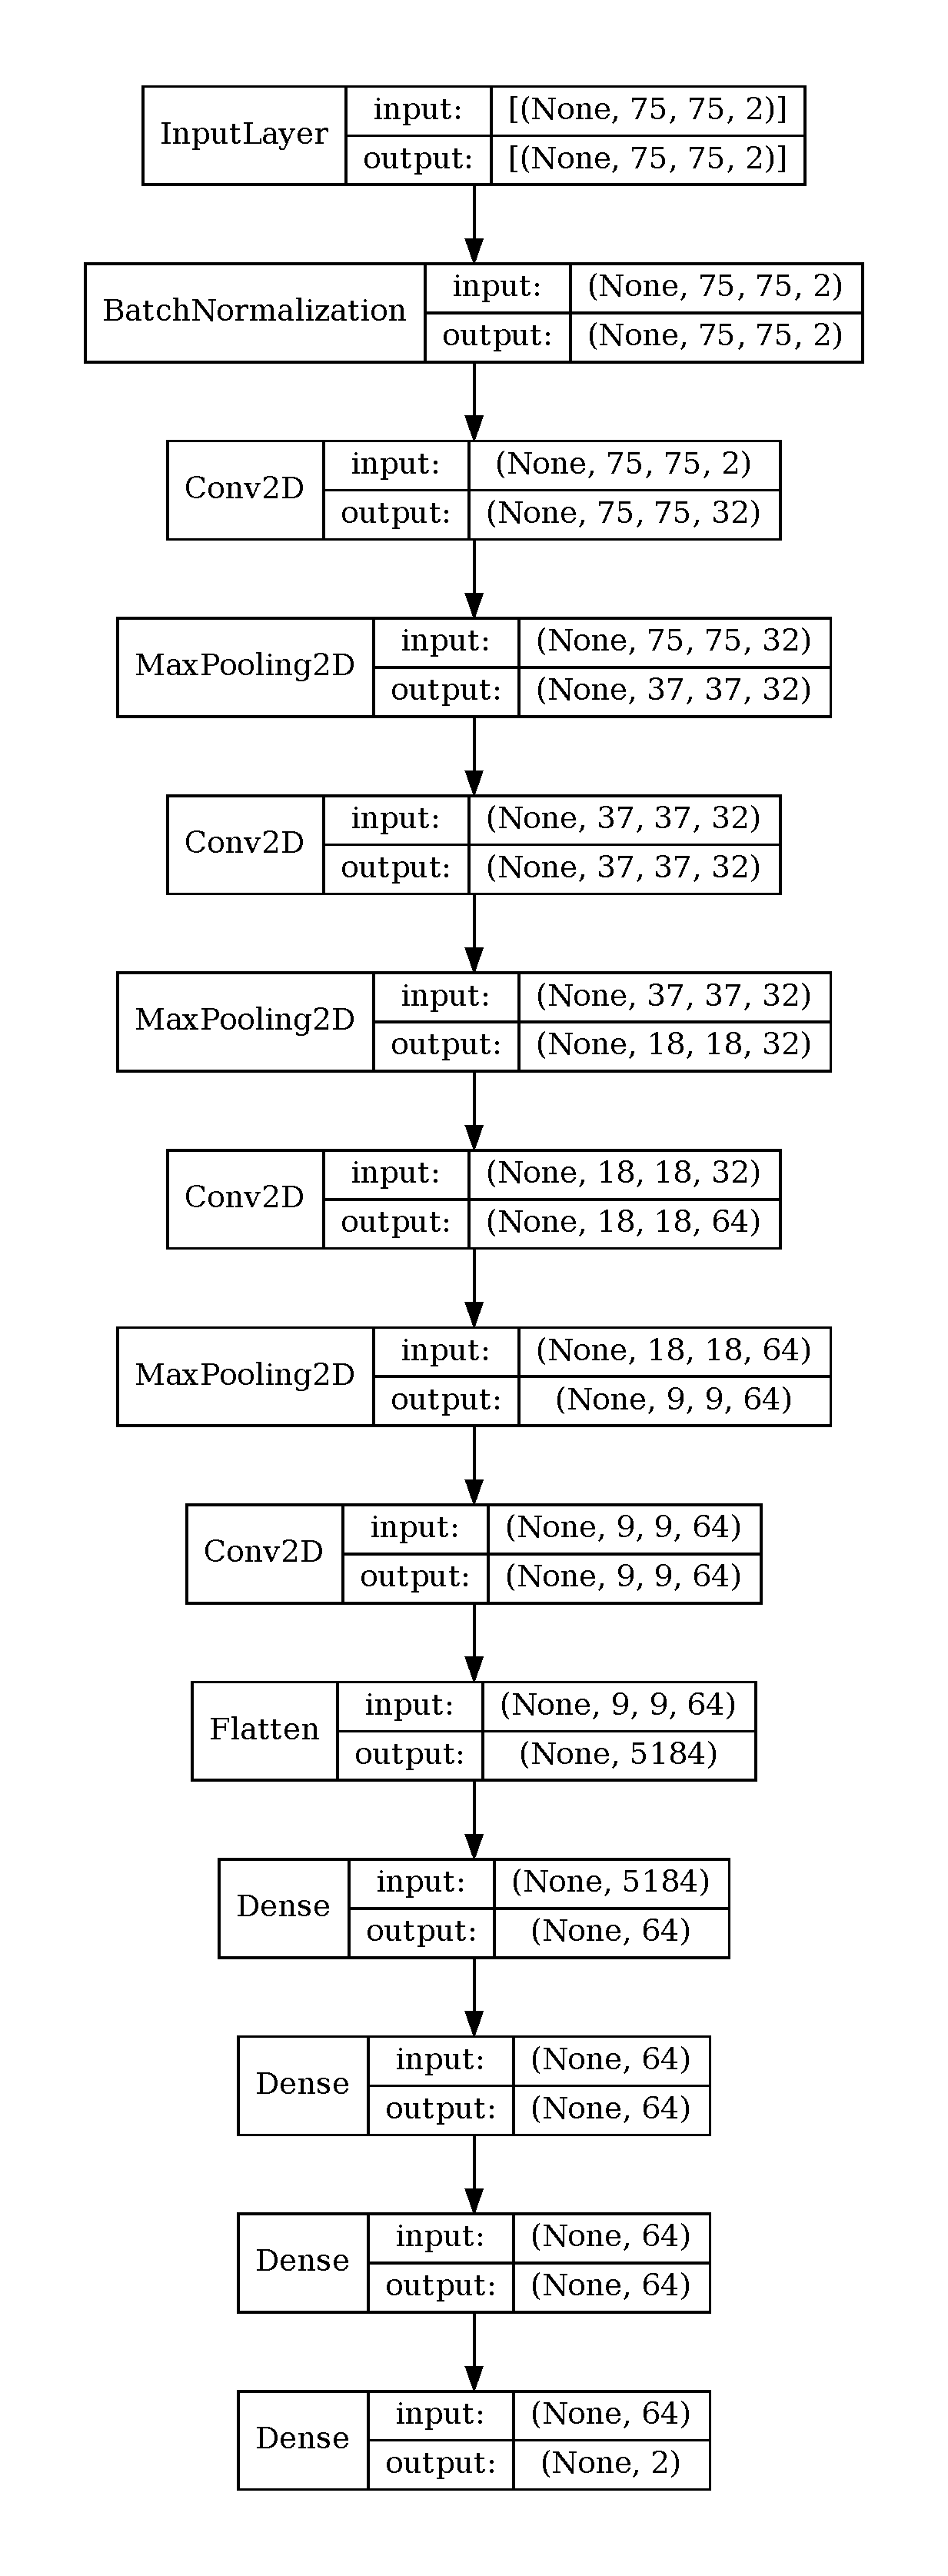
\includegraphics[width=0.45\textwidth]{CNN_model_structure.pdf}
            \caption{For first and second Conv2D layers, the kernel sizes are $5 \times 5$. For third and fourth Conv2D layers, the kernel sizes are $3 \times 3$.}
            \label{fig:cnn_model_structure}
        \end{figure}
    % subsection training_cnn (end)
    \subsection{Hidden Valley model training results}% (fold)
    \label{sub:hidden_valley_model_training_results}
        The CNN is trained on samples with sensitivity $S / \sqrt{B}$ ranging from 1 to 10. Figure~\ref{fig:cwola_hunting_cnn_acc} presents the training results. These numbers are evaluated from the pure samples. The CNN cannot learn useful information for the case with a sensitivity $S / \sqrt{B} \le  5$, so the ACC is 0.5. After this region, the accuracy demonstrates a significant improvement. It seems that the CNN model surpasses a certain threshold.

        \begin{figure}[htpb]
            \centering
            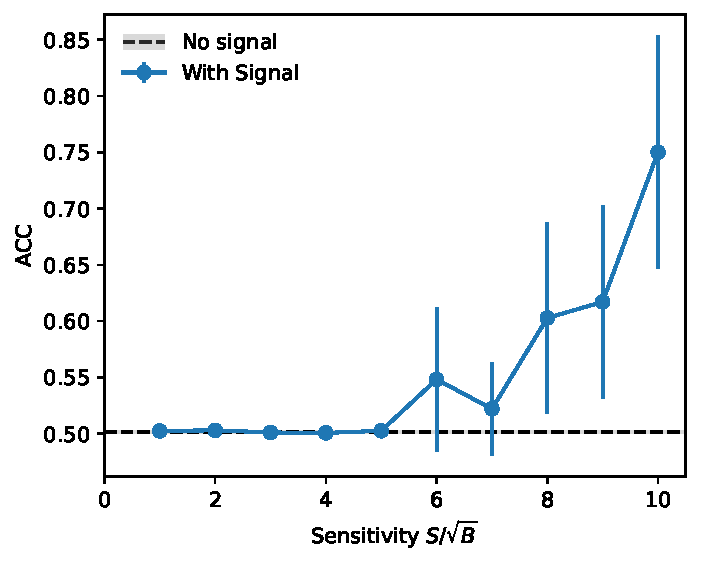
\includegraphics[width=0.55\textwidth]{HVmodel_CWoLa_CNN.pdf}
            \caption{The performance of CWoLa CNN training as a function of the sensitivity. The error bar is the standard deviation of 10 times training. The grey band is the error bar of the ``without signal'' case. For sensitivity less than 5, the error bar is too small to see.}
            \label{fig:cwola_hunting_cnn_acc}
        \end{figure}
    % subsection hidden_valley_model_training_results (end)
    \subsection{Data process procedure}% (fold)
    \label{sub:data_process_procedure}
        \begin{enumerate}
            \item Generate the sample file in \verb|.root| format. Following Section~\ref{sub:sample_generation}.
            \item Apply the selection cuts described in Section~\ref{sub:sample_selection} and save the event passing the cuts in \verb|HDF5| format. The file contains the information listed below
                \begin{itemize}
                    \item The $\left( p_{\text{T}}, \eta, \phi \right) $ of leading and sub-leading jet constituents.
                    \item Total invariant mass $m_{jj}$.
                    \item Type of event: 1 for signal, 0 for background.
                \end{itemize}
            \item Make mixed sample in \verb|HDF5| format. Following Section~\ref{sub:datasets}, we can compute the size of datasets.
            \item Apply data augmentation in \verb|HDF5| format. Following Section~\ref{sub:data_augmentation}.
            \item Generate the jet image from \verb|HDF5| data.
        \end{enumerate}
        Note the preprocessing is done in step 5. If we do the preprocessing many times, the rounding errors would break the jet image.
    % subsection data_process_procedure (end)
    \subsection{Data augmentation}% (fold)
    \label{sub:data_augmentation}
        To reduce the threshold, the data augmentation technique is tested. Similar to the Section~\ref{sub:physical_augmentation}, we apply the $\eta-\phi$ smearing on our training sample. Specifically, the $\left( \eta,\phi \right) $ coordinate of jet constituents are resampled according to a Normal distribution centered on the original coordinate and with a standard deviation inversely proportional to the $p_{\text{T}}$
        \begin{equation}
            \eta' \sim \mathcal{N}\left(\eta, \frac{\Lambda}{p_{\text{T}}}\right), \quad \phi' \sim \mathcal{N}\left(\phi, \frac{\Lambda}{p_{\text{T}}}\right)
        \end{equation}
        where $\eta', \phi'$ are the augmented coordinate, $p_{\text{T}}$ is the transverse momentum of the jet constituent, and the smearing scale is set to be $\Lambda = \text{100 MeV}$.

        Figure~\ref{fig:eta_phi_smearing_jet_constituent_jet_image} and \ref{fig:eta_phi_smearing_phi_jet_constituent_average_jet_image} are the jet image before and after the augmentation. The jet images look similar before and after the augmentation, but not the same.
        \begin{figure}[htpb]
            \centering
            \subfloat[Before augmentation]{
                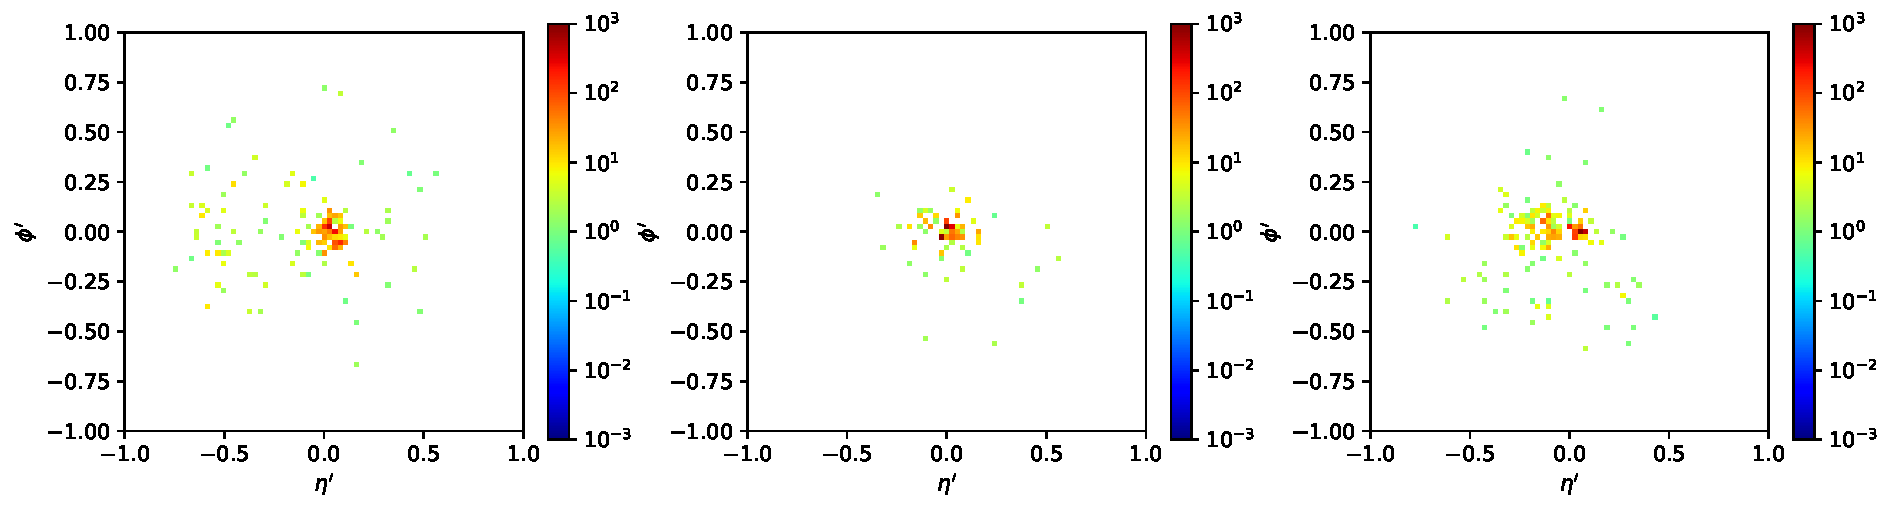
\includegraphics[width=0.95\textwidth]{HVmodel_jet_image_one_event_original.pdf}
            } \\
            \subfloat[After augmentation]{
                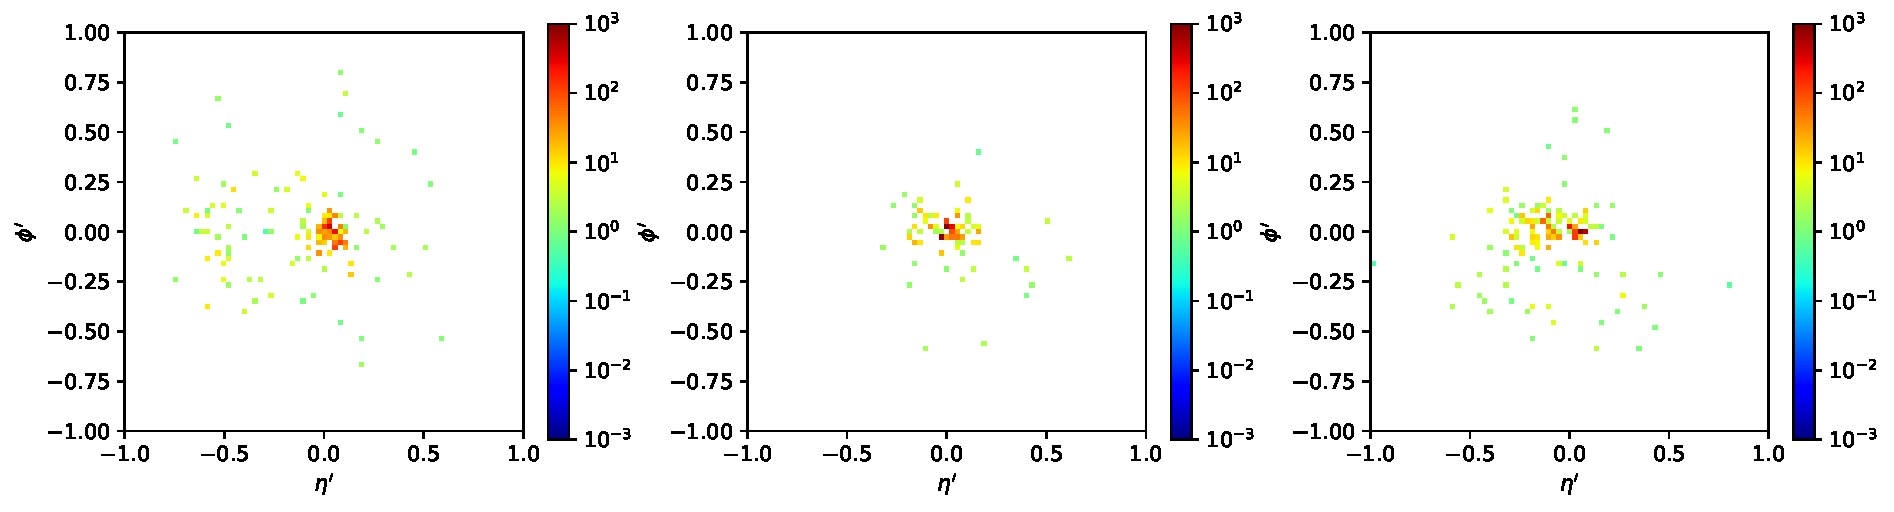
\includegraphics[width=0.95\textwidth]{HVmodel_jet_image_one_event_eta_phi_smearing.pdf}
            }
            \caption{The jet images before and after the $\eta-\phi$ smearing augmentation.}
            \label{fig:eta_phi_smearing_jet_constituent_jet_image}
        \end{figure}
        \begin{figure}[htpb]
            \centering
            \subfloat[Before augmentation]{
                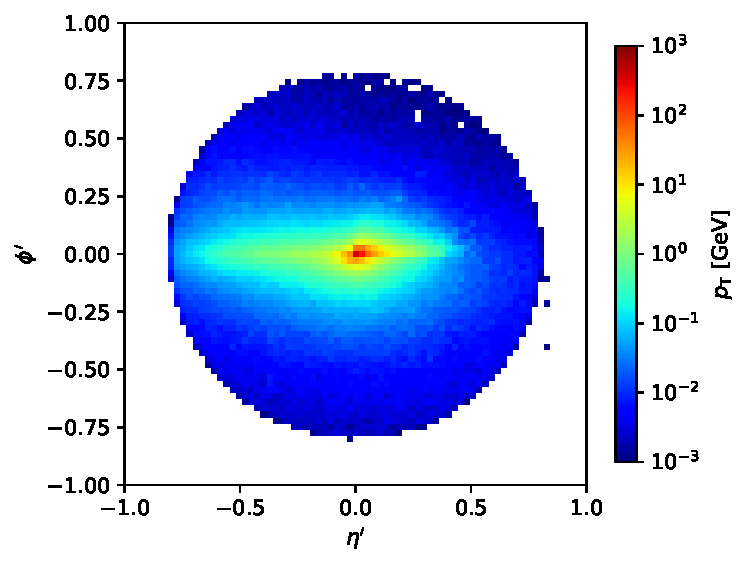
\includegraphics[width=0.45\textwidth]{HVmodel_jet_image_average_original.pdf}
            }
            \subfloat[After augmentation]{
                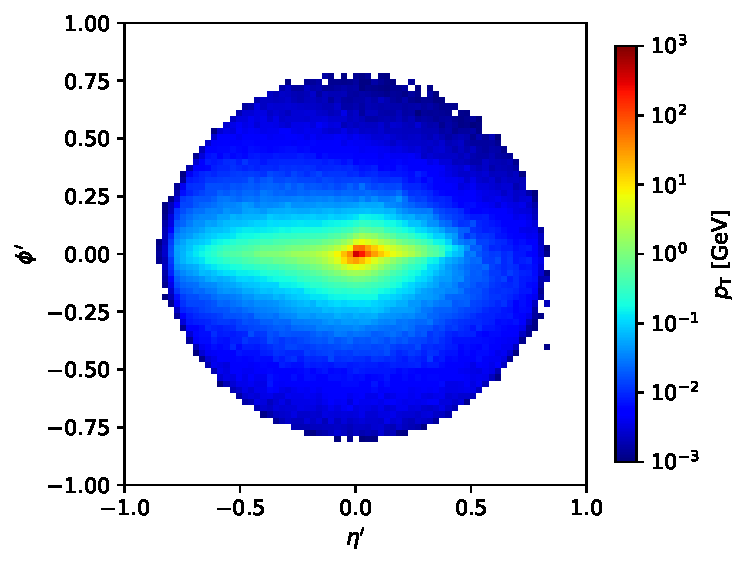
\includegraphics[width=0.45\textwidth]{HVmodel_jet_image_average_aug_1.pdf}
            }
            \caption{The average jet images before and after the $\eta-\phi$ smearing augmentation.}
            \label{fig:eta_phi_smearing_phi_jet_constituent_average_jet_image}
        \end{figure}

        We generate samples with sensitivity $S / \sqrt{B}$ ranging from 1 to 10. Then, apply the data augmentation to make larger samples. These samples are used for CNN training. Figure~\ref{fig:cwola_hunting_cnn_acc_data_augmetation} presents the training results. These numbers are evaluated from the pure samples. The ACC is better than previous results (blue curve in Figure~\ref{fig:cwola_hunting_cnn_acc}) for the ``+1 times'' curve for all sensitivities. The data augmentation technique suppresses the threshold and improves training performance.

        \begin{figure}[htpb]
            \centering
            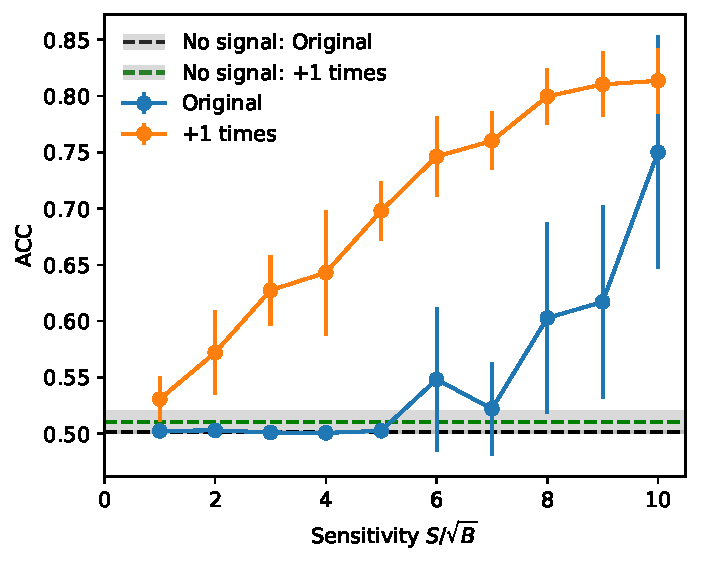
\includegraphics[width=0.55\textwidth]{HVmodel_CWoLa_CNN_aug_1.pdf}
            \caption{The performance of CWoLa CNN training as a function of the sensitivity. The error bar is the standard deviation of 10 times training. The grey band is the error bar of the ``without signal'' case.}
            \label{fig:cwola_hunting_cnn_acc_data_augmetation}
        \end{figure}

         Figure~\ref{fig:cwola_hunting_cnn_acc_data_augmetation_3_times} presents the training results with larger samples. For the ``+3 times'' curve, there is a strange result, the ACC is worse than the ``+1 times'' case for sensitivities $S / \sqrt{B} \ge 3$. Here are some things that could be improved in the training procedure, e.g. overfitting.
        \begin{figure}[htpb]
            \centering
            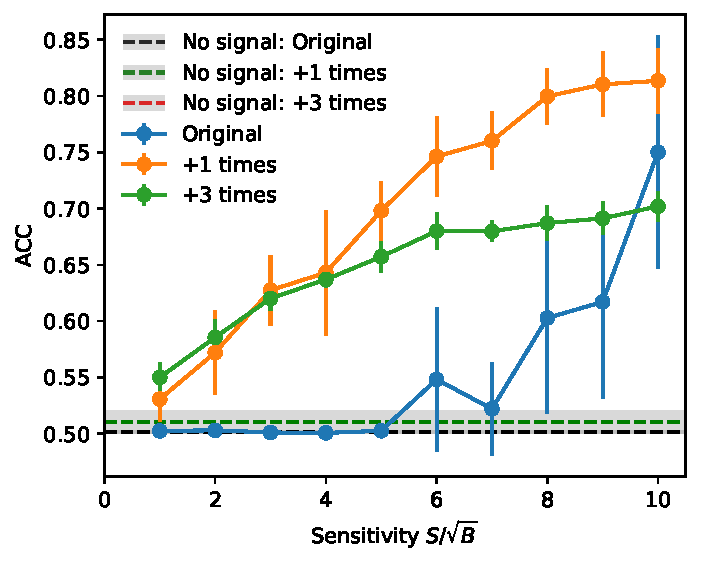
\includegraphics[width=0.55\textwidth]{HVmodel_CWoLa_CNN_aug_1_3.pdf}
            \caption{The performance of CWoLa CNN training as a function of the sensitivity. The error bar is the standard deviation of 10 times training. The grey band is the error bar of the ``without signal'' case.}
            \label{fig:cwola_hunting_cnn_acc_data_augmetation_3_times}
        \end{figure}

         Figure~\ref{fig:eta_phi_smearing_phi_jet_constituent_average_jet_image_aug_1_3} shows the average jet image for different augmentation times.
         \begin{figure}[htpb]
            \centering
            \subfloat[+1 times]{
                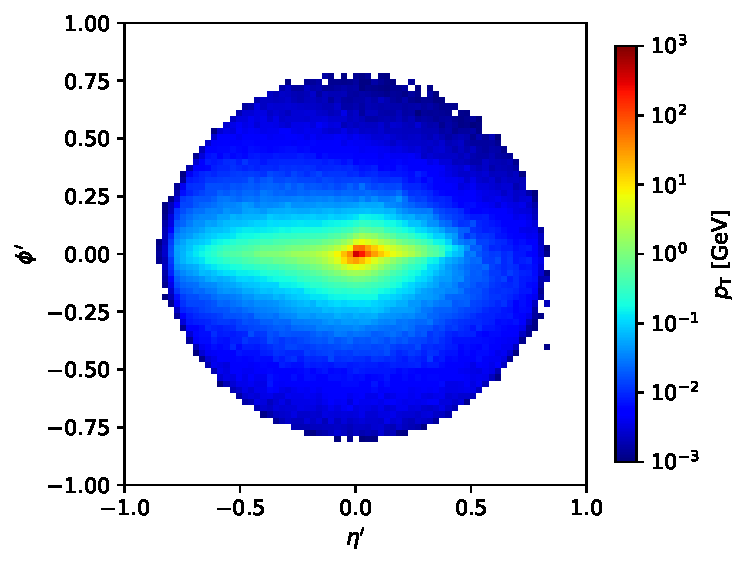
\includegraphics[width=0.45\textwidth]{HVmodel_jet_image_average_aug_1.pdf}
            }
            \subfloat[+3 times]{
                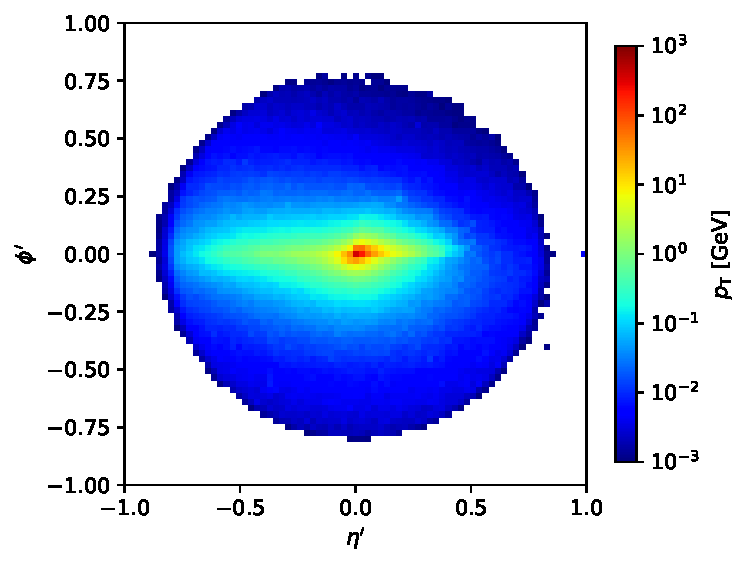
\includegraphics[width=0.45\textwidth]{HVmodel_jet_image_average_aug_3.pdf}
            }
            \caption{The average jet images of the $\eta-\phi$ smearing augmentation with different times.}
            \label{fig:eta_phi_smearing_phi_jet_constituent_average_jet_image_aug_1_3}
        \end{figure}
    % subsection data_augmentation (end)
    \subsection{Enlarge the training sample size}% (fold)
    \label{sub:enlarge_the_training_sample_size}
        To validate the correctness of the data augmentation results, we generated larger samples by scaling the luminosity. To compare the results with ``+1 times'' augmentation, we scale the luminosity to $\mathcal{L} = 139 \times 2 \text{ fb}^{-1}$. It is important to note that the number of signal events is not equal for ``+1 times'' and ``luminosity $\times 2$'' at the same sensitivity because the number of signal events is computed from $S / \sqrt{B}$ for a given $B$, resulting in the number of ``+1 times'' signal sample is greater by a factor of $\sqrt{2}$. Table~\ref{tab:training_sample_size_cwola_hunting_hv_aug_1_x2_luminosity} is an example. For a fair comparison, where the sizes of signal and background events are the same, we should compare the ``+1 times'' results with the point on the ``luminosity $\times 2$'' curve corresponding to $\sqrt{2}$ times the sensitivity.

        \begin{table}[htpb]
            \centering
            \caption{The training sample size for the original, ``+1 times'' and ``luminosity $\times 2$'' mixed sample. We set sensitivity $S / \sqrt{B} = 1$ in the signal region and evaluate the number of events in the signal region.}
            \label{tab:training_sample_size_cwola_hunting_hv_aug_1_x2_luminosity}

            \begin{tabular}{c|cc|cc|cc}
                                & \multicolumn{2}{c|}{Original}& \multicolumn{2}{c|}{+1 times}& \multicolumn{2}{c}{luminosity $\times 2$} \\
                Mixed sample    & Signal      & Background     & Signal      & Background     & Signal            & Background            \\ \hline
                Signal region   & 138         & 19k            & 276         & 38k            & 194               & 38k                   \\
                Sideband region & 40          & 29k            & 80          & 58k            & 56                & 58k
            \end{tabular}
        \end{table}

        Figure~\ref{fig:cwola_hunting_cnn_acc_x2_luminosity} presents the training results with larger samples. The results of ``luminosity $\times 2$'' is better than the original sample, but still worse than the ``+1 times'' case. Even considering the $\sqrt{2}$ scale factor, the corresponding points' performance is still worse. There may be something wrong with the data processing or training codes.
        \begin{figure}[htpb]
            \centering
            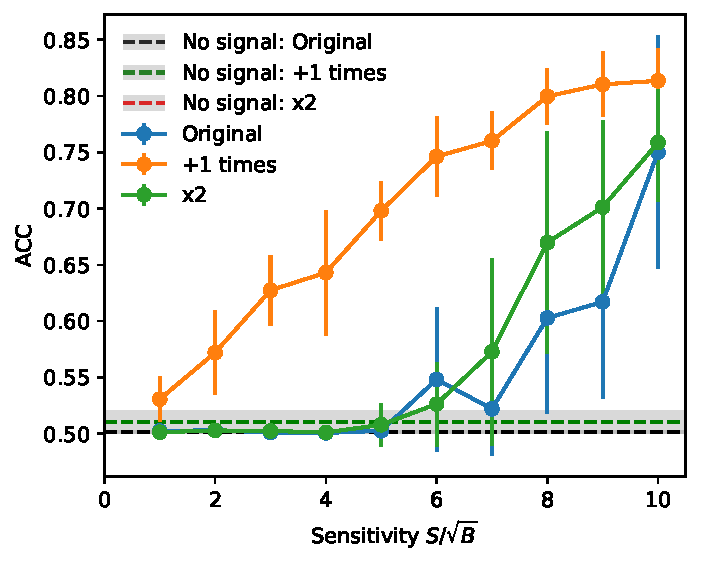
\includegraphics[width=0.55\textwidth]{HVmodel_CWoLa_CNN_aug_1_x2.pdf}
            \caption{The performance of CWoLa CNN training as a function of the sensitivity. The error bar is the standard deviation of 10 times training. The grey band is the error bar of the ``without signal'' case.}
            \label{fig:cwola_hunting_cnn_acc_x2_luminosity}
        \end{figure}
    % subsection enlarge_the_training_sample_size (end)
    \subsection{Check the codes and make more plots}% (fold)
    \label{sub:check_the_codes_and_make_more_plots}
        The data process steps from 2 to 5 (Section~\ref{sub:data_process_procedure}) have been checked and samples are processed again.

        Figure~\ref{fig:jet_constituent_pt_distribution} is the $p_\text{T}$ distribution of the jet constituents. The distributions of leading and sub-leading jet constituents are similar.
        \begin{figure}[htpb]
            \centering
            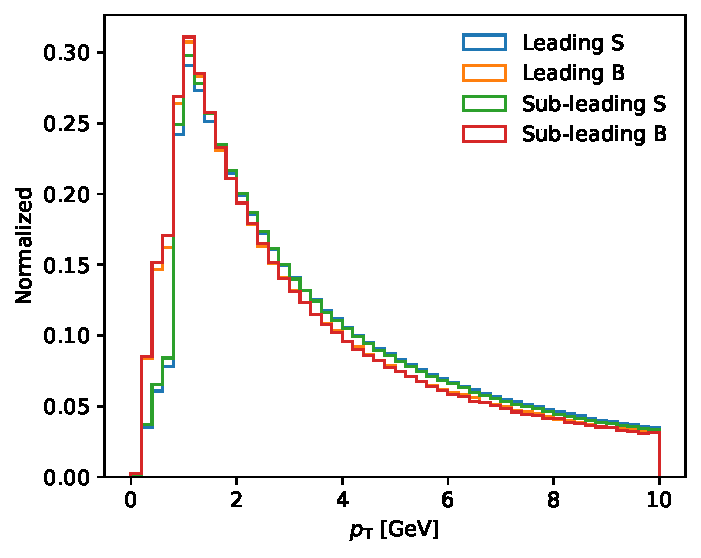
\includegraphics[width=0.55\textwidth]{hv_model_pt_distribution.pdf}
            \caption{The transverse momentum distribution of jet constituents.}
            \label{fig:jet_constituent_pt_distribution}
        \end{figure}

        Figure~\ref{fig:jet_constituent_eta_distribution} and \ref{fig:jet_constituent_phi_distribution} are the $\eta, \phi$ distributions before and after the augmentation. Because the smearing scale is small, the distributions look almost the same for both cases.

        \begin{figure}[htpb]
            \centering
            \subfloat[Leading Higgs]{
                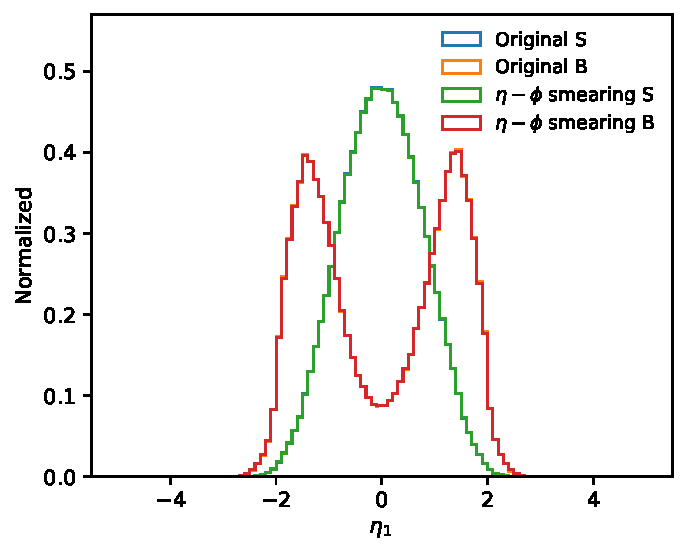
\includegraphics[width=0.45\textwidth]{hv_model_eta1_distribution_eta_phi_smearing.pdf}
            }
            \subfloat[Sub-leading Higgs]{
                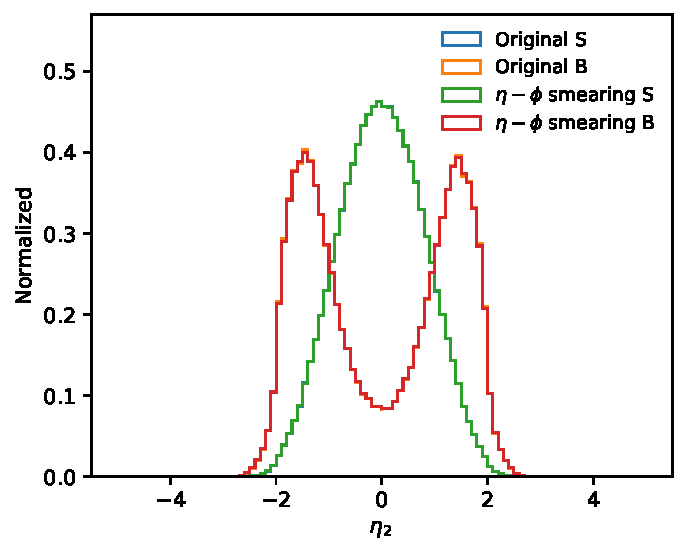
\includegraphics[width=0.45\textwidth]{hv_model_eta2_distribution_eta_phi_smearing.pdf}
            }
            \caption{The pseudorapidity distribution before and after the $\eta-\phi$ smearing augmentation. $\eta_1$ and $\eta_2$ are the pseudorapidities of the leading and sub-leading jet constituents.}
            \label{fig:jet_constituent_eta_distribution}
        \end{figure}
        \begin{figure}[htpb]
            \centering
            \subfloat[Leading Higgs]{
                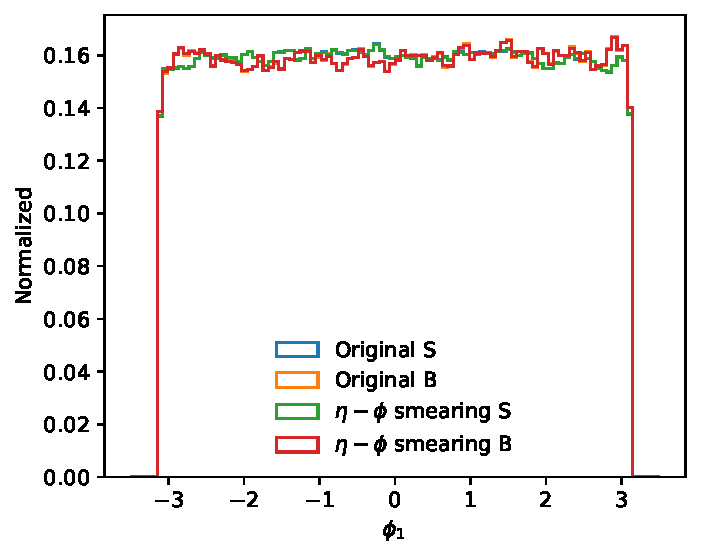
\includegraphics[width=0.45\textwidth]{hv_model_phi1_distribution_eta_phi_smearing.pdf}
            }
            \subfloat[Sub-leading Higgs]{
                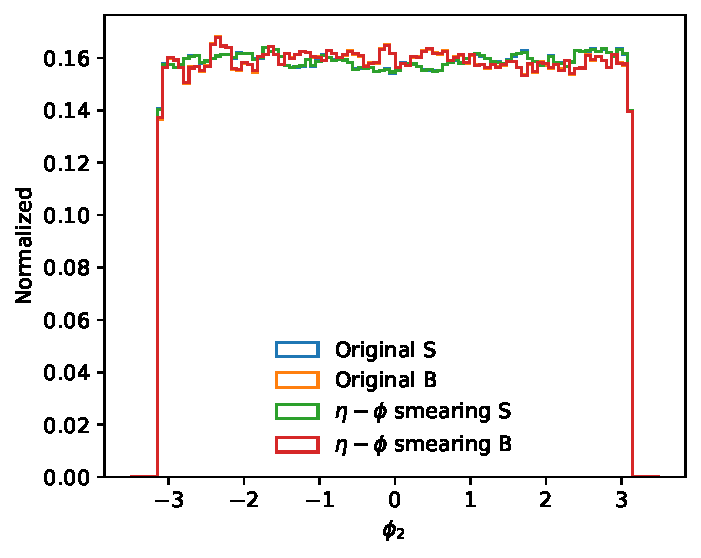
\includegraphics[width=0.45\textwidth]{hv_model_phi2_distribution_eta_phi_smearing.pdf}
            }
            \caption{The azimuthal angle distribution before and after the $\eta-\phi$ smearing augmentation. $\phi_1$ and $\phi_2$ are the azimuthal angles of the leading and sub-leading jet constituents.}
            \label{fig:jet_constituent_phi_distribution}
        \end{figure}

        Figure~\ref{fig:jet_constituent_average_jet_image_aug_1_x2} shows the average jet image for various cases.
        \begin{figure}[htpb]
            \centering
            \subfloat[Original]{
                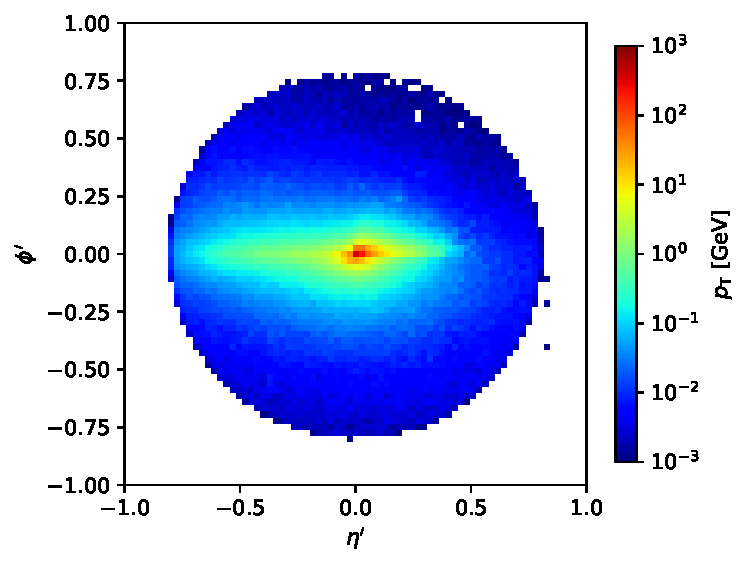
\includegraphics[width=0.31\textwidth]{HVmodel_jet_image_average_original.pdf}
            }
            \subfloat[+1 times augmentation]{
                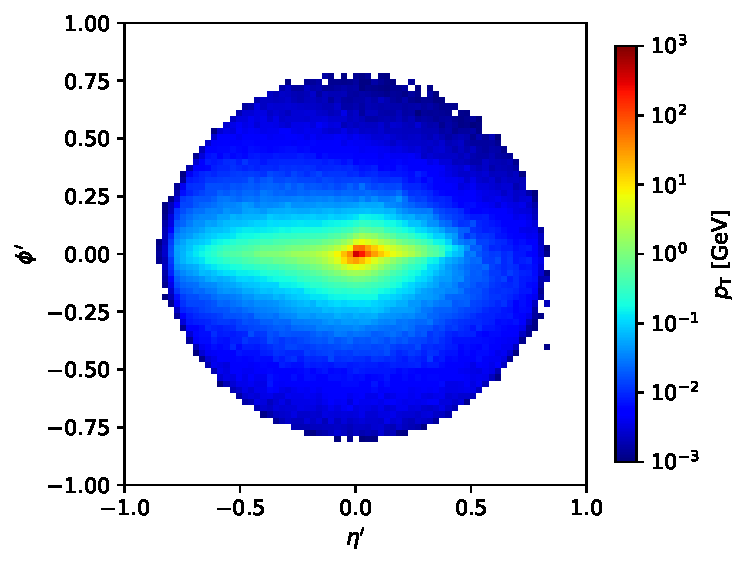
\includegraphics[width=0.31\textwidth]{HVmodel_jet_image_average_aug_1.pdf}
            }
            \subfloat[Luminosity $\times 2$]{
                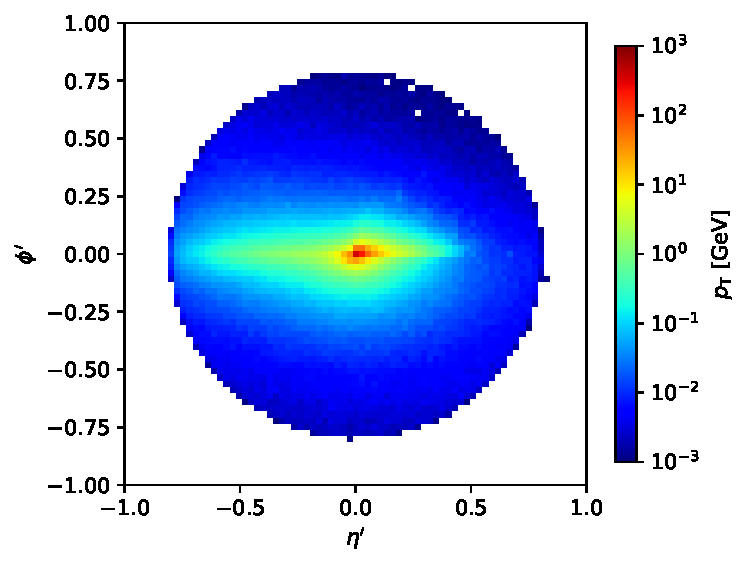
\includegraphics[width=0.31\textwidth]{HVmodel_jet_image_average_x2.pdf}
            }
            \caption{The average jet images of different cases. These plots are made from mixed samples.}
            \label{fig:jet_constituent_average_jet_image_aug_1_x2}
        \end{figure}

        Figure~\ref{fig:cwola_hunting_cnn_acc_x2_luminosity_re-processed_sample} is training results with re-processed samples.
        \begin{figure}[htpb]
            \centering
            \includegraphics[width=0.55\textwidth]{HVmodel_CWoLa_CNN_aug_1_x2_re-process.pdf}
            \caption{The performance of CWoLa CNN training with re-processed samples. The error bar is the standard deviation of 10 times training. The grey band is the error bar of the ``without signal'' case.}
            \label{fig:cwola_hunting_cnn_acc_x2_luminosity_re-processed_sample}
        \end{figure}
    % subsection check_the_codes_and_make_more_plots (end)
    \subsection{Sensitivity difference}% (fold)
    \label{sub:sensitivity_difference}
        The CWoLa CNN is applied for event selection. The threshold is set for a given background efficiency $\varepsilon_{\text{b}}$ (false positive rate). For a given $\varepsilon_b$, the sensitivity would be scale by a factor ${\varepsilon_\text{s}} / {\sqrt{\varepsilon_{\text{b}}}}$.

        Figure~\ref{fig:sensitivity_improvement_origin_aug_1_x2} is the sensitivity improvement of orginal, ``+1 times'' and ``luminosity $\times 2$'' samples. The $10\%$ curves give more stable results. The lower background efficiencies could achieve better results at the range with higher sensitivities, but the standard deviation would be much larger. Figure~\ref{fig:sensitivity_improvement_bkg_eff_01} compares the sensitivity improvement of various training samples with the same background efficiency. The ``+1 times'' samples provide the best threshold among all.

        \begin{figure}[htpb]
            \centering
            \subfloat[Original]{
                \includegraphics[width=0.31\textwidth]{HVmodel_sensitivity_improvement_original.pdf}
            }
            \subfloat[+1 times augmentation]{
                \includegraphics[width=0.31\textwidth]{HVmodel_sensitivity_improvement_aug_1.pdf}
            }
            \subfloat[Luminosity $\times 2$]{
                \includegraphics[width=0.31\textwidth]{HVmodel_sensitivity_improvement_x2.pdf}
            }
            \caption{The sensitivities before and after the CWoLa CNN selection. The thresholds are chosen from $\varepsilon_{\text{b}} = 10\%, 1\%, 0.1\%$. The slope of the dashed line is $1$, representing the same performance before and after the selection. The error bar is the standard deviation of 10 times training.}
            \label{fig:sensitivity_improvement_origin_aug_1_x2}
        \end{figure}

        \begin{figure}[htpb]
            \centering
            \includegraphics[width=0.55\textwidth]{HVmodel_sensitivity_improvement_bkg_eff_10.pdf}
            \caption{The sensitivities before and after the CWoLa CNN selection. The threshold is chosen from $\varepsilon_{\text{b}} = 10\%$. The slope of the dashed line is $1$, representing the same performance before and after the selection. The error bar is the standard deviation of 10 times training. The ``+1 times'' samples provide the best threshold.}
            \label{fig:sensitivity_improvement_bkg_eff_01}
        \end{figure}
    % subsection sensitivity_difference (end)
    \subsection{Training and true performance}% (fold)
    \label{sub:training_and_true_performance}
        In our intuition, we would expect that``+1 times'' and ``luminosity  $\times 2$'' samples should exhibit similar performance, or the ``luminosity  $\times 2$'' sample might provide better results since the data augmentation generates more samples from the known data. However, the results in Figure~\ref{fig:sensitivity_improvement_bkg_eff_01} contradict our intuition. Since we use the CWoLa approach, our comparison is not based on the training performance on mixed samples; instead, we evaluate the testing performance on pure samples, referred to as ``true performance.'' The relationship between training and true performance may not be a monotonic function and can be complicated.

        Figure~\ref{fig:training_and_true_acc_ori_aug_1_x2} is the scatter plot for training and true accuracy. Training ACC values are close for all cases, but true ACC values can differ greatly. The true ACC is ten times larger than the training ACC range. For training ACC, both ``+1 times'' and ``luminosity $\times 2$'' samples show similar performance, slightly better than the original results. For the true ACC, the ``+1 times'' provides much better results. It seems that ``+1 times'' samples are more effective in improving true ACC.
        \begin{figure}[htpb]
            \centering
            \includegraphics[width=0.55\textwidth]{HVmodel_training_true_acc_aug_1_x2.pdf}
            \caption{Scatter plot for training ACC and true ACC. The slope of the grey dashed line is $1$, representing the same training and true ACC. The range of training ACC is tiny, roughly 0.03, while the range of true ACC is about 0.3.}
            \label{fig:training_and_true_acc_ori_aug_1_x2}
        \end{figure}

        Figure~\ref{fig:training_and_true_acc_ori_aug_1_3_x2} includes results with``+3 times'' training . The ``+3 times'' samples provide much better training ACC but do not achieve higher performance for true ACC.
        \begin{figure}[htpb]
            \centering
            \includegraphics[width=0.55\textwidth]{HVmodel_training_true_acc_aug_1_3_x2.pdf}
            \caption{Scatter plot for training ACC and true ACC. The slope of the grey dashed line is $1$, representing the same training and true ACC.}
            \label{fig:training_and_true_acc_ori_aug_1_3_x2}
        \end{figure}
    % subsection training_and_true_performance (end)
    \subsection{Miscellaneous test}% (fold)
    \label{sub:miscellaneous_test}
        \subsubsection{Sensitivity 11 to 20}% (fold)
        \label{subs:sensitivity_11_to_20}
            To find out the training performance when sensitivity is greater than 10, we generate the samples with sensitivity ranging from 11 to 20. The training performance is summarized in Figure~\ref{fig:cwola_cnn_training_performance_11_20}. The ACC is increased when the sensitivity is increased. When the $S / \sqrt{B} > 13$, the ACC improvement is slowed, where the ACC is 85\%. The training ACC is still similar for all cases, but the true ACC exhibits a better value when the sensitivity is higher.
            \begin{figure}[htpb]
                \centering
                \subfloat[]{
                    \includegraphics[width=0.45\textwidth]{HVmodel_CWoLa_CNN_sensitivity_11_20.pdf}
                }
                \subfloat[]{
                    \includegraphics[width=0.45\textwidth]{HVmodel_training_true_acc_sensitivity_11_20.pdf}
                }
                \caption{(a) The performance of CWoLa CNN training with higher sensitivity samples. The error bar is the standard deviation of 10 times training. The grey band is the error bar of the ``without signal'' case. (b) Scatter plot for training ACC and true ACC. The slope of the grey dashed line is 1, representing the same training and true ACC.}
                \label{fig:cwola_cnn_training_performance_11_20}
            \end{figure}
        % subsubsection sensitivity_11_to_20 (end)
        \subsubsection{+1 copy sample}% (fold)
        \label{subs:_1_copy_sample}
            To investigate the impact of the data augmentation technique, we generate a sample by duplicating the original sample without any augmentation. This sample is called ``+1 copy.''
            Figure~\ref{fig:cwola_cnn_training_performance_copy_1} is the ACC curve and ACC distribution. The ACC is close to the ``+1 augmentation'' case when $S / \sqrt{B} \le 4$, while the ACC is worse when $S / \sqrt{B} \ge 5$. The training ACC is much better than the original and ``+1 augmentation'' samples, but the true ACC can not achieve higher values.
            \begin{figure}[htpb]
                \centering
                \subfloat[]{
                    \includegraphics[width=0.45\textwidth]{HVmodel_CWoLa_CNN_aug_1_copy_1.pdf}
                }
                \subfloat[]{
                    \includegraphics[width=0.45\textwidth]{HVmodel_training_true_acc_aug_1_copy_1.pdf}
                }
                \caption{(a) The performance of CWoLa CNN training with ``+1 copy'' samples. The error bar is the standard deviation of 10 times training. The grey band is the error bar of the ``without signal'' case. (b) Scatter plot for training ACC and true ACC. The slope of the grey dashed line is 1, representing the same training and true ACC.}
                \label{fig:cwola_cnn_training_performance_copy_1}
            \end{figure}

            Figure~\ref{fig:sensitivity_improvement_bkg_eff_01_copy_1} is the sensitivity improvement. The performance of the ``+1 copy'' sample is worse than ``+1 augmentation''. It exhibits the worst results in high-sensitivity regions. The data augmentation is effective in improving the true ACC.
            \begin{figure}[htpb]
                \centering
                \includegraphics[width=0.55\textwidth]{HVmodel_sensitivity_improvement_bkg_eff_10_copy_1.pdf}
                \caption{The sensitivities before and after the CWoLa CNN selection. The threshold is chosen from $\varepsilon_{\text{b}} = 10\%$. The slope of the dashed grey line is $1$, representing the same performance before and after the selection. The error bar is the standard deviation of 10 times training. The ``+1 times'' samples provide the best threshold.}
                \label{fig:sensitivity_improvement_bkg_eff_01_copy_1}
            \end{figure}
        % subsubsection _1_copy_sample (end)
    % subsection miscellaneous_test (end)
    \subsection{Train on only augmented sample}% (fold)
    \label{sub:train_on_only_augmented_sample}
        We train the CWoLa CNN with only augmented datasets to diagnose augmented samples. The training samples are generated from the original dataset and only the augmented part is kept for training. We test ``1 augmentation'' and ``2 augmentation'' cases. They consist of pure augmented samples. Their sizes are 1 time and 2 times the original dataset.

        Figure~\ref{fig:cwola_cnn_training_performance_only_aug_1} shows the ACC curve and ACC distribution with the ``1 augmentation'' case. The ACC of the ``1 augmentation'' sample is better than the ``original'' one at $S / \sqrt{B}=7$, but they perform similarly on other sensitivities. Figure~\ref{fig:sensitivity_improvement_bkg_eff_01_only_aug_1} is the sensitivity improvement. The threshold of the ``1 augmentation'' sample is lower than the ``original'' one, but they exhibit similar performance on other sensitivities. These results are consistent with the ACC curve. The difference at $S / \sqrt{B}=7$ may come from the training fluctuation.
        \begin{figure}[htpb]
            \centering
            \subfloat[]{
                \includegraphics[width=0.45\textwidth]{HVmodel_CWoLa_CNN_only_aug_1.pdf}
            }
            \subfloat[]{
                \includegraphics[width=0.45\textwidth]{HVmodel_training_true_acc_only_aug_1.pdf}
            }
            \caption{(a) The performance of CWoLa CNN training with ``1 augmentation'' samples. The error bar is the standard deviation of 10 times training. The grey band is the error bar of the ``without signal'' case. (b) Scatter plot for training ACC and true ACC. The slope of the grey dashed line is 1, representing the same training and true ACC.}
            \label{fig:cwola_cnn_training_performance_only_aug_1}
        \end{figure}
        \begin{figure}[htpb]
            \centering
            \includegraphics[width=0.55\textwidth]{HVmodel_sensitivity_improvement_bkg_eff_10_only_aug_1.pdf}
            \caption{The sensitivities before and after the CWoLa CNN selection. The threshold is chosen from $\varepsilon_{\text{b}} = 10\%$. The slope of the dashed grey line is $1$, representing the same performance before and after the selection. The error bar is the standard deviation of 10 times training. The ``1 augmentation'' samples provide a lower threshold.}
            \label{fig:sensitivity_improvement_bkg_eff_01_only_aug_1}
        \end{figure}

        Figure~\ref{fig:cwola_cnn_training_performance_only_aug_2} is the training results with ``2 augmentation'' samples. The results are similar to the ``+1 augmentation'' case. Figure~\ref{fig:sensitivity_improvement_bkg_eff_01_only_aug_2} is the sensitivity improvement. The performance of the ``2 augmentation'' samples is almost the same as ``+1 augmentation''.
        \begin{figure}[htpb]
            \centering
            \subfloat[]{
                \includegraphics[width=0.45\textwidth]{HVmodel_CWoLa_CNN_only_aug_2.pdf}
            }
            \subfloat[]{
                \includegraphics[width=0.45\textwidth]{HVmodel_training_true_acc_only_aug_2.pdf}
            }
            \caption{(a) The performance of CWoLa CNN training with ``2 augmentation'' samples. The error bar is the standard deviation of 10 times training. The grey band is the error bar of the ``without signal'' case. (b) Scatter plot for training ACC and true ACC. The slope of the grey dashed line is 1, representing the same training and true ACC.}
            \label{fig:cwola_cnn_training_performance_only_aug_2}
        \end{figure}
        \begin{figure}[htpb]
            \centering
            \includegraphics[width=0.55\textwidth]{HVmodel_sensitivity_improvement_bkg_eff_10_only_aug_2.pdf}
            \caption{The sensitivities before and after the CWoLa CNN selection. The threshold is chosen from $\varepsilon_{\text{b}} = 10\%$. The slope of the dashed grey line is $1$, representing the same performance before and after the selection. The error bar is the standard deviation of 10 times training. The ``2 augmentation'' and ``+1 augmentation'' samples perform similarly.}
            \label{fig:sensitivity_improvement_bkg_eff_01_only_aug_2}
        \end{figure}
    % subsection train_on_only_augmented_sample (end)
    \subsection{Change the smearing scale}% (fold)
    \label{sub:change_the_smearing_scale}
        To investigate the impact of the smearing scale $\Lambda$ of data augmentation, we generate samples with various $\Lambda$ for CWoLa CNN training. We test $\Lambda = 200, 500 \text{ MeV}$ samples.

        Figure~\ref{fig:eta_phi_smearing_jet_constituent_jet_image_smearing_scale} and \ref{fig:eta_phi_smearing_phi_jet_constituent_average_jet_image_smearing_scale} are the jet image with different smearing scales. When the smearing scale increases the jet image is more different.
        \begin{figure}[htpb]
            \centering
            \subfloat[Original]{
                \includegraphics[width=0.95\textwidth]{HVmodel_jet_image_one_event_original.pdf}
            } \\
            \subfloat[$\Lambda = \text{100 MeV}$]{
                \includegraphics[width=0.95\textwidth]{HVmodel_jet_image_one_event_eta_phi_smearing.pdf}
            } \\
            \subfloat[$\Lambda = \text{200 MeV}$]{
                \includegraphics[width=0.95\textwidth]{HVmodel_jet_image_one_event_eta_phi_smearing_std_02.pdf}
            } \\
            \subfloat[$\Lambda = \text{500 MeV}$]{
                \includegraphics[width=0.95\textwidth]{HVmodel_jet_image_one_event_eta_phi_smearing_std_05.pdf}
            }
            \caption{The jet images with different smearing scale $\Lambda$.}
            \label{fig:eta_phi_smearing_jet_constituent_jet_image_smearing_scale}
        \end{figure}
        \begin{figure}[htpb]
            \centering
            \subfloat[Original]{
                \includegraphics[width=0.45\textwidth]{HVmodel_jet_image_average_original.pdf}
            }
            \subfloat[$\Lambda = \text{100 MeV}$]{
                \includegraphics[width=0.45\textwidth]{HVmodel_jet_image_average_aug_1.pdf}
            } \\
            \subfloat[$\Lambda = \text{200 MeV}$]{
                \includegraphics[width=0.45\textwidth]{HVmodel_jet_image_average_aug_1_std_02.pdf}
            }
            \subfloat[$\Lambda = \text{500 MeV}$]{
                \includegraphics[width=0.45\textwidth]{HVmodel_jet_image_average_aug_1_std_05.pdf}
            }
            \caption{The average jet images with different smearing scale $\Lambda$.}
            \label{fig:eta_phi_smearing_phi_jet_constituent_average_jet_image_smearing_scale}
        \end{figure}

        Figure~\ref{fig:cwola_cnn_training_performance_smearing_scale} is the training results with various smearing scales. In the low-sensitivity region, the performance is better for the lower smearing scale, while in the high-sensitivity region, the performance is better for the higher smearing scale. Figure~\ref{fig:sensitivity_improvement_bkg_eff_01_smearing_scale} is the sensitivity improvement. The results are consistent with the ACC curve. $\Lambda = \text{100 MeV}$ exhibits the lower threshold.
        \begin{figure}[htpb]
            \centering
            \subfloat[]{
                \includegraphics[width=0.45\textwidth]{HVmodel_CWoLa_CNN_aug_1_std_01_02_05.pdf}
            }
            \subfloat[]{
                \includegraphics[width=0.45\textwidth]{HVmodel_training_true_acc_aug_1_std_01_02_05.pdf}
            }
            \caption{(a) The performance of CWoLa CNN training with various smearing scales. The error bar is the standard deviation of 10 times training. The grey band is the error bar of the ``without signal'' case. ``+1'' means the +1 time augmentation sample. (b) Scatter plot for training ACC and true ACC. The slope of the grey dashed line is 1, representing the same training and true ACC.}
            \label{fig:cwola_cnn_training_performance_smearing_scale}
        \end{figure}
        \begin{figure}[htpb]
            \centering
            \includegraphics[width=0.55\textwidth]{HVmodel_sensitivity_improvement_bkg_eff_10_aug_1_std_01_02_05.pdf}
            \caption{The sensitivities before and after the CWoLa CNN selection. The threshold is chosen from $\varepsilon_{\text{b}} = 10\%$. The slope of the dashed grey line is $1$, representing the same performance before and after the selection. The error bar is the standard deviation of 10 times training. ``+1'' means the +1 time augmentation sample.}
            \label{fig:sensitivity_improvement_bkg_eff_01_smearing_scale}
        \end{figure}
    % subsection change_the_smearing_scale (end)
    \subsection{Duplicate training sample}% (fold)
    \label{sub:duplicate_training_sample}
        To compare the results with Section~\ref{subs:_1_copy_sample}, we generate a sample by duplicating the original without further shuffle. Therefore, the first $n$-th sample and $n+1$-th to the final sample should be the same. This dataset is called ``+1 copy without shuffle.'' Figure~\ref{fig:average_jet_image_0_to_n_n_to_2n} is the average jet image of the first $n$-th sample and $n+1$-th to the final sample. These two images are the same.
        \begin{figure}[htpb]
            \centering
            \subfloat[$1 \sim n$]{
                \includegraphics[width=0.45\textwidth]{HVmodel_jet_image_1_copy_0_to_n.pdf}
            }
            \subfloat[$n+1 \sim 2n$]{
                \includegraphics[width=0.45\textwidth]{HVmodel_jet_image_1_copy_n_to_2n.pdf}
            }
            \caption{The average jet image of first $n$-th sample and $n+1$-th to the final sample.}
            \label{fig:average_jet_image_0_to_n_n_to_2n}
        \end{figure}

        Figure~\ref{fig:cwola_cnn_training_performance_copy_1_wo_shuffle} is the ACC curve and ACC distribution. The training results for ``+1 copy'' and ``+1 copy without shuffle'' do not have significant differences and they all perform better than the original training sample.
        \begin{figure}[htpb]
            \centering
            \subfloat[]{
                \includegraphics[width=0.45\textwidth]{HVmodel_CWoLa_CNN_copy_1_wo_shuffle.pdf}
            }
            \subfloat[]{
                \includegraphics[width=0.45\textwidth]{HVmodel_training_true_acc_copy_1_wo_shuffle.pdf}
            }
            \caption{(a) The performance of CWoLa CNN training with ``+1 copy'' and ``+1 copy without shuffle'' samples. The error bar is the standard deviation of 10 times training. The grey band is the error bar of the ``without signal'' case. (b) Scatter plot for training ACC and true ACC. The slope of the grey dashed line is 1, representing the same training and true ACC.}
            \label{fig:cwola_cnn_training_performance_copy_1_wo_shuffle}
        \end{figure}

        Figure~\ref{fig:sensitivity_improvement_bkg_eff_01_copy_1_wo_shuffle} is the sensitivity improvement. The performance of the ``+1 copy'' and ``+1 copy without shuffle'' samples are similar.
        \begin{figure}[htpb]
            \centering
            \includegraphics[width=0.55\textwidth]{HVmodel_sensitivity_improvement_bkg_eff_10_copy_1_wo_shuffle.pdf}
            \caption{The sensitivities before and after the CWoLa CNN selection. The threshold is chosen from $\varepsilon_{\text{b}} = 10\%$. The slope of the dashed grey line is $1$, representing the same performance before and after the selection. The error bar is the standard deviation of 10 times training.}
            \label{fig:sensitivity_improvement_bkg_eff_01_copy_1_wo_shuffle}
        \end{figure}

        \subsubsection{Remove shuffle in training code}% (fold)
        \label{subs:remove_shuffle_in_training_code}
            I remove default shuffles in the training codes. In the default setting, the training sample would be shuffled before training and testing sample splitting and each epoch training. Figure~\ref{fig:cwola_cnn_training_performance_copy_1_wo_shuffle_code} is the ACC curve and ACC distribution. The training results of removing shuffling codes are similar to the previous one, and all ``+1 copy'' samples perform better than the original.
            \begin{figure}[htpb]
                \centering
                \subfloat[]{
                    \includegraphics[width=0.45\textwidth]{HVmodel_CWoLa_CNN_copy_1_wo_shuffle_code.pdf}
                }
                \subfloat[]{
                    \includegraphics[width=0.45\textwidth]{HVmodel_training_true_acc_copy_1_wo_shuffle_code.pdf}
                }
                \caption{(a) The performance of CWoLa CNN training with ``+1 copy'' sample and ``+1 copy'' with removing shuffling codes. The error bar is the standard deviation of 10 times training. The grey band is the error bar of the ``without signal'' case. (b) Scatter plot for training ACC and true ACC. The slope of the grey dashed line is 1, representing the same training and true ACC.}
                \label{fig:cwola_cnn_training_performance_copy_1_wo_shuffle_code}
            \end{figure}

            Figure~\ref{fig:sensitivity_improvement_bkg_eff_01_copy_1_wo_shuffle_code} is the sensitivity improvement. The performance of the ``+1 copy'' sample and ``+1 copy'' with removing shuffling codes are similar.
            \begin{figure}[htpb]
                \centering
                \includegraphics[width=0.55\textwidth]{HVmodel_sensitivity_improvement_bkg_eff_10_copy_1_wo_shuffle_code.pdf}
                \caption{The sensitivities before and after the CWoLa CNN selection. The threshold is chosen from $\varepsilon_{\text{b}} = 10\%$. The slope of the dashed grey line is $1$, representing the same performance before and after the selection. The error bar is the standard deviation of 10 times training.}
                \label{fig:sensitivity_improvement_bkg_eff_01_copy_1_wo_shuffle_code}
            \end{figure}
        % subsubsection remove_shuffle_in_training_code (end)
        \subsubsection{Half original + copy}% (fold)
        \label{subs:half_original_copy}
            To make sure the better training results come from adding copy samples and not from the sample size, we use half the original sample and duplicate it. This dataset is called `` half +1 copy'' and has the same size as the original sample.

            Figure~\ref{fig:cwola_cnn_training_performance_half_copy_1} is the ACC curve and ACC distribution. The training results of ``half +1 copy'' are better than the original training sample in the low sensitivity region, while in the high sensitivity region, ``half +1 copy'' has the worse results. For the ``half +1 copy'' case, the training ACC is overfitting when $S / \sqrt{B} \ge 6$.
            \begin{figure}[htpb]
                \centering
                \subfloat[]{
                    \includegraphics[width=0.45\textwidth]{HVmodel_CWoLa_CNN_half_copy_1.pdf}
                }
                \subfloat[]{
                    \includegraphics[width=0.45\textwidth]{HVmodel_training_true_acc_half_copy_1.pdf}
                }
                \caption{(a) The performance of CWoLa CNN training with ``+1 copy'' sample and ``half +1 copy'' datasets. The error bar is the standard deviation of 10 times training. The grey band is the error bar of the ``without signal'' case. (b) Scatter plot for training ACC and true ACC. The slope of the grey dashed line is 1, representing the same training and true ACC.}
                \label{fig:cwola_cnn_training_performance_half_copy_1}
            \end{figure}

            Figure~\ref{fig:sensitivity_improvement_bkg_eff_01_half_copy_1} is the sensitivity improvement. The threshold of the ``half +1 copy'' sample is lower than the original training sample, but the sensitivity improvement is smaller than the original dataset in the high sensitivity region.
            \begin{figure}[htpb]
                \centering
                \includegraphics[width=0.55\textwidth]{HVmodel_sensitivity_improvement_bkg_eff_10_half_copy_1.pdf}
                \caption{The sensitivities before and after the CWoLa CNN selection. The threshold is chosen from $\varepsilon_{\text{b}} = 10\%$. The slope of the dashed grey line is $1$, representing the same performance before and after the selection. The error bar is the standard deviation of 10 times training.}
                \label{fig:sensitivity_improvement_bkg_eff_01_half_copy_1}
            \end{figure}
        % subsubsection half_original_copy (end)
    % subsection duplicate_training_sample (end)
    \subsection{Another testing dataset}% (fold)
    \label{sub:another_testing_dataset}
        To rule out the problem in testing samples, I generate more signal and background samples and prepare another testing dataset. The testing results of old and new testing samples are shown in Figure~\ref{fig:acc_curve_two_testing_sample}. All cases perform similarly on two testing datasets. Note that because we only save the best model, we only present the ACC with the best training model for each case.
        \begin{figure}[htpb]
            \centering
            \subfloat[Original]{
                \includegraphics[width=0.31\textwidth]{HVmodel_CWoLa_CNN_new_testing_sample.pdf}
            }
            \subfloat[+1 time augmatation]{
                \includegraphics[width=0.31\textwidth]{HVmodel_CWoLa_CNN_aug_1_new_testing_sample.pdf}
            }
            \subfloat[Luminosity $\times 2$]{
                \includegraphics[width=0.31\textwidth]{HVmodel_CWoLa_CNN_x2_new_testing_sample.pdf}
            } \\
            \subfloat[+1 time copy]{
                \includegraphics[width=0.31\textwidth]{HVmodel_CWoLa_CNN_copy_1_new_testing_sample.pdf}
            }
            \subfloat[1 time augmatation]{
                \includegraphics[width=0.31\textwidth]{HVmodel_CWoLa_CNN_only_aug_1_new_testing_sample.pdf}
            }
            \subfloat[half + 1 time copy]{
                \includegraphics[width=0.31\textwidth]{HVmodel_CWoLa_CNN_half_copy_1_new_testing_sample.pdf}
            }
            \caption{The accuracy curves of two different testing sets. We present the accuracy of the best training model. In all cases, they have similar performance.}
            \label{fig:acc_curve_two_testing_sample}
        \end{figure}
    % subsection another_testing_dataset (end)
    \subsection{Original + \texorpdfstring{$x$}{x} Copy}% (fold)
    \label{sub:original_x_copy}
        The training datasets with different ratios of duplicated samples are generated. The training dataset consists of the original sample and $x$ copy sample, where ratio $x=$ 0.25, 0.50, 0.75. Figure~\ref{fig:cwola_cnn_training_performance_copy_ratio} is the ACC curve and ACC distribution. The training results of dataset adding copy samples are better than the original training sample in the low sensitivity region. The training results differ for $x = 0.50, 0.75$ when $S / \sqrt{B} \ge 6$. From the ACC scatter plot, the model seems to be over-training in this region.
        \begin{figure}[htpb]
            \centering
            \subfloat[]{
                \includegraphics[width=0.45\textwidth]{HVmodel_CWoLa_CNN_copy_ratio.pdf}
            }
            \subfloat[]{
                \includegraphics[width=0.45\textwidth]{HVmodel_training_true_acc_copy_ratio.pdf}
            }
            \caption{(a) The performance of CWoLa CNN training with various copy ratio datasets. The error bar is the standard deviation of 10 times training. The grey band is the error bar of the ``without signal'' case. (b) Scatter plot for training ACC and true ACC. The slope of the grey dashed line is 1, representing the same training and true ACC.}
            \label{fig:cwola_cnn_training_performance_copy_ratio}
        \end{figure}

        Figure~\ref{fig:sensitivity_improvement_bkg_eff_copy_ratio} is the sensitivity improvement. For $\varepsilon_{\text{b}} = 10\%$, the $+0.50 \sim +1$ copy samples have similar thresholds lower than the original training sample. Still, the sensitivity improvement is smaller than the original dataset in the high-sensitivity region. When the background efficiency is lower, the $+ 0.50$ copy and $+ 0.75$ copy samples perform better than other cases, even though they are over-training.
        \begin{figure}[htpb]
            \centering
            \includegraphics[width=0.97\textwidth]{HVmodel_sensitivity_improvement_bkg_eff_copy_ratio.pdf}
            \caption{The sensitivities before and after the CWoLa CNN selection. The thresholds are chosen from $\varepsilon_{\text{b}} = 10\%, 1\%, 0.1\%$. The slope of the dashed grey line is $1$, representing the same performance before and after the selection. The error bar is the standard deviation of 10 times training.}
            \label{fig:sensitivity_improvement_bkg_eff_copy_ratio}
        \end{figure}
    % subsection original_x_copy (end)
    \subsection{Remove rectification}% (fold)
    \label{sub:remove_rectification}
        For a properly constructed classifier, its accuracies should be greater than 50\% or it just mislabels the signal and background events.    Thus, a couple of codes are used for swapping labels. However, if the dataset causes a larger standard deviation, the swapping procedure might make a fake improvement. To investigate the impact of the ``rectification'', we remove the code that changes labels and train the CWoLa CNN again. We test on the original, ``luminosity $\times 2$'' and ``+1 copy'' datasets. The relabeling process before evaluating the ACC and sensitivity improvement is commented out.

        Figure~\ref{fig:acc_curve_w_wo_swap_label} is accuracy curves with different training datasets. Figure~\ref{fig:acc_scatter_w_wo_swap_label} is an accuracy scatter plot with various training datasets. The training results with and without swapping procedures are similar for all cases. It seems that the rectification process does not greatly impact the performance. The rectification is not the main reason for the improvement.
        \begin{figure}[htpb]
            \centering
            \subfloat[Original]{
                \includegraphics[width=0.31\textwidth]{HVmodel_CWoLa_CNN_origin_no_swap.pdf}
            }
            \subfloat[Luminosity $\times 2$]{
                \includegraphics[width=0.31\textwidth]{HVmodel_CWoLa_CNN_x2_no_swap.pdf}
            }
            \subfloat[+1 time copy]{
                \includegraphics[width=0.31\textwidth]{HVmodel_CWoLa_CNN_copy_1_no_swap.pdf}
            }
            \caption{The accuracy curves with and without the rectification procedure. The error bar is the standard deviation of 10 times training. The grey band is the error bar of the ``without signal'' case.}
            \label{fig:acc_curve_w_wo_swap_label}
        \end{figure}
        \begin{figure}[htpb]
            \centering
            \subfloat[Original]{
                \includegraphics[width=0.31\textwidth]{HVmodel_training_true_acc_origin_no_swap.pdf}
            }
            \subfloat[Luminosity $\times 2$]{
                \includegraphics[width=0.31\textwidth]{HVmodel_training_true_acc_x2_no_swap.pdf}
            }
            \subfloat[+1 time copy]{
                \includegraphics[width=0.31\textwidth]{HVmodel_training_true_acc_copy_1_no_swap.pdf}
            }
            \caption{Scatter plots for training ACC and true ACC with and without the rectification procedure. The slope of the grey dashed line is 1, representing the same training and true ACC.}
            \label{fig:acc_scatter_w_wo_swap_label}
        \end{figure}

        Figure~\ref{fig:sensitivity_improvement_bkg_eff_no_swap} is the sensitivity improvement. The training results with and without swapping procedures are similar for all cases. These results are consistent with the results of accuracy curves. The ``+1 copy'' dataset has the lowest threshold which is between 3 and 4 when $\varepsilon_{\text{b}} = 10\%$, but the sensitivity improvement is smaller than the original and ``luminosity $\times 2$'' datasets in the high sensitivity region. The ``luminosity $\times 2$'' threshold is lower than the original sample but higher than the ``+1 copy'' dataset.
        \begin{figure}[htpb]
            \centering
            \includegraphics[width=0.97\textwidth]{HVmodel_sensitivity_improvement_bkg_eff_copy_1_no_swap.pdf}
            \includegraphics[width=0.97\textwidth]{HVmodel_sensitivity_improvement_bkg_eff_x2_no_swap.pdf}
            \caption{The sensitivities before and after the CWoLa CNN selection. The slope of the dashed grey line is $1$, representing the same performance before and after the selection. The error bar is the standard deviation of 10 times training.}
            \label{fig:sensitivity_improvement_bkg_eff_no_swap}
        \end{figure}
    % subsection remove_rectification (end)
    \subsection{Compare with Zong-En's results}% (fold)
    \label{sub:compare_with_zong_en_s_results}
        Figure~\ref{fig:sensitivity_improvement_bkg_eff_copy_1_ZN_testing} is Zong-En's results with duplicated samples. The performance of original samples and duplicated samples is consistent.
        \begin{figure}[htpb]
            \centering
            \includegraphics[width=0.65\textwidth]{HVmodel_sensitivity_improvement_bkg_eff_copy_1_ZN_testing.pdf}
            \caption{The significance before and after the CWoLa CNN selection. The solid lines are the new results with duplicated samples, and the dashed lines are the previous results. The slope of the dashed grey line is $1$, representing the same performance before and after the selection.}
            \label{fig:sensitivity_improvement_bkg_eff_copy_1_ZN_testing}
        \end{figure}

        Since my training results are inconsistent with Zong-En's, I need to make a comparison with Zong-En's training codes. The main differences are listed below:
        \begin{enumerate}
            \item Model structure: I treated 2 jet images as 2 channels of one diagram. Zong-En passed each jet image through a common CNN and multiplied output values.
            \item Training sample preparation: I prepare training samples in the \verb|.npy| file before training. Zong-En uses the generator method to construct samples during the training process.
            \item Hyperparameter setting: My early stopping patience parameter is 10. Zong-En's patience paramter is set to 30.
            \item Tensorflow version: I use Tensorflow 2.11.1. Zong-En uses Tensorflow 2.0.0.
        \end{enumerate}

        \subsubsection{Model structure}% (fold)
        \label{subs:model_structure}
            Modify the model structure such that the same as Zong-En's model~\cite{Beauchesne:2023vie}. The main difference is how to process jet images. I treated 2 jet images as 2 channels of one diagram. For Zong-En's model, each jet image is passed through a common CNN and returns a single value. The output of the full network is the product of these two numbers.

            The ``2 channel'' is my model and the ``2 image'' is Zong-En's model. Figure~\ref{fig:acc_curve_ZN_model}, \ref{fig:acc_scatter_ZN_model} are accuracy curves and scatter plots. For the original dataset, the performance of ``2 image'' is better than ``2 channel'' in high sensitivity region. Both models perform similarly for the ``+1 copy'' dataset, but ``2 image'' still performs slightly better.
            \begin{figure}[htpb]
                \centering
                \subfloat[Original]{
                    \includegraphics[width=0.31\textwidth]{HVmodel_CWoLa_CNN_origin_ZN_model.pdf}
                }
                \subfloat[+1 time copy]{
                    \includegraphics[width=0.31\textwidth]{HVmodel_CWoLa_CNN_copy_1_ZN_model.pdf}
                }
                \subfloat[Original v.s. Copy]{
                    \includegraphics[width=0.31\textwidth]{HVmodel_CWoLa_CNN_origin_copy_1_ZN_model.pdf}
                }
                \caption{The accuracy curves with different model structures. The error bar is the standard deviation of 10 times training. The grey band is the error bar of the ``without signal'' case.}
                \label{fig:acc_curve_ZN_model}
            \end{figure}
            \begin{figure}[htpb]
                \centering
                \subfloat[Original]{
                    \includegraphics[width=0.31\textwidth]{HVmodel_training_true_acc_origin_ZN_model.pdf}
                }
                \subfloat[+1 time copy]{
                    \includegraphics[width=0.31\textwidth]{HVmodel_training_true_acc_copy_1_ZN_model.pdf}
                }
                \subfloat[Original v.s. Copy]{
                    \includegraphics[width=0.31\textwidth]{HVmodel_training_true_acc_origin_copy_1_ZN_model.pdf}
                }
                \caption{Scatter plots for training ACC and true ACC with different model structures. The slope of the grey dashed line is 1, representing the same training and true ACC.}
                \label{fig:acc_scatter_ZN_model}
            \end{figure}

            Figure~\ref{fig:sensitivity_improvement_bkg_eff_ZN_model} is the sensitivity improvement. The training results of ``2 images'' are better than ``2 channels''. The ``+1 copy'' dataset still has lower thresholds, and the sensitivity improvement is smaller than the original dataset in the high-sensitivity region. The ``2 image'' model can obtain larger improvement for lower background efficiency, but the threshold is still lower for the ``+1 copy'' dataset.
            \begin{figure}[htpb]
                \centering
                \includegraphics[width=0.97\textwidth]{HVmodel_sensitivity_improvement_bkg_eff_origin_copy_1_ZN_model.pdf}
                \caption{The sensitivities before and after the CWoLa CNN selection. The slope of the dashed grey line is $1$, representing the same performance before and after the selection. The error bar is the standard deviation of 10 times training.}
                \label{fig:sensitivity_improvement_bkg_eff_ZN_model}
            \end{figure}
        % subsubsection model_structure (end)
        \subsubsection{Early stopping patience}% (fold)
        \label{subs:early_stopping_patience}
            In my previous testing, I always set early stopping patience as 10, but Zong-En set this parameter as 30.

            Figure~\ref{fig:acc_curve_patience_30}, \ref{fig:acc_scatter_patience_30} are accuracy curves and scatter plots. The performance ``Patience 30'' is similar to previous results. It seems that patience 10 is sufficient for our training procedure. Therefore, it does not greatly impact the training performance even though we change patience from 10 to 30.
            \begin{figure}[htpb]
                \centering
                \subfloat[Original]{
                    \includegraphics[width=0.31\textwidth]{HVmodel_CWoLa_CNN_origin_patience_30.pdf}
                }
                \subfloat[+1 time copy]{
                    \includegraphics[width=0.31\textwidth]{HVmodel_CWoLa_CNN_copy_1_patience_30.pdf}
                }
                \subfloat[Original v.s. Copy]{
                    \includegraphics[width=0.31\textwidth]{HVmodel_CWoLa_CNN_origin_copy_1_patience_30.pdf}
                }
                \caption{The accuracy curves with different early stopping patience. The error bar is the standard deviation of 10 times training. The grey band is the error bar of the ``without signal'' case. Note that we only present the result of one-time training for the ``patience 30'' case.}
                \label{fig:acc_curve_patience_30}
            \end{figure}
            \begin{figure}[htpb]
                \centering
                \subfloat[Original]{
                    \includegraphics[width=0.31\textwidth]{HVmodel_training_true_acc_origin_patience_30.pdf}
                }
                \subfloat[+1 time copy]{
                    \includegraphics[width=0.31\textwidth]{HVmodel_training_true_acc_copy_1_patience_30.pdf}
                }
                \subfloat[Original v.s. Copy]{
                    \includegraphics[width=0.31\textwidth]{HVmodel_training_true_acc_origin_copy_1_patience_30.pdf}
                }
                \caption{Scatter plots for training ACC and true ACC with different early stopping patience. The slope of the grey dashed line is 1, representing the same training and true ACC.}
                \label{fig:acc_scatter_patience_30}
            \end{figure}

            Figure~\ref{fig:sensitivity_improvement_bkg_eff_patience_30} is the sensitivity improvement. The training results of ``patience 10'' and ``patience 30'' are similar. This is consistent with the training accuracy.
            \begin{figure}[htpb]
                \centering
                \includegraphics[width=0.97\textwidth]{HVmodel_sensitivity_improvement_bkg_eff_origin_copy_1_patience_30.pdf}
                \caption{The sensitivities before and after the CWoLa CNN selection. The slope of the dashed grey line is $1$, representing the same performance before and after the selection. The error bar is the standard deviation of 10 times training. Note that we only present the result of one-time training for ``patience 30''.}
                \label{fig:sensitivity_improvement_bkg_eff_patience_30}
            \end{figure}
        % subsubsection early_stopping_patience (end)
        \subsubsection{Tensorflow version}% (fold)
        \label{subs:tensorflow_version}
            I use Tensorflow 2.11.1 and Zong-En uses Tensorflow 2.0.0. The difference in version may cause some unexpected issues.

            Figure~\ref{fig:cwola_cnn_training_performance_copy_1_tf_250}, \ref{fig:sensitivity_improvement_bkg_eff_tf_250} are the training results with Tensorflow 2.5.0. The performance is consistent with version 2.11.1.
            \begin{figure}[htpb]
                \centering
                \subfloat[]{
                    \includegraphics[width=0.45\textwidth]{HVmodel_CWoLa_CNN_origin_copy_1_tf_250.pdf}
                }
                \subfloat[]{
                    \includegraphics[width=0.45\textwidth]{HVmodel_training_true_acc_origin_copy_1_tf_250.pdf}
                }
                \caption{(a) The performance of CWoLa CNN training with Tensorflow 2.5.0. The error bar is the standard deviation of 10 times training. The grey band is the error bar of the ``without signal'' case. (b) Scatter plot for training ACC and true ACC. The slope of the grey dashed line is 1, representing the same training and true ACC.}
                \label{fig:cwola_cnn_training_performance_copy_1_tf_250}
            \end{figure}

            \begin{figure}[htpb]
                \centering
                \includegraphics[width=0.97\textwidth]{HVmodel_sensitivity_improvement_bkg_eff_copy_1_tf_250.pdf}
                \caption{The sensitivities before and after the CWoLa CNN selection. The slope of the dashed grey line is $1$, representing the same performance before and after the selection. The error bar is the standard deviation of 10 times training.}
                \label{fig:sensitivity_improvement_bkg_eff_tf_250}
            \end{figure}

            I should have tested my training codes on version 2.0.0, but an error still can not be resolved.

            Error messages:
            \begin{verbatim}
                ...
                The tensor cannot be accessed here:
                it is defined in another function or code block.
                ...
            \end{verbatim}
        % subsubsection tensorflow_version (end)
    % subsection compare_with_zong_en_s_results (end)
    \subsection{Tensorflow Model compile}% (fold)
    \label{sub:tensorflow_model_compile}
        According to \href{https://www.tensorflow.org/api_docs/python/tf/keras/Model#compile}{tf.keras.Model.compile} documentation:
        \begin{quote}
            When you pass the strings `accuracy' or `acc', we convert this to one of \newline tf.keras.metrics.BinaryAccuracy, tf.keras.metrics.CategoricalAccuracy, \newline tf.keras.metrics.SparseCategoricalAccuracy based on the loss function used and the model output shape.
        \end{quote}
        We modified the model structure and changed the loss function to binary cross entropy. Thus Tensorflow would use the BinaryAccuracy metric, which computes the accuracy with the default threshold of 0.5. However, this accuracy could be better evaluated by threshold scanning.

        For the previous model structure, Tensorflow would use CategoricalAccuracy, which checks the output index to see whether it is the same as the index of the true label.

        The accuracy results in Figure~\ref{fig:acc_curve_patience_30}, \ref{fig:acc_scatter_patience_30}, \ref{fig:cwola_cnn_training_performance_copy_1_tf_250} with the new model structure would be misleading. Only the sensitivity improvement results are meaningful.
    % subsection tensorflow_model_compile (end)
    \subsection{Resolution}% (fold)
    \label{sub:resolution}
        To fairly compare with Zong-En's results, the resolution is modified to $25 \times 25$. Moreover, we use the significance formula
        \begin{equation}
            \sigma = \sqrt{2\left[ \left( S+B \right) \log\left( \frac{S}{B} + 1 \right) - S  \right] }
        \end{equation}
        where $S$ and $B$ are the numbers of signal and background events. This formula would obtain different results when $B$ is not much greater than $S$.

        Figure~\ref{fig:acc_curve_resolution_25}, \ref{fig:acc_scatter_resolution_25} are accuracy curves and scatter plots. The performance of ``resolution $25\times 25$'' is better than ``resolution $75\times 75$''. The model processing high-resolution images is hard to train because there are more parameters. The training results of the ``+1 copy'' sample are not better than the original dataset.
        \begin{figure}[htpb]
            \centering
            \subfloat[Original]{
                \includegraphics[width=0.31\textwidth]{HVmodel_CWoLa_CNN_origin_res_75_25.pdf}
            }
            \subfloat[+1 time copy]{
                \includegraphics[width=0.31\textwidth]{HVmodel_CWoLa_CNN_copy_1_res_75_25.pdf}
            }
            \subfloat[Original v.s. Copy]{
                \includegraphics[width=0.31\textwidth]{HVmodel_CWoLa_CNN_origin_copy_1_res_75_25.pdf}
            }
            \caption{The accuracy curves with resolution $25\times 25$. The error bar is the standard deviation of 10 times training. The grey band is the error bar of the ``without signal'' case.}
            \label{fig:acc_curve_resolution_25}
        \end{figure}
        \begin{figure}[htpb]
            \centering
            \subfloat[Original]{
                \includegraphics[width=0.31\textwidth]{HVmodel_training_true_acc_origin_res_75_25.pdf}
            }
            \subfloat[+1 time copy]{
                \includegraphics[width=0.31\textwidth]{HVmodel_training_true_acc_copy_1_res_75_25.pdf}
            }
            \subfloat[Original v.s. Copy]{
                \includegraphics[width=0.31\textwidth]{HVmodel_training_true_acc_origin_copy_1_res_25.pdf}
            }
            \caption{Scatter plots for training ACC and true ACC with resolution $25\times 25$. The slope of the grey dashed line is 1, representing the same training and true ACC.}
            \label{fig:acc_scatter_resolution_25}
        \end{figure}

        Figure~\ref{fig:sensitivity_improvement_bkg_eff_resolution_25} is the sensitivity improvement. The training results of ``resolution $25\times 25$'' are better than ``resolution $75\times 75$''. This is consistent with the training accuracy. For $\varepsilon_{\text{b}} = 10 \%$, the original dataset with resolution $25\times 25$ has the best performance. For lower background efficiencies, the threshold of the original dataset would be worse than the ``+1 copy'' dataset by about 1 significance. This difference is smaller than the case of resolution $75\times 75$ (Figure~\ref{fig:sensitivity_improvement_bkg_eff_patience_30}).
        \begin{figure}[htpb]
            \centering
            \includegraphics[width=0.97\textwidth]{HVmodel_sensitivity_improvement_bkg_eff_origin_copy_1_res_75_25.pdf}
            \caption{The sensitivities before and after the CWoLa CNN selection. The slope of the dashed grey line is $1$, representing the same performance before and after the selection. The error bar is the standard deviation of 10 times training.}
            \label{fig:sensitivity_improvement_bkg_eff_resolution_25}
        \end{figure}

        Figure~\ref{fig:sensitivity_improvement_bkg_eff_copy_1_our_ZN_testing} is my and Zong-En's testing results. All curves seem to have similar results, except the ``+1 copy, $\varepsilon_{\text{b}} = 0.1\%$''. For Zong-En's results, it can obtain similar performance at high-sensitivity regions. However, in my case, the results are worse in the high-sensitivity areas.
        \begin{figure}[htpb]
            \centering
            \subfloat[My testing]{
                \includegraphics[width=0.45\textwidth]{HVmodel_sensitivity_improvement_bkg_eff_origin_copy_1_res_25.pdf}
            }
            \subfloat[Zong-En's testing]{
                \includegraphics[width=0.45\textwidth]{HVmodel_sensitivity_improvement_bkg_eff_copy_1_ZN_testing.pdf}
            }
            \caption{The significance before and after the CWoLa CNN selection. The solid lines are the new results with duplicated samples, and the dashed lines are the previous results. The slope of the dashed grey line is $1$, representing the same performance before and after the selection.}
            \label{fig:sensitivity_improvement_bkg_eff_copy_1_our_ZN_testing}
        \end{figure}
    % subsection resolution (end)
    \subsection{Other plots}% (fold)
    \label{sub:other_plots}
        \subsubsection{Loss and accuracy across training}% (fold)
        \label{subs:loss_and_accuracy_across_training}
            Figure~\ref{fig:loss_acc_across_training_SB_3_res_75} and \ref{fig:loss_acc_across_training_SB_3_res_25} are the loss and accuracy values across training. The training and validation values are evaluated on mixed-label samples, while the testing values are assessed on true-label samples. Thus, the difference between these curves may not be meaningful. The training time of the ``+1 copy'' dataset is longer than the original samples.

            Since the sample size imbalance in signal and sideband regions (Table~\ref{tab:training_sample_size_cwola_hunting_hv}), the accuracy values of the training and validation curve are close to 0.6 but not 0.5.
            \begin{figure}[htpb]
                \centering
                \subfloat[Original]{
                    \includegraphics[width=0.45\textwidth]{HVmodel_loss_curve_origin_SB_3_res_75.pdf}
                }
                \subfloat[Original]{
                    \includegraphics[width=0.45\textwidth]{HVmodel_acc_curve_origin_SB_3_res_75.pdf}
                } \\
                \subfloat[+1 time copy]{
                    \includegraphics[width=0.45\textwidth]{HVmodel_loss_curve_copy_1_SB_3_res_75.pdf}
                }
                \subfloat[+1 time copy]{
                    \includegraphics[width=0.45\textwidth]{HVmodel_acc_curve_copy_1_SB_3_res_75.pdf}
                }
                \caption{The loss and accuracy values across training. The model is trained on the sensitivity $S / \sqrt{B} = 3.0$ dataset with resolution $75\times 75$. Loss value is evaluated from binary cross-entropy. Accuracy is evaluated with a threshold of 0.5 for training and validation. The testing accuracy is the best accuracy with threshold scanning.}
                \label{fig:loss_acc_across_training_SB_3_res_75}
            \end{figure}

            \begin{figure}[htpb]
                \centering
                \subfloat[Original]{
                    \includegraphics[width=0.45\textwidth]{HVmodel_loss_curve_origin_SB_3_res_25.pdf}
                }
                \subfloat[Original]{
                    \includegraphics[width=0.45\textwidth]{HVmodel_acc_curve_origin_SB_3_res_25.pdf}
                } \\
                \subfloat[+1 time copy]{
                    \includegraphics[width=0.45\textwidth]{HVmodel_loss_curve_copy_1_SB_3_res_25.pdf}
                }
                \subfloat[+1 time copy]{
                    \includegraphics[width=0.45\textwidth]{HVmodel_acc_curve_copy_1_SB_3_res_25.pdf}
                }
                \caption{The loss and accuracy values across training. The model is trained on the sensitivity $S / \sqrt{B} = 3.0$ dataset with resolution $25\times 25$. Loss value is evaluated from binary cross-entropy. Accuracy is evaluated with a threshold of 0.5 for training and validation. The testing accuracy is the best accuracy with threshold scanning.}
                \label{fig:loss_acc_across_training_SB_3_res_25}
            \end{figure}
        % subsubsection loss_and_accuracy_across_training (end)
        \subsubsection{ROC curve}% (fold)
        \label{subs:roc_curve}
            Figure~\ref{fig:roc_curve_SB_3_5_7} is ROC curves with different datasets. Here, we plot the ROC curve of the best training model. Resolution $25\times 25$ models perform better for sensitivity $S / \sqrt{B} = 3.0$. The curve of the ``+1 copy, $75\times 75$'' dataset has weird performance, it does not work as a well-training classifier. The model might overfit the training dataset.
            \begin{figure}[htpb]
                \centering
                \subfloat[]{
                    \includegraphics[width=0.31\textwidth]{HVmodel_roc_curve_origin_copy_1_SB_3_res_75_25.pdf}
                }
                \subfloat[]{
                    \includegraphics[width=0.31\textwidth]{HVmodel_roc_curve_origin_copy_1_SB_5_res_75_25.pdf}
                }
                \subfloat[]{
                    \includegraphics[width=0.31\textwidth]{HVmodel_roc_curve_origin_copy_1_SB_7_res_75_25.pdf}
                }
                \caption{The grey dashed lines represent $\varepsilon_{\text{b}}=10 \%, 1 \%, 0.1\%$. In those plots, the ROC curve is evaluated from the best model.}
                \label{fig:roc_curve_SB_3_5_7}
            \end{figure}

            Figure~\ref{fig:roc_curve_res_25_75} presents ROC curves with various datasets. The ``+1 copy'' dataset seems to improve the performance at the low-FPR (False Positive Rate) region, while the performance would be worse when we consider the high-FPR region. The model might overfit on some samples.
            \begin{figure}[htpb]
                \centering
                \subfloat[]{
                    \includegraphics[width=0.48\textwidth]{HVmodel_roc_curve_origin_copy_1_res_25.pdf}
                }
                \subfloat[]{
                    \includegraphics[width=0.48\textwidth]{HVmodel_roc_curve_origin_copy_1_res_75.pdf}
                }
                \caption{The grey dashed lines represent $\varepsilon_{\text{b}}=10 \%, 1 \%, 0.1\%$. In those plots, the ROC curve is evaluated from the best model.}
                \label{fig:roc_curve_res_25_75}
            \end{figure}
        % subsubsection roc_curve (end)
        \subsubsection{Signal score}% (fold)
        \label{subs:signal_score}
            The neural network's output is a number, which is the signal score of an event. Figure~\ref{fig:signal_score_SB_3} is the signal score distribution of the model trained on original datasets and duplicated datasets. These distributions are very different and can explain the ROC curve in Figure~\ref{fig:roc_curve_SB_3_5_7}.
            \begin{figure}[htpb]
                \centering
                \subfloat[Original]{
                    \includegraphics[width=0.48\textwidth]{HVmodel_signal_score_origin_SB_3_res_75.pdf}
                }
                \subfloat[+1 time copy]{
                    \includegraphics[width=0.48\textwidth]{HVmodel_signal_score_copy_1_SB_3_res_75.pdf}
                }
                \caption{The signal score distribution of the model trained on original and duplicated datasets. The sensitivity $S / \sqrt{B} = 3$. The signal score is evaluated from the best model. The input events are the signal and background events in the signal region.}
                \label{fig:signal_score_SB_3}
            \end{figure}
        % subsubsection signal_score (end)
        \subsubsection{ROC curve in training process}% (fold)
        \label{subs:roc_curve_in_training_process}
            We found that the training processes are very different for original and duplicated datasets in Figure~\ref{fig:loss_acc_across_training_SB_3_res_25}. We plot the ROC curve across the training process to investigate more information in the training process.

            Figure~\ref{fig:roc_curve_training_process_copy_1} is ROC curves at different epochs for duplicated datasets. The ROC curves before Epoch 11 satisfied our normal expectations, but the shape became weird after Epoch 16. Even if the shape or AUC value worsens, the loss value decreases. The training process does not stop at a reasonable stage. It seems that the problem comes from the over-training issue.
            \begin{figure}[htpb]
                \centering
                \subfloat[Epoch 1]{
                    \includegraphics[width=0.31\textwidth]{../CNN/figures/HVmodel_roc_curve_ep1.pdf}
                }
                \subfloat[Epoch 6]{
                    \includegraphics[width=0.31\textwidth]{../CNN/figures/HVmodel_roc_curve_ep6.pdf}
                }
                \subfloat[Epoch 11]{
                    \includegraphics[width=0.31\textwidth]{../CNN/figures/HVmodel_roc_curve_ep11.pdf}
                } \\
                \subfloat[Epoch 16]{
                    \includegraphics[width=0.31\textwidth]{../CNN/figures/HVmodel_roc_curve_ep16.pdf}
                }
                \subfloat[Epoch 21]{
                    \includegraphics[width=0.31\textwidth]{../CNN/figures/HVmodel_roc_curve_ep21.pdf}
                }
                \subfloat[Epoch 26]{
                    \includegraphics[width=0.31\textwidth]{../CNN/figures/HVmodel_roc_curve_ep26.pdf}
                } \\
                \subfloat[Epoch 31]{
                    \includegraphics[width=0.31\textwidth]{../CNN/figures/HVmodel_roc_curve_ep31.pdf}
                }
                \subfloat[Epoch 36]{
                    \includegraphics[width=0.31\textwidth]{../CNN/figures/HVmodel_roc_curve_ep36.pdf}
                }
                \subfloat[Epoch 41]{
                    \includegraphics[width=0.31\textwidth]{../CNN/figures/HVmodel_roc_curve_ep41.pdf}
                } \\
                \caption{These ROC curves are plotted from true label samples in the signal region. The model is trained on the duplicated dataset with sensitivity $S / \sqrt{B} = 3$. The loss value is the validation loss in the training process. The grey dashed lines represent $\varepsilon_{\text{b}}=10 \%, 1 \%, 0.1\%$.}
                \label{fig:roc_curve_training_process_copy_1}
            \end{figure}

            Figure~\ref{fig:roc_curve_training_process_origin} is ROC curves at different epochs for original datasets. The ROC curves before Epoch 21 look normal. The shape of the ROC curve is a little deformed after Epoch 26, but the impact is minimal compared with the ``+1 copy'' case. After the deformation of the ROC curve is observed, the training process does not take long to stop, which is terminated at the reasonable stage. It seems that there is no over-training issue for the original training sample.
            \begin{figure}[htpb]
                \centering
                \subfloat[Epoch 1]{
                    \includegraphics[width=0.31\textwidth]{../CNN/figures/HVmodel_roc_curve_origin_ep1.pdf}
                }
                \subfloat[Epoch 6]{
                    \includegraphics[width=0.31\textwidth]{../CNN/figures/HVmodel_roc_curve_origin_ep6.pdf}
                }
                \subfloat[Epoch 11]{
                    \includegraphics[width=0.31\textwidth]{../CNN/figures/HVmodel_roc_curve_origin_ep11.pdf}
                } \\
                \subfloat[Epoch 16]{
                    \includegraphics[width=0.31\textwidth]{../CNN/figures/HVmodel_roc_curve_origin_ep16.pdf}
                }
                \subfloat[Epoch 21]{
                    \includegraphics[width=0.31\textwidth]{../CNN/figures/HVmodel_roc_curve_origin_ep21.pdf}
                }
                \subfloat[Epoch 26]{
                    \includegraphics[width=0.31\textwidth]{../CNN/figures/HVmodel_roc_curve_origin_ep26.pdf}
                } \\
                \subfloat[Epoch 31]{
                    \includegraphics[width=0.31\textwidth]{../CNN/figures/HVmodel_roc_curve_origin_ep31.pdf}
                }
                \subfloat[Epoch 36]{
                    \includegraphics[width=0.31\textwidth]{../CNN/figures/HVmodel_roc_curve_origin_ep36.pdf}
                }
                \caption{These ROC curves are plotted from true label samples in the signal region. The model is trained on the original dataset with sensitivity $S / \sqrt{B} = 3$. The loss value is the validation loss in the training process. The grey dashed lines represent $\varepsilon_{\text{b}}=10 \%, 1 \%, 0.1\%$.}
                \label{fig:roc_curve_training_process_origin}
            \end{figure}
        % subsubsection roc_curve_in_training_process (end)
    % subsection other_plots (end)
    \subsection{Label in .npy file}% (fold)
    \label{sub:label_in_npy_file}
        To make sure the labeling in the duplicated dataset is correct, we select the signal and background events from the original and duplicated datasets and plot some distributions. Figure~\ref{fig:pt_distribution_at_npy} is $p_{\text{T}}$ distributions. Figure~\ref{fig:average_jet_image_smearing_scale} is average images. They all have the same results. It seems that the labeling of the duplicated dataset is correct.
        \begin{figure}[htpb]
            \centering
            \subfloat[Leading jet]{
                \includegraphics[width=0.48\textwidth]{HVmodel_leading_jet_pt_distribution_at_npy.pdf}
            }
            \subfloat[Sub-leading jet]{
                \includegraphics[width=0.48\textwidth]{HVmodel_sub-leading_jet_pt_distribution_at_npy.pdf}
            }
            \caption{The $p_{\text{T}}$ distributions for original and duplicated datasets. The $p_{\text{T}}$ is the sum of the transverse momentum in each pixel. The differences of each bin in the corresponding region are all equal to zero. Therefore, they have the same distribution.}
            \label{fig:pt_distribution_at_npy}
        \end{figure}
        \begin{figure}[htpb]
            \centering
            \subfloat[Original, SR]{
                \includegraphics[width=0.48\textwidth]{HVmodel_jet_image_average_origin_signal_region.pdf}
            }
            \subfloat[Original, SB]{
                \includegraphics[width=0.48\textwidth]{HVmodel_jet_image_average_origin_sideband_region.pdf}
            } \\
            \subfloat[Duplicated, SR]{
                \includegraphics[width=0.48\textwidth]{HVmodel_jet_image_average_copy_1_signal_region.pdf}
            }
            \subfloat[Duplicated, SB]{
                \includegraphics[width=0.48\textwidth]{HVmodel_jet_image_average_copy_1_sideband_region.pdf}
            }
            \caption{The average jet images in signal and sideband region. The jet images are similar for original and duplicated datasets. The difference between two jet images in the corresponding region is exactly zero. Therefore, they have the same distribution.}
            \label{fig:average_jet_image_smearing_scale}
        \end{figure}
    % subsection label_in_npy_file (end)
    \subsection{More testing on new model structure}% (fold)
    \label{sub:more_testing_on_new_model_structure}
        Because we have modified the neural network model structure and the resolution of jet images, we would like to test the ``+1 augmentation'' and ``luminosity $\times 2$'' datasets with these new settings. Then, we can make similar plots as Figure~\ref{fig:cwola_cnn_training_performance_copy_1} and \ref{fig:sensitivity_improvement_bkg_eff_01_copy_1}.

        Figure~\ref{fig:cwola_cnn_training_performance_aug_1_x2_copy_1_res_25} is the ACC curve and ACC distribution. The original and ``luminosity $\times 2$'' datasets perform similarly. The ``+1 augmentation'' and ``+1 copy'' datasets perform similarly and perform worse than the original and ``luminosity $\times 2$'' samples. Since the training ACC of the ``+1 augmentation'' and ``+1 copy'' datasets is slightly higher than the original dataset, they may encounter the over-training problem.
        \begin{figure}[htpb]
            \centering
            \subfloat[]{
                \includegraphics[width=0.45\textwidth]{HVmodel_CWoLa_CNN_origin_aug_1_x2_copy_1_res_25.pdf}
            }
            \subfloat[]{
                \includegraphics[width=0.45\textwidth]{HVmodel_training_true_acc_origin_aug_1_x2_copy_1_res_25.pdf}
            }
            \caption{(a) The performance of CWoLa CNN training with different samples. The error bar is the standard deviation of 10 times training. The grey band is the error bar of the ``without signal'' case. (b) Scatter plot for training ACC and true ACC. The slope of the grey dashed line is 1, representing the same training and true ACC.}
            \label{fig:cwola_cnn_training_performance_aug_1_x2_copy_1_res_25}
        \end{figure}

        Figure~\ref{fig:sensitivity_improvement_aug_1_x2_copy_1_res_25} is the sensitivity improvement. The performance of the ``luminosity $\times 2$'' dataset is similar to the original datasets. ``Luminosity $\times 2$'' can improve sensitivity using lower background efficiency. The ``+1 augmentation'' performs similarly to the ``+1 copy'' case. It exhibits better results in high-sensitivity regions compared with ``+1 copy'' datasets. These results are similar to Figure~\ref{fig:sensitivity_improvement_bkg_eff_resolution_25}. For $\varepsilon_{\text{b}} = 10 \%$, the original and ``luminosity $\times 2$'' datasets have the best performance. For lower background efficiencies, their thresholds would be worse than the ``+1 copy'' and ``+1 augmentation datasets.
        \begin{figure}[htpb]
            \centering
            \includegraphics[width=0.97\textwidth]{HVmodel_sensitivity_improvement_origin_aug_1_x2_copy_1_res_25.pdf}
            \caption{The sensitivities before and after the CWoLa CNN selection. The slope of the dashed grey line is $1$, representing the same performance before and after the selection. The error bar is the standard deviation of 10 times training.}
            \label{fig:sensitivity_improvement_aug_1_x2_copy_1_res_25}
        \end{figure}
    % subsection more_testing_on_new_model_structure (end)
    \subsection{Modify the sideband region}% (fold)
    \label{sub:modify_the_sideband_region}
        We found the training accuracy is close to 0.6 but not 0.5 in Figure~\ref{fig:loss_acc_across_training_SB_3_res_25}. The reason is the imbalance of the data size. The size of sideband region samples is larger than that of signal region samples. To investigate the impact of the sideband region, the sideband boundary is modified from $[4300,4700] \cup [5500,5900] \text{ GeV}$ to $[4400,4700] \cup [5500,5800] \text{ GeV}$.

        After we modified the sideband region, the training sample sizes of each category are summarized in Table~\ref{tab:training_sample_size_cwola_hunting_hv_new_SB}.
        \begin{table}[htpb]
            \centering
            \caption{The training sample size for the mixed sample. We set sensitivity $S / \sqrt{B} = 1$ in the signal region and evaluate the number of events in the signal region. The sideband region is modified to $[4400,4700] \cup [5500,5800] \text{ GeV}$.}
            \label{tab:training_sample_size_cwola_hunting_hv_new_SB}
            \begin{tabular}{c|cc}
                                & \multicolumn{2}{c}{True label} \\
                Mixed sample    & Signal       & Background      \\ \hline
                Signal region   & 138          & 19k             \\
                Sideband region & 34           & 20k
            \end{tabular}
        \end{table}

        Figure~\ref{fig:loss_acc_across_training_SB_3_res_25_new_SB} is the loss and accuracy values across training with the new sideband region. The training and validation values are evaluated on mixed-label samples, while the testing values are assessed on true-label samples. The training accuracy is close to 0.52, which satisfied our expectations. The ``+1 copy'' dataset takes longer to finish the training process. The ``+1 copy'' dataset seems to have an over-training issue.
        \begin{figure}[htpb]
            \centering
            \subfloat[Original]{
                \includegraphics[width=0.45\textwidth]{HVmodel_loss_curve_origin_SB_3_res_25_new_SB_region.pdf}
            }
            \subfloat[Original]{
                \includegraphics[width=0.45\textwidth]{HVmodel_acc_curve_origin_SB_3_res_25_new_SB_region.pdf}
            } \\
            \subfloat[+1 time copy]{
                \includegraphics[width=0.45\textwidth]{HVmodel_loss_curve_copy_1_SB_3_res_25_new_SB_region.pdf}
            }
            \subfloat[+1 time copy]{
                \includegraphics[width=0.45\textwidth]{HVmodel_acc_curve_copy_1_SB_3_res_25_new_SB_region.pdf}
            }
            \caption{The loss and accuracy values across training. The model is trained on the sensitivity $S / \sqrt{B} = 3.0$ dataset with resolution $25\times 25$. The sideband region is modified to $[4400,4700] \cup [5500,5800] \text{ GeV}$. Loss value is evaluated from binary cross-entropy. Accuracy is evaluated with a threshold of 0.5 for training and validation. The testing accuracy is the best accuracy with threshold scanning.}
            \label{fig:loss_acc_across_training_SB_3_res_25_new_SB}
        \end{figure}

        Figure~\ref{fig:acc_curve_new_SB_region}, \ref{fig:acc_scatter_new_SB_region} are accuracy curves and scatter plots. The sideband region does not highly impact the training performance.
        \begin{figure}[htpb]
            \centering
            \subfloat[Original]{
                \includegraphics[width=0.31\textwidth]{HVmodel_CWoLa_CNN_origin_new_SB.pdf}
            }
            \subfloat[+1 time copy]{
                \includegraphics[width=0.31\textwidth]{HVmodel_CWoLa_CNN_copy_1_new_SB.pdf}
            }
            \subfloat[Original v.s. Copy]{
                \includegraphics[width=0.31\textwidth]{HVmodel_CWoLa_CNN_origin_copy_1_new_SB.pdf}
            }
            \caption{The accuracy curves with resolution $25\times 25$ and the new sideband region. The error bar is the standard deviation of 10 times training. The grey band is the error bar of the ``without signal'' case.}
            \label{fig:acc_curve_new_SB_region}
        \end{figure}
        \begin{figure}[htpb]
            \centering
            \includegraphics[width=0.55\textwidth]{HVmodel_training_true_acc_origin_copy_1_res_25_new_SB.pdf}
            \caption{Scatter plots for training ACC and true ACC with resolution $25\times 25$ and the new sideband region. The slope of the grey dashed line is 1, representing the same training and true ACC.}
            \label{fig:acc_scatter_new_SB_region}
        \end{figure}

        Figure~\ref{fig:sensitivity_improvement_new_SB_region} is the sensitivity improvement. The results are consistent with the training accuracy. Even though we modified the sideband region, the training performance is similar to the previous one. The original dataset perform best for $\varepsilon_{\text{b}} = 10 \%$. For lower background efficiencies, the threshold of the original dataset would be worse than the ``+1 copy'' dataset about 1 significance.
        \begin{figure}[htpb]
            \centering
            \includegraphics[width=0.97\textwidth]{HVmodel_sensitivity_improvement_origin_copy_1_new_SB.pdf}
            \caption{The sensitivities before and after the CWoLa CNN selection. The slope of the dashed grey line is $1$, representing the same performance before and after the selection. The error bar is the standard deviation of 10 times training.}
            \label{fig:sensitivity_improvement_new_SB_region}
        \end{figure}
    % subsection modify_the_sideband_region (end)
    \subsection{Modify the procedure of preparing validation dataset}% (fold)
    \label{sub:modify_the_procedure_of_preparing_validation_dataset}
        We found the training process can not stop at a reasonable stage in Figure~\ref{fig:roc_curve_training_process_copy_1}. Since the early stopping technique utilizes the validation loss to determine when the training process should be stopped, the over-training issue may come from the validation dataset.

        The validation dataset is prepared at the training stage. The \verb|.npy| file would be split into the training and validation datasets with ratios of 0.8 and 0.2, respectively. This procedure works fine for original datasets. However, it is possible that the training and validation datasets could have some common samples for duplicated datasets. The splitting process randomly chooses samples from \verb|.npy| file.

        We change the procedure for preparing validation datasets to prevent some samples in the training and validation datasets. First, we split the validation set from the original dataset. Then, we duplicate samples to make the ``+1 copy'' datasets. In this way, the training and validation dataset would not contain common samples.

        Figure~\ref{fig:acc_curve_split_validation_first} is accuracy curves and the scatter plot. The training results are similar for original and duplicated datasets.
        \begin{figure}[htpb]
            \centering
            \subfloat[]{
                \includegraphics[width=0.45\textwidth]{HVmodel_CWoLa_CNN_origin_copy_1_split_val.pdf}
            }
            \subfloat[]{
                \includegraphics[width=0.45\textwidth]{HVmodel_training_true_acc_origin_copy_1_res_25_split_val.pdf}
            }
            \caption{(a) The performance of CWoLa CNN training with different samples. The error bar is the standard deviation of 10 times training. The grey band is the error bar of the ``without signal'' case. (b) Scatter plot for training ACC and true ACC. The slope of the grey dashed line is 1, representing the same training and true ACC.}
            \label{fig:acc_curve_split_validation_first}
        \end{figure}

        Figure~\ref{fig:sensitivity_improvement_split_validation_first} is the sensitivity improvement. The results are consistent with the training accuracy. The original and duplicated datasets perform similarly.
        \begin{figure}[htpb]
            \centering
            \includegraphics[width=0.97\textwidth]{HVmodel_sensitivity_improvement_origin_copy_1_split_val.pdf}
            \caption{The sensitivities before and after the CWoLa CNN selection. The slope of the dashed grey line is $1$, representing the same performance before and after the selection. The error bar is the standard deviation of 10 times training.}
            \label{fig:sensitivity_improvement_split_validation_first}
        \end{figure}
    % subsection modify_the_procedure_of_preparing_validation_dataset (end)
    \subsection{New data process flow}% (fold)
    \label{sub:new_data_process_flow}
        \begin{enumerate}
            \item Generate the sample file in \verb|.root| format. Following Section~\ref{sub:sample_generation}.
            \item Apply the selection cuts described in Section~\ref{sub:sample_selection} and save the event passing the cuts in \verb|HDF5| format. Note that the sideband region is modified to $[4400,4700] \cup [5500,5800] \text{ GeV}$. The file contains the information listed below
                \begin{itemize}
                    \item The $\left( p_{\text{T}}, \eta, \phi \right) $ of leading and sub-leading jet constituents.
                    \item Total invariant mass $m_{jj}$.
                    \item Type of event: 1 for signal, 0 for background.
                \end{itemize}
            \item Make mixed sample in \verb|HDF5| format. Following Section~\ref{sub:datasets}, we can compute the size of datasets. 80\% for training set, 20\% for validation set.
            \item (Optional) Apply data augmentation in \verb|HDF5| format training dataset. Following Section~\ref{sub:data_augmentation}.
            \item Generate the jet image from \verb|HDF5| data and save in \verb|.npy| file.
        \end{enumerate}
        The key difference with Section~\ref{sub:data_process_procedure} is step 3. To prevent a similar (common) sample in the training and validation set, the dataset would split into training and validation sets first, then the data augmentation is only applied to the training set.

        Figure~\ref{fig:acc_curve_origin_copy_1_res_75_25_new_workflow} is accuracy curves. We verify that the training results are similar for original and duplicated datasets. Figure~\ref{fig:acc_curve_origin_aug_1_res_75_25_new_workflow} is accuracy curves with augmented samples. The training results are also similar for original and augmented datasets. The augmented samples do not improve the training results.
        \begin{figure}[htpb]
            \centering
            \subfloat[]{
                \includegraphics[width=0.45\textwidth]{HVmodel_CWoLa_CNN_origin_copy_1_split_val_res_75.pdf}
            }
            \subfloat[]{
                \includegraphics[width=0.45\textwidth]{HVmodel_CWoLa_CNN_origin_copy_1_split_val_res_25.pdf}
            }
            \caption{The performance of CWoLa CNN training with different samples. The error bar is the standard deviation of 10 times training. The grey band is the error bar of the ``without signal'' case.}
            \label{fig:acc_curve_origin_copy_1_res_75_25_new_workflow}
        \end{figure}
        \begin{figure}[htpb]
            \centering
            \subfloat[]{
                \includegraphics[width=0.45\textwidth]{HVmodel_CWoLa_CNN_origin_aug_1_split_val_res_75.pdf}
            }
            \subfloat[]{
                \includegraphics[width=0.45\textwidth]{HVmodel_CWoLa_CNN_origin_aug_1_split_val_res_25.pdf}
            }
            \caption{The performance of CWoLa CNN training with different samples. The error bar is the standard deviation of 10 times training. The grey band is the error bar of the ``without signal'' case.}
            \label{fig:acc_curve_origin_aug_1_res_75_25_new_workflow}
        \end{figure}

        Figure~\ref{fig:sensitivity_improvement_new_workflow} is the sensitivity improvement. The results are consistent with accuracy curves. The original, duplicated, and augmented datasets all perform similarly.
        \begin{figure}[htpb]
            \centering
            \subfloat[Resolution: $75\times 75$]{
                \includegraphics[width=0.97\textwidth]{HVmodel_sensitivity_improvement_origin_copy_1_aug_1_split_val_res_75.pdf}
            } \\
            \subfloat[Resolution: $25\times 25$]{
                \includegraphics[width=0.97\textwidth]{HVmodel_sensitivity_improvement_origin_copy_1_aug_1_split_val_res_25.pdf}
            }
            \caption{The sensitivities before and after the CWoLa CNN selection. The slope of the dashed grey line is $1$, representing the same performance before and after the selection. The error bar is the standard deviation of 10 times training.}
            \label{fig:sensitivity_improvement_new_workflow}
        \end{figure}
    % subsection new_data_process_flow (end)
    \subsection{Enlarge the data size with more simulated samples}% (fold)
    \label{sub:enlarge_the_data_size_with_more_simulated_samples}
        We enlarge the training data size with more simulated samples to identify the upper limit of augmented datasets. More specificaly, the luminosity is scaled to $\mathcal{L} = 139 \times 2 \text{ fb}^{-1}$.

        Figure~\ref{fig:sensitivity_improvement_origin_aug_1_x2_split_val} shows the sensitivity improvement. The ``luminosity $\times 2$'' datasets perform slightly better than the original dataset. As the background efficiency decreases, the improvement becomes more pronounced. This suggests there is room for improvement in training performance with augmented samples. Note that if we want to compare the model trained on a similar signal sample size, we should compare the ``+1 augmentation'' results with the point on the ``luminosity $\times 2$'' curve corresponding to $\sqrt{2}$ times the sensitivity, similar to Section~\ref{sub:enlarge_the_training_sample_size}.
        \begin{figure}[htpb]
            \centering
            \subfloat[Resolution: $75\times 75$]{
                \includegraphics[width=0.97\textwidth]{HVmodel_sensitivity_improvement_origin_aug_1_x2_split_val_res_75.pdf}
            } \\
            \subfloat[Resolution: $25\times 25$]{
                \includegraphics[width=0.97\textwidth]{HVmodel_sensitivity_improvement_origin_aug_1_x2_split_val_res_25.pdf}
            }
            \caption{The sensitivities before and after the CWoLa CNN selection. The slope of the dashed grey line is $1$, representing the same performance before and after the selection. The error bar is the standard deviation of 10 times training.}
            \label{fig:sensitivity_improvement_origin_aug_1_x2_split_val}
        \end{figure}
    % subsection enlarge_the_data_size_with_more_simulated_samples (end)
    \subsection{Smearing scale in \texorpdfstring{$\eta-\phi$}{eta-phi} smearing}% (fold)
    \label{sub:smearing_scale_in_eta_phi_smearing}
        To improve the performance of $\eta-\phi$ augmentation, we generate samples with various $\Lambda$ for CWoLa CNN training. We test $\Lambda = 200, 500 \text{ MeV}$ samples.

        Figure~\ref{fig:sensitivity_improvement_aug_1_smearing_scale} shows the sensitivity improvement with various smearing scales. The training results are similar for all cases. The $\eta-\phi$ augmentation seems not to improve the training performance.
        \begin{figure}[htpb]
            \centering
            \subfloat[Resolution: $75\times 75$]{
                \includegraphics[width=0.97\textwidth]{HVmodel_sensitivity_improvement_aug_1_std_01_02_05_res_75.pdf}
            } \\
            \subfloat[Resolution: $25\times 25$]{
                \includegraphics[width=0.97\textwidth]{HVmodel_sensitivity_improvement_aug_1_std_01_02_05_res_25.pdf}
            }
            \caption{The sensitivities before and after the CWoLa CNN selection. The slope of the dashed grey line is $1$, representing the same performance before and after the selection. The error bar is the standard deviation of 10 times training. Here, the ``+1'' means ``+1 augmentation'' datasets.}
            \label{fig:sensitivity_improvement_aug_1_smearing_scale}
        \end{figure}
    % subsection smearing_scale_in_eta_phi_smearing (end)
    \subsection{Implement \texorpdfstring{$p_{\mathrm{T}}$}{pT} smearing}% (fold)
    \label{sub:implement_pt_smearing}
        Similar to the Section~\ref{sub:physical_augmentation}, we apply the $p_{\text{T}}$ smearing on our training sample. Specifically, the transverse momentum $p_{\text{T}}$ of each jet constituent is resampled according to a Normal distribution centered on the original value with a standard deviation $f(p_{\text{T}})$
        \begin{equation}
            p_{\text{T}}' \sim \mathcal{N}\left( p_{\text{T}}, f(p_{\text{T}}) \right), \quad f(p_{\text{T}}) = \sqrt{0.052 p_{\text{T}}^2 + 1.502p_{\text{T}}}
        \end{equation}
        where $p_{\text{T}}'$ is the augmented transverse momentum, $f\left( p_\text{T} \right) $ is the energy smearing applied by \verb|Delphes| (the $p_{\text{T}}$'s are normalised by $\text{1 GeV}$). Note that if a constituent has negative $p_{\text{T}}'$, this jet constituent would be dropped.

        Figure~\ref{fig:pt_smearing_jet_constituent_jet_image} is the jet image before and after the $p_{\text{T}}$ augmentation. These jet images look similar but not the same.
        \begin{figure}[htpb]
            \centering
            \subfloat[Before augmentation]{
                \includegraphics[width=0.95\textwidth]{HVmodel_jet_image_origin.pdf}
            } \\
            \subfloat[After augmentation]{
                \includegraphics[width=0.95\textwidth]{HVmodel_jet_image_pt_smearing.pdf}
            }
            \caption{The jet images before and after the $p_{\text{T}}$ smearing augmentation.}
            \label{fig:pt_smearing_jet_constituent_jet_image}
        \end{figure}

        Figure~\ref{fig:sensitivity_improvement_origin_pt_aug_1} shows the sensitivity improvement. The $p_{\text{T}}$ smearing datasets perform similarly to original datasets. As the background efficiency decreases, the improvement increases. However, because of the large standard deviation, there is no significant difference between original and augmented datasets. If we consider the same sample size, augmented samples have room for improvement.
        \begin{figure}[htpb]
            \centering
            \subfloat[Resolution: $75\times 75$]{
                \includegraphics[width=0.97\textwidth]{HVmodel_sensitivity_improvement_origin_pt_aug_1_x2_res_75.pdf}
            } \\
            \subfloat[Resolution: $25\times 25$]{
                \includegraphics[width=0.97\textwidth]{HVmodel_sensitivity_improvement_origin_pt_aug_1_x2_res_25.pdf}
            }
            \caption{The sensitivities before and after the CWoLa CNN selection. The slope of the dashed grey line is $1$, representing the same performance before and after the selection. The error bar is the standard deviation of 10 times training.}
            \label{fig:sensitivity_improvement_origin_pt_aug_1}
        \end{figure}
    % subsection implement_pt_smearing (end)
    \subsection{More augmented sample}% (fold)
    \label{sub:more_augmented_sample}
        Figure~\ref{fig:sensitivity_improvement_origin_aug_1_x2} shows similar performance for original and $\eta-\phi$ smearing datasets. Figure~\ref{fig:sensitivity_improvement_origin_pt_aug_1} shows a little improvement for $p_{\text{T}}$ smearing samples. However, there is no significant difference because of the large standard deviation. We enlarge the dataset size to ensure whether augmented samples can improve the training.

        Figure~\ref{fig:sensitivity_improvement_origin_eta_phi_aug_1_3} shows the sensitivity improvement with larger $\eta-\phi$ smearing datasets. Even though we enlarge the training sample size, the results are similar. The $\eta-\phi$ augmentation seems not to improve the training performance.
        \begin{figure}[htpb]
            \centering
            \subfloat[Resolution: $75\times 75$]{
                \includegraphics[width=0.97\textwidth]{HVmodel_sensitivity_improvement_origin_eta_phi_aug_1_3_res_75.pdf}
            } \\
            \subfloat[Resolution: $25\times 25$]{
                \includegraphics[width=0.97\textwidth]{HVmodel_sensitivity_improvement_origin_eta_phi_aug_1_3_res_25.pdf}
            }
            \caption{The sensitivities before and after the CWoLa CNN selection. The slope of the dashed grey line is $1$, representing the same performance before and after the selection. The error bar is the standard deviation of 10 times training.}
            \label{fig:sensitivity_improvement_origin_eta_phi_aug_1_3}
        \end{figure}

        Figure~\ref{fig:sensitivity_improvement_origin_pt_aug_1_3_5} shows the sensitivity improvement with larger $p_{\text{T}}$ smearing datasets. For the lower background efficiency case, the sensitivity improvement is more significant. As the sample size increases, the training performance becomes better. For $\varepsilon_{\text{b}} = 1 \%, 0.1 \%$, +3 and +5 $p_{\text{T}}$ smearing datasets have lower training thresholds and larger improvement at the high sensitivity region. The $p_{\text{T}}$ smearing can improve the training performance.
        \begin{figure}[htpb]
            \centering
            \subfloat[Resolution: $75\times 75$]{
                \includegraphics[width=0.97\textwidth]{HVmodel_sensitivity_improvement_origin_pt_aug_1_3_5_res_75.pdf}
            } \\
            \subfloat[Resolution: $25\times 25$]{
                \includegraphics[width=0.97\textwidth]{HVmodel_sensitivity_improvement_origin_pt_aug_1_3_5_res_25.pdf}
            }
            \caption{The sensitivities before and after the CWoLa CNN selection. The slope of the dashed grey line is $1$, representing the same performance before and after the selection. The error bar is the standard deviation of 10 times training.}
            \label{fig:sensitivity_improvement_origin_pt_aug_1_3_5}
        \end{figure}
    % subsection more_augmented_sample (end)
    \subsection{Combine \texorpdfstring{$\eta-\phi$}{eta-phi} and \texorpdfstring{$p_{\mathrm{T}}$}{pT} smearing}% (fold)
    \label{sub:combine_eta_phi_and_pt_smearing}
        We combine the $\eta-\phi$ and $p_{\text{T}}$ smearing, to investigate whether the combining augmentation can further improve training results. We apply $\eta-\phi$ and $p_{\text{T}}$ smearing on jet images at the same time for combining augmentation.

        Figure~\ref{fig:sensitivity_improvement_origin_eta_phi_pt_aug_1} shows the sensitivity improvement. The $\eta-\phi$ and $p_{\text{T}}$ smearing has the best performance. For the lower background efficiency case, the sensitivity improvement is more notable. There is a significant improvement for the resolution $75\times 75$ with $\varepsilon_{\text{b}} = 0.1\%$. For the resolution $25\times 25$, the performance is similar for $p_{\text{T}}$ smearing and combining smearing. However, if we enlarge the training sample size, the difference between $p_{\text{T}}$ smearing and combining smearing would disappear. There is no difference between these two augmentation approaches in Figure~\ref{fig:sensitivity_improvement_origin_eta_phi_pt_aug_3}.
        \begin{figure}[htpb]
            \centering
            \subfloat[Resolution: $75\times 75$]{
                \includegraphics[width=0.97\textwidth]{HVmodel_sensitivity_improvement_origin_eta_phi_pt_aug_1_res_75.pdf}
            } \\
            \subfloat[Resolution: $25\times 25$]{
                \includegraphics[width=0.97\textwidth]{HVmodel_sensitivity_improvement_origin_eta_phi_pt_aug_1_res_25.pdf}
            }
            \caption{The sensitivities before and after the CWoLa CNN selection. The slope of the dashed grey line is $1$, representing the same performance before and after the selection. The error bar is the standard deviation of 10 times training.}
            \label{fig:sensitivity_improvement_origin_eta_phi_pt_aug_1}
        \end{figure}
        \begin{figure}[htpb]
            \centering
            \subfloat[Resolution: $75\times 75$]{
                \includegraphics[width=0.97\textwidth]{HVmodel_sensitivity_improvement_origin_eta_phi_pt_aug_3_res_75.pdf}
            } \\
            \subfloat[Resolution: $25\times 25$]{
                \includegraphics[width=0.97\textwidth]{HVmodel_sensitivity_improvement_origin_eta_phi_pt_aug_3_res_25.pdf}
            }
            \caption{The sensitivities before and after the CWoLa CNN selection. The slope of the dashed grey line is $1$, representing the same performance before and after the selection. The error bar is the standard deviation of 10 times training.}
            \label{fig:sensitivity_improvement_origin_eta_phi_pt_aug_3}
        \end{figure}
    % subsection combine_eta_phi_and_pt_smearing (end)
    \subsection{Jet rotation}% (fold)
    \label{sub:jet_rotation}
        One another augmentation approach is the jet rotation. This method rotates each jet with a random angle to enlarge the diversity of training datasets.

        The data process flow is different from Section~\ref{sub:new_data_process_flow}. The details are listed below:
        \begin{enumerate}
            \item Utilize the same steps 1 to 3 in Section~\ref{sub:new_data_process_flow}.
            \item Apply preprocessing on \verb|HDF5| training datasets first.
            \item Rotate each jet in each event with a random angle. The rotation angle is uniformly sampled from $[-\pi, \pi]$.
            \item Pixelate jets to construct jet images.
            \item The validation and testing datasets are the same as in the original case.
        \end{enumerate}

        Figure~\ref{fig:jet_rotation_jet_constituent_jet_image} is the jet image before and after the jet rotation. These jet images differ by a rotation angle.
        \begin{figure}[htpb]
            \centering
            \subfloat[Before jet rotation]{
                \includegraphics[width=0.95\textwidth]{HVmodel_jet_image_jet_rotation_original.pdf}
            } \\
            \subfloat[After jet rotation]{
                \includegraphics[width=0.95\textwidth]{HVmodel_jet_image_jet_rotation_augmented.pdf}
            }
            \caption{The jet images before and after the jet rotation augmentation.}
            \label{fig:jet_rotation_jet_constituent_jet_image}
        \end{figure}

        Figure~\ref{fig:sensitivity_improvement_origin_jet_aug_1_3_5} shows the sensitivity improvement with jet rotation datasets. For the lower background efficiency case, the sensitivity improvement is more significant. As the sample size increases, the training performance becomes better. For $\varepsilon_{\text{b}} = 0.1 \%$, even if we consider +1 jet rotation datasets, it has lower training thresholds and larger improvement at the high sensitivity region than the original datasets. As the sample size increases, the training performance becomes better. It seems that the jet rotation also can improve the training performance.
        \begin{figure}[htpb]
            \centering
            \subfloat[Resolution: $75\times 75$]{
                \includegraphics[width=0.97\textwidth]{HVmodel_sensitivity_improvement_origin_jet_aug_1_3_5_res_75.pdf}
            } \\
            \subfloat[Resolution: $25\times 25$]{
                \includegraphics[width=0.97\textwidth]{HVmodel_sensitivity_improvement_origin_jet_aug_1_3_5_res_25.pdf}
            }
            \caption{The sensitivities before and after the CWoLa CNN selection. The slope of the dashed grey line is $1$, representing the same performance before and after the selection. The error bar is the standard deviation of 10 times training.}
            \label{fig:sensitivity_improvement_origin_jet_aug_1_3_5}
        \end{figure}
    % subsection jet_rotation (end)
    \subsection{Augmented sample size}% (fold)
    \label{sub:augmented_sample_size}
        To investigate the training performance across different sample sizes, we generate more augmented samples and examine at which point the performance is saturated.

        \subsubsection{Jet rotation}% (fold)
        \label{subs:jet_rotation}
            Figure~\ref{fig:sensitivity_improvement_origin_jet_aug_SB_1_3} shows the sensitivity improvement with jet rotation datasets. For resolution $25\times 25$, the training performance is saturated around +5 jet rotation. For resolution $75\times 75$, the training performance is saturated around +15 jet rotation. The higher-resolution model needs more augmented samples to reach the saturation point.
            \begin{figure}[htpb]
                \centering
                \subfloat[Resolution: $25\times 25$]{
                    \includegraphics[width=0.97\textwidth]{HVmodel_sensitivity_improvement_jet_aug_SB_1_3_res_25.pdf}
                } \\
                \subfloat[Resolution: $75\times 75$]{
                    \includegraphics[width=0.97\textwidth]{HVmodel_sensitivity_improvement_jet_aug_SB_1_3_res_75.pdf}
                }
                \caption{The sensitivities after the CWoLa CNN selection. Here, $1.0$ and $3.0$ are the sensitivities before selection. The dashed lines are the sensitivities before CNN selection. The error bar is the standard deviation of 10 times training.}
                \label{fig:sensitivity_improvement_origin_jet_aug_SB_1_3}
            \end{figure}
        % subsubsection jet_rotation (end)
        \subsubsection{\texorpdfstring{$p_{\mathrm{T}}$}{pT} smearing}% (fold)
        \label{subs:pt_smearing}
            Figure~\ref{fig:sensitivity_improvement_origin_pt_aug_SB_1_3} shows the sensitivity improvement with $p_\text{T}$ smearing datasets. For resolution $25\times 25$, the training performance is saturated around +5 $p_{\text{T}}$ smearing. For resolution $75\times 75$, the training performance is saturated around +15 $p_{\text{T}}$ smearing.
            \begin{figure}[htpb]
                \centering
                \subfloat[Resolution: $25\times 25$]{
                    \includegraphics[width=0.97\textwidth]{HVmodel_sensitivity_improvement_pt_aug_SB_1_3_res_25.pdf}
                } \\
                \subfloat[Resolution: $75\times 75$]{
                    \includegraphics[width=0.97\textwidth]{HVmodel_sensitivity_improvement_pt_aug_SB_1_3_res_75.pdf}
                }
                \caption{The sensitivities after the CWoLa CNN selection. Here, $1.0$ and $3.0$ are the sensitivities before selection. The dashed lines are the sensitivities before CNN selection. The error bar is the standard deviation of 10 times training.}
                \label{fig:sensitivity_improvement_origin_pt_aug_SB_1_3}
            \end{figure}
        % subsubsection pt_smearing (end)
        \subsubsection{\texorpdfstring{$p_{\mathrm{T}}$}{pT} smearing + Jet rotation}% (fold)
        \label{subs:pt_smearing_jet_rotation}
            Figure~\ref{fig:sensitivity_improvement_origin_pt_jet_aug_SB_1_3} shows the sensitivity improvement of ``$p_{\text{T}}$ smearing + jet rotation'' datasets. For resolution $25\times 25$ with $\varepsilon_{\text{b}} = 10 \%$, the sensitivity improvement is saturated around +5 times the augmented size. For lower background efficiency, the performance can still be improved after +5 times augmentation and is saturated around +20 times augmentation. For resolution $75\times 75$, the training performance increases when we use larger datasets. Even if we use +33 times augmented datasets, there seems to be room for improvement for lower background efficiency.
            \begin{figure}[htpb]
                \centering
                \subfloat[Resolution: $25\times 25$]{
                    \includegraphics[width=0.97\textwidth]{HVmodel_sensitivity_improvement_pt_jet_aug_SB_1_3_res_25.pdf}
                } \\
                \subfloat[Resolution: $75\times 75$]{
                    \includegraphics[width=0.97\textwidth]{HVmodel_sensitivity_improvement_pt_jet_aug_SB_1_3_res_75.pdf}
                }
                \caption{The sensitivities after the CWoLa CNN selection. Here, $1.0$ and $3.0$ are the sensitivities before selection. The dashed lines are the sensitivities before CNN selection. The error bar is the standard deviation of 10 times training.}
                \label{fig:sensitivity_improvement_origin_pt_jet_aug_SB_1_3}
            \end{figure}
        % subsubsection pt_smearing_jet_rotation (end)
        \subsubsection{Summary}% (fold)
        \label{subs:summary}
            Figure~\ref{fig:sensitivity_improvement_summary_aug_SB_3} shows the sensitivity improvement with different augmentation approaches. The ``$p_{\text{T}}$ smearing + jet rotation'' performs best. For resolution $75\times 75$, the combining method performs much better than other methods.
            \begin{figure}[htpb]
                \centering
                \subfloat[Resolution: $25\times 25$]{
                    \includegraphics[width=0.97\textwidth]{HVmodel_sensitivity_improvement_summary_aug_SB_3_res_25.pdf}
                } \\
                \subfloat[Resolution: $75\times 75$]{
                    \includegraphics[width=0.97\textwidth]{HVmodel_sensitivity_improvement_summary_aug_SB_3_res_75.pdf}
                }
                \caption{The sensitivities after the CWoLa CNN selection. Here, $3.0$ is the sensitivity before selection. The dashed line is the sensitivity before CNN selection. The error bar is the standard deviation of 10 times training.}
                \label{fig:sensitivity_improvement_summary_aug_SB_3}
            \end{figure}
        % subsubsection summary (end)
    % subsection augmented_sample_size (end)
    \subsection{Combine \texorpdfstring{$p_{\mathrm{T}}$}{pT} smearing and jet rotation}% (fold)
    \label{sub:combine_pt_smearing_and_jet_rotation}
        We combine the $p_{\text{T}}$ smearing and jet rotation, to investigate whether the combining augmentation can further improve training results. We apply $p_{\text{T}}$ smearing first, then apply jet rotation, because the $p_{\text{T}}$-weighted center is needed for jet rotation.

        Figure~\ref{fig:sensitivity_improvement_origin_pt_jet_aug_3} shows the sensitivity improvement. All augmentation approaches can improve the training results. The jet rotation is slightly better than the $p_{\text{T}}$ smearing. There seems to be no difference between the ``$p_{\text{T}}$ smearing'' and ``$p_{\text{T}}$ smearing + jet rotation''.
        \begin{figure}[htpb]
            \centering
            \subfloat[Resolution: $75\times 75$]{
                \includegraphics[width=0.97\textwidth]{HVmodel_sensitivity_improvement_origin_pt_jet_aug_3_res_75.pdf}
            } \\
            \subfloat[Resolution: $25\times 25$]{
                \includegraphics[width=0.97\textwidth]{HVmodel_sensitivity_improvement_origin_pt_jet_aug_3_res_25.pdf}
            }
            \caption{The sensitivities before and after the CWoLa CNN selection. The slope of the dashed grey line is $1$, representing the same performance before and after the selection. The error bar is the standard deviation of 10 times training.}
            \label{fig:sensitivity_improvement_origin_pt_jet_aug_3}
        \end{figure}
    % subsection combine_pt_smearing_and_jet_rotation (end)
    \subsection{Compare training results with Zong-En}% (fold)
    \label{sub:compare_training_results_with_zong_en}
        Figure~\ref{fig:sensitivity_improvement_origin_jet_aug_3_ZN} shows the sensitivity improvement with jet rotation datasets. The sensitivity improvement of FY and ZN are similar for the original datasets. However, ZN's training has better results for jet rotation datasets. From Figure~\ref{fig:sensitivity_improvement_origin_pt_jet_aug_3}, the situation of ``$p_{\text{T}}$ smearing + jet rotation'' augmentation is similar. ZN's training can obtain better results.
        \begin{figure}[htpb]
            \centering
            \subfloat[Resolution: $75\times 75$]{
                \includegraphics[width=0.97\textwidth]{HVmodel_sensitivity_improvement_origin_jet_aug_3_ZN_res_75.pdf}
            } \\
            \subfloat[Resolution: $25\times 25$]{
                \includegraphics[width=0.97\textwidth]{HVmodel_sensitivity_improvement_origin_jet_aug_3_ZN_res_25.pdf}
            }
            \caption{The sensitivities before and after the CWoLa CNN selection. The slope of the dashed grey line is $1$, representing the same performance before and after the selection. The error bar is the standard deviation of 10 times training.}
            \label{fig:sensitivity_improvement_origin_jet_aug_3_ZN}
        \end{figure}
        \begin{figure}[htpb]
            \centering
            %\subfloat[Resolution: $75\times 75$]{
                %\includegraphics[width=0.97\textwidth]{HVmodel_sensitivity_improvement_pt_jet_aug_3_ZN_res_75.pdf}
            %} \\
            \subfloat[Resolution: $25\times 25$]{
                \includegraphics[width=0.97\textwidth]{HVmodel_sensitivity_improvement_pt_jet_aug_3_ZN_res_25.pdf}
            }
            \caption{The sensitivities before and after the CWoLa CNN selection. The slope of the dashed grey line is $1$, representing the same performance before and after the selection. The error bar is the standard deviation of 10 times training.}
            \label{fig:sensitivity_improvement_pt_jet_aug_3_ZN}
        \end{figure}
    % subsection compare_training_results_with_zong_en (end)
    \subsection{Fluctuation from different datasets}% (fold)
    \label{sub:fluctuation_from_different_datasets}
        To explore the fluctuation of different experiments, i.e., the fluctuation of varying training datasets, we prepare a datasets pool and randomly select the events from the pool to make training datasets.

        The size of the dataset pool in each category is presented in Table~\ref{tab:dataset_pool_sample_size}. Compared to the training datasets (Table~\ref{tab:training_sample_size_cwola_hunting_hv_new_SB}), the background size of the pool is 5 times the training sample size ($\sim$ 20k).
        \begin{table}[htpb]
            \centering
            \caption{The number of events for the dataset pool.}
            \label{tab:dataset_pool_sample_size}
            \begin{tabular}{c|cc}
                                & \multicolumn{2}{c}{True label} \\
                Dataset pool    & Signal       & Background      \\ \hline
                Signal region   & 111k         & 99k             \\
                Sideband region & 27k          & 105k
            \end{tabular}
        \end{table}

        Events are randomly selected from the dataset pool to prepare new training datasets. To reproduce these datasets, the random seed is set by hand.

        Figure~\ref{fig:sensitivity_improvement_origin_random_res_25} and Figure~\ref{fig:sensitivity_improvement_jet_aug_3_random_res_25} show the sensitivity improvement with 10 different datasets. The training could be much different for various datasets. This could explain the differences between ZN's and my training results.
        \begin{figure}[htpb]
            \centering
            \subfloat[Resolution: $25\times 25$]{
                \includegraphics[width=0.97\textwidth]{HVmodel_sensitivity_improvement_origin_random_res_25.pdf}
            } \\
            \subfloat[Resolution: $25\times 25$]{
                \includegraphics[width=0.97\textwidth]{HVmodel_sensitivity_improvement_origin_random_average_res_25.pdf}
            }
            \caption{The sensitivities before and after the CWoLa CNN selection. The slope of the dashed grey line is $1$, representing the same performance before and after the selection. The error bar is the standard deviation of 10 times training. The average of 10 datasets is evaluated from 100 times training.}
            \label{fig:sensitivity_improvement_origin_random_res_25}
        \end{figure}
        \begin{figure}[htpb]
            \centering
            \subfloat[Resolution: $25\times 25$]{
                \includegraphics[width=0.97\textwidth]{HVmodel_sensitivity_improvement_jet_aug_3_random_res_25.pdf}
            } \\
            \subfloat[Resolution: $25\times 25$]{
                \includegraphics[width=0.97\textwidth]{HVmodel_sensitivity_improvement_jet_aug_3_random_average_res_25.pdf}
            }
            \caption{The sensitivities before and after the CWoLa CNN selection. The slope of the dashed grey line is $1$, representing the same performance before and after the selection. The error bar is the standard deviation of 10 times training. The average of 10 datasets is evaluated from 100 times training.}
            \label{fig:sensitivity_improvement_jet_aug_3_random_res_25}
        \end{figure}
    % subsection fluctuation_from_different_datasets (end)
    \subsection{Hyperparameter optimization}% (fold)
    \label{sub:hyperparameter_optimization}
        To reduce the fluctuation of the model performance, we tune the hyperparameter setting to optimize the training. For the best hyperparameter set it might make training results more stable. This section uses \verb|Optuna| to do the hyperparameter optimization.

        The batch size, learning rate, and some hyperparameters related to the neural network structure are scanned. The optimization range of different hyperparameters is listed in the below
        \begin{itemize}
            \item \verb|BATCH_SIZE|: $[256, 512, 1024, 2048]$
            \item \verb|learning_rate|: $[10^{-5}, 10^{-2}]$
            \item \verb|n_CNN_layers_tot|: $[2, 4]$
            \item \verb|n_CNN_layers_1|: $[1, \verb|n_CNN_layers_tot|]$
            \item \verb|n_CNN_filters|: $[16, 32, 64, 128, 256]$
            \item \verb|CNN_kernel_size|: $[2, 6]$
            \item \verb|n_dense_layers|: $[1, 5]$
            \item \verb|dense_hidden_dim|: $[16, 32, 64, 128, 256]$
        \end{itemize}
        Test 100 trials and find the parameters set that can minimize the loss value of the testing dataset with true labels.

        For orignal dataset with $S/\sqrt{B} = 5.0$ and resolution $25\times 25$, the hyperparameter optimization results are listed below
        \begin{itemize}
            \item \verb|BATCH_SIZE|: $256$
            \item \verb|learning_rate|: $2.54 \times 10^{-3}$
            \item \verb|n_CNN_layers_tot|: $2$
            \item \verb|n_CNN_layers_1|: $1$
            \item \verb|n_CNN_filters|: $64$
            \item \verb|CNN_kernel_size|: $6$
            \item \verb|n_dense_layers|: $5$
            \item \verb|dense_hidden_dim|: $128$
        \end{itemize}

        Test this parameter set on all sensitivities. Figure~\ref{fig:sensitivity_improvement_best_hp_res_25} shows the sensitivity improvement. The training could be improved with this hyperparameter set for original datasets. However, for +5 jet rotation, the performance is similar. The fluctuation of training results could not be reduced for both cases.
        \begin{figure}[htpb]
            \centering
            \subfloat[Original]{
                \includegraphics[width=0.97\textwidth]{HVmodel_sensitivity_improvement_origin_best_hp_res_25.pdf}
            } \\
            \subfloat[Jet rotation: +5]{
                \includegraphics[width=0.97\textwidth]{HVmodel_sensitivity_improvement_jet_aug_5_best_hp_res_25.pdf}
            }
            \caption{The sensitivities before and after the CWoLa CNN selection. The slope of the dashed grey line is $1$, representing the same performance before and after the selection. The error bar is the standard deviation of 10 times training. The average of 10 datasets is evaluated from 100 times training.}
            \label{fig:sensitivity_improvement_best_hp_res_25}
        \end{figure}
    % subsection hyperparameter_optimization (end)
    \subsection{Sculpting effect}% (fold)
    \label{sub:sculpting_effect}
        To confirm whether the sculpting effect exists for augmented training datasets, we plot the ACC and AUC curves and focus on the performance of no-signal models. Their ACC and AUC values should be close to 0.5 since they are trained on all background datasets.

        Figure~\ref{fig:acc_auc_curve_origin_pt_aug_1_3_5_res_25_75}, \ref{fig:acc_auc_curve_origin_jet_aug_1_3_5_res_25_75} and \ref{fig:acc_auc_curve_origin_pt_jet_aug_1_3_res_25_75} are ACC and AUC curves with various augmented approaches. The ACC and AUC values are evaluated from the testing datasets with true labels. We verify that the ACC and AUC values of no-signal models are close to 0.5. No significant difference exists between the original and the augmented cases on the no-signal model. Therefore, the improvement of the augmented dataset does not result from the sculpting effect.
        \begin{figure}[htpb]
            \centering
            \subfloat[ACC]{
                \includegraphics[width=0.45\textwidth]{HVmodel_CWoLa_CNN_ACC_origin_pt_aug_1_3_5_res_75.pdf}
            }
            \subfloat[AUC]{
                \includegraphics[width=0.45\textwidth]{HVmodel_CWoLa_CNN_AUC_origin_pt_aug_1_3_5_res_75.pdf}
            } \\
            \subfloat[ACC]{
                \includegraphics[width=0.45\textwidth]{HVmodel_CWoLa_CNN_ACC_origin_pt_aug_1_3_5_res_25.pdf}
            }
            \subfloat[AUC]{
                \includegraphics[width=0.45\textwidth]{HVmodel_CWoLa_CNN_AUC_origin_pt_aug_1_3_5_res_25.pdf}
            }
            \caption{The performance of CWoLa CNN training with $p_{\text{T}}$ smearing datasets. The error bar is the standard deviation of 10 times training. The grey band is the error bar of the ``without signal'' case.}
            \label{fig:acc_auc_curve_origin_pt_aug_1_3_5_res_25_75}
        \end{figure}
        \begin{figure}[htpb]
            \centering
            \subfloat[ACC]{
                \includegraphics[width=0.45\textwidth]{HVmodel_CWoLa_CNN_ACC_origin_jet_aug_1_3_5_res_75.pdf}
            }
            \subfloat[AUC]{
                \includegraphics[width=0.45\textwidth]{HVmodel_CWoLa_CNN_AUC_origin_jet_aug_1_3_5_res_75.pdf}
            } \\
            \subfloat[ACC]{
                \includegraphics[width=0.45\textwidth]{HVmodel_CWoLa_CNN_ACC_origin_jet_aug_1_3_5_res_25.pdf}
            }
            \subfloat[AUC]{
                \includegraphics[width=0.45\textwidth]{HVmodel_CWoLa_CNN_AUC_origin_jet_aug_1_3_5_res_25.pdf}
            }
            \caption{The performance of CWoLa CNN training with jet rotation datasets. The error bar is the standard deviation of 10 times training. The grey band is the error bar of the ``without signal'' case.}
            \label{fig:acc_auc_curve_origin_jet_aug_1_3_5_res_25_75}
        \end{figure}
        \begin{figure}[htpb]
            \centering
            \subfloat[ACC]{
                \includegraphics[width=0.45\textwidth]{HVmodel_CWoLa_CNN_ACC_origin_pt_jet_aug_1_3_res_75.pdf}
            }
            \subfloat[AUC]{
                \includegraphics[width=0.45\textwidth]{HVmodel_CWoLa_CNN_AUC_origin_pt_jet_aug_1_3_res_75.pdf}
            } \\
            \subfloat[ACC]{
                \includegraphics[width=0.45\textwidth]{HVmodel_CWoLa_CNN_ACC_origin_pt_jet_aug_1_3_res_25.pdf}
            }
            \subfloat[AUC]{
                \includegraphics[width=0.45\textwidth]{HVmodel_CWoLa_CNN_AUC_origin_pt_jet_aug_1_3_res_25.pdf}
            }
            \caption{The performance of CWoLa CNN training with ``$p_{\text{T}}$ smearing + jet rotation'' datasets. The error bar is the standard deviation of 10 times training. The grey band is the error bar of the ``without signal'' case.}
            \label{fig:acc_auc_curve_origin_pt_jet_aug_1_3_res_25_75}
        \end{figure}
    % subsection sculpting_effect (end)
    \subsection{Jet rotation range}% (fold)
    \label{sub:jet_rotation_range}
        We modify the rotation angle range to investigate how the jet rotation improves the training. For previous training, the range is $\pm 180^\circ$. The small and large ranges are tested. Similarly, the rotation angle is uniformly sampled from the rotation range.

        Figure~\ref{fig:sensitivity_improvement_origin_jet_aug_5_range_1_5_45_90_180} shows the sensitivity improvement of jet rotation datasets with different rotation ranges. For ranges $\pm 1^\circ$ and $\pm 5^\circ$, the sensitivity improvement is close to the original case, since there is no difference in jet images if the rotation angle is tiny. For ranges $\pm 45^\circ$ and  $\pm 90^\circ$, their training performance is similar and significantly better than the original case. The dataset with the largest rotation range $\pm 180^\circ$ can achieve the lowest training threshold even at the high sensitivity range the performance is not so good.
        \begin{figure}[htpb]
            \centering
            \subfloat[Resolution: $25\times 25$. Rotation range: $\pm 180^\circ, \pm 5^\circ, \pm 1^\circ$]{
                \includegraphics[width=0.97\textwidth]{HVmodel_sensitivity_improvement_origin_jet_aug_5_range_180_5_1_res_25.pdf}
            } \\
            \subfloat[Resolution: $25\times 25$. Rotation range: $\pm 180^\circ, \pm 90^\circ, \pm 45^\circ$]{
                \includegraphics[width=0.97\textwidth]{HVmodel_sensitivity_improvement_origin_jet_aug_5_range_180_90_45_res_25.pdf}
            }
            \caption{The sensitivities before and after the CWoLa CNN selection. The slope of the dashed grey line is $1$, representing the same performance before and after the selection. The error bar is the standard deviation of 10 times training.}
            \label{fig:sensitivity_improvement_origin_jet_aug_5_range_1_5_45_90_180}
        \end{figure}
        \subsubsection{Fixed rotation angles}% (fold)
        \label{subs:fixed_rotation_angles}
            Instead of using the angle randomly sampled from the rotation range, we specify the rotation angles by hand.

            We test $\pm 5^\circ$ rotation. More specifically, the training dataset contains original events, events rotated by $5^\circ$, and events rotated by $-5^\circ$. Therefore, the training sample size is 3 times the original datasets. Figure~\ref{fig:sensitivity_improvement_origin_jet_aug_angles_-5_5} shows the sensitivity improvement of jet rotation datasets with fixed angles. The sensitivity improvement is close to the original case since there is no difference in jet images if the rotation angle is tiny. Or lower background efficiency, there is a little improvement at the high sensitivity range.
        \begin{figure}[htpb]
            \centering
            \subfloat[Resolution: $25\times 25$. Rotation angles: $-5^\circ, 5^\circ$]{
                \includegraphics[width=0.97\textwidth]{HVmodel_sensitivity_improvement_origin_jet_aug_angles_-5_5_res_25.pdf}
            }
            \caption{The sensitivities before and after the CWoLa CNN selection. The rotation angle $\theta = -5^\circ, 5^\circ$. The slope of the dashed grey line is $1$, representing the same performance before and after the selection. The error bar is the standard deviation of 10 times training.}
            \label{fig:sensitivity_improvement_origin_jet_aug_angles_-5_5}
        \end{figure}
        % subsubsection fixed_rotation_angles (end)
    % subsection jet_rotation_range (end)
    \subsection{Re-sampling before training}% (fold)
    \label{sub:re_sampling_before_training}
        We randomly select events before each training to incorporate the fluctuation of different datasets. The sample process flow is modified as follows to implement the re-sampling:
        \begin{enumerate}
            \item Generate the sample file in \verb|.root| format. Following Section~\ref{sub:sample_generation}.
            \item Apply the selection cuts described in Section~\ref{sub:sample_selection} and save the event passing the cuts in \verb|HDF5| format. Note that the sideband region is $[4400,4700] \cup [5500,5800] \text{ GeV}$. The file contains the information listed below
                \begin{itemize}
                    \item The $\left( p_{\text{T}}, \eta, \phi \right) $ of leading and sub-leading jet constituents.
                    \item Total invariant mass $m_{jj}$.
                    \item Type of event: 1 for signal, 0 for background.
                \end{itemize}
            \item Samples are separated in 4 \verb|HDF5| files: signal in signal region, signal in sideband region, background in signal region, and background in sideband region.
            \item Process the sample at \verb|HDF5| level. Preprocess or apply data augmentation. Note that all processing should be done in this step except the pixelization. Results are saved in a directory that contains 4 \verb|HDF5| files. Events with the same index in each directory correspond to the identical original event.
            \item Pixelize each event to generate the jet image from \verb|HDF5| data and save in \verb|.npy| file.
            \item This step is executed at the head of each training. Following Section~\ref{sub:datasets}, we can compute the size of datasets. 80\% for training set, 20\% for validation set. The events with specific indices are chosen to make mixed samples. These indices are obtained from the given random number seed and sensitivity.

                For example, for the ``+3 jet rotation'' dataset, we select the events from the following directories:
                \begin{itemize}
                    \item \verb|<path-to-origin>/|
                    \item \verb|<path-to-jet_aug>/01/|
                    \item \verb|<path-to-jet_aug>/02/|
                    \item \verb|<path-to-jet_aug>/03/|.
                \end{itemize}
                We can obtain the indices to select events from the given sensitivity and random seed. These indices would repeatedly apply to each directory. Then, the results are ``+3 jet rotation'' datasets. Note that events with the same index in each directory should correspond to the same original event. Therefore, we do not shuffle events in the data process flow.
        \end{enumerate}

        Figure~\ref{fig:sensitivity_improvement_origin_jet_aug_3_random_res_25} shows the sensitivity improvement with the re-sampling process. The ``old'' curves are the previous training results, where the neural network is trained on the same dataset 10 times. The ``new'' curves are the re-sampling results, where different datasets are used for each training. The average values are similar. The standard deviation of the new curve is almost greater than the old one. These results are consistent with Section~\ref{sub:fluctuation_from_different_datasets}.
        \begin{figure}[htpb]
            \centering
            \subfloat[Original, Resolution: $25\times 25$]{
                \includegraphics[width=0.97\textwidth]{HVmodel_sensitivity_improvement_origin_resample_res_25.pdf}
            } \\
            \subfloat[Jet rotation: +3, Resolution: $25\times 25$]{
                \includegraphics[width=0.97\textwidth]{HVmodel_sensitivity_improvement_jet_aug_3_resample_res_25.pdf}
            } \\
            \subfloat[Jet rotation: +5, Resolution: $25\times 25$]{
                \includegraphics[width=0.97\textwidth]{HVmodel_sensitivity_improvement_jet_aug_5_resample_res_25.pdf}
            }
            \caption{The sensitivities before and after the CWoLa CNN selection. The slope of the dashed grey line is $1$, representing the same performance before and after the selection. The error bar is the standard deviation of 10 times training. For new curves, we use different datasets for each training.}
            \label{fig:sensitivity_improvement_origin_jet_aug_3_random_res_25}
        \end{figure}
    % subsection re_sampling_before_training (end)
    \subsection{\texorpdfstring{$\eta-\phi$, $p_{\mathrm{T}}$ smearing + Jet rotation}{eta phi pt smearing + jet rotation}}% (fold)
    \label{sub:eta_phi_pt_smearing_jet_rotation}
        We combine the $\eta-\phi$, $p_{\text{T}}$ smearing and jet rotation, to investigate whether the combining augmentation can further improve training results. We apply $\eta-\phi$ and $p_{\text{T}}$ smearing first, then apply jet rotation, because the $p_{\text{T}}$-weighted center is needed for jet rotation.

        Figure~\ref{fig:sensitivity_improvement_origin_eta_phi_pt_jet_aug_3_5} shows the sensitivity improvement. All augmentation approaches can improve the training results. There seems to be no difference between the ``$p_{\text{T}}$ smearing + jet rotation'' and ``$\eta-\phi$ $p_{\text{T}}$ smearing + jet rotation''. These two methods are a little better than the jet rotation.
        \begin{figure}[htpb]
            \centering
            \subfloat[Resolution: $25\times 25$]{
                \includegraphics[width=0.97\textwidth]{HVmodel_sensitivity_improvement_origin_eta_phi_pt_jet_aug_3_5_res_25.pdf}
            } \\
            \subfloat[Resolution: $25\times 25$]{
                \includegraphics[width=0.97\textwidth]{HVmodel_sensitivity_improvement_origin_eta_phi_pt_jet_aug_5_res_25.pdf}
            } \\
            \caption{The sensitivities before and after the CWoLa CNN selection. The slope of the dashed grey line is $1$, representing the same performance before and after the selection. The error bar is the standard deviation of 10 times training. We use different datasets for each training.}
            \label{fig:sensitivity_improvement_origin_eta_phi_pt_jet_aug_3_5}
        \end{figure}

        Figure~\ref{fig:sensitivity_improvement_summary_aug_3_to_33_SB_3} shows the sensitivity improvement with different augmentation approaches. Even though we enlarge the augmented sample size, there is still no difference between the ``$p_{\text{T}}$ smearing + jet rotation'' and ``$\eta-\phi$ $p_{\text{T}}$ smearing + jet rotation''. These two methods are much better than the ``jet rotation'' augmentation at the large size range. The sensitivity improvement is saturated after +10 times augmentation for all augmentation approaches.
        \begin{figure}[htpb]
            \centering
            \subfloat[Resolution: $25\times 25$]{
                \includegraphics[width=0.97\textwidth]{HVmodel_sensitivity_improvement_summary_aug_3_to_33_SB_3_res_25.pdf}
            }
            \caption{The sensitivities after the CWoLa CNN selection. Here, $3.0$ is the sensitivity before selection. The dashed line is the sensitivity before CNN selection. The error bar is the standard deviation of 10 times training.}
            \label{fig:sensitivity_improvement_summary_aug_3_to_33_SB_3}
        \end{figure}
    % subsection eta_phi_pt_smearing_jet_rotation (end)
    \subsection{Check about sculpting}% (fold)
    \label{sub:check_about_sculpting}
        The sculpting effect means the classifier does not learn the difference between the signal and background events and learns the difference between the signal and sideband regions. If a neural network ``realizes'' what is the signal or background event and has no idea about SR and SB regions, the event score distributions of the SR and SB regions would be the same.

        Figure~\ref{fig:event_score_train_SR_SB_res_25} shows the event score distribution of SR and SB regions. We consider original, +3 jet rotation, and +3 $p_{\text{T}}$ smearing + jet rotation datasets. All distributions are normalized so that the area of each histogram is 1. The ratio represents the SR value divided by the SB value.

        The SR and SB distribution look similar. Due to the small signal sample size, the signal distributions have larger fluctuations. If we examine the distribution closely, the SR distribution appears slightly shifted to the right, but the difference is minimal. Thus, no significant difference exists between SR and SB regions across all cases, indicating no sculpting effect.
        \begin{figure}[htpb]
            \centering
            \subfloat[Original, $S / \sqrt{B} = 0$]{
                \includegraphics[width=0.31\textwidth]{HVmodel_event_score_origin_train_SR_SB_SB_0_res_25.pdf}
            }
            \subfloat[Original, $S / \sqrt{B} = 3$]{
                \includegraphics[width=0.31\textwidth]{HVmodel_event_score_origin_train_SR_SB_SB_3_res_25.pdf}
            }
            \subfloat[Original, $S / \sqrt{B} = 7$]{
                \includegraphics[width=0.31\textwidth]{HVmodel_event_score_origin_train_SR_SB_SB_7_res_25.pdf}
            } \\
            \subfloat[+3 jet rotation, $S / \sqrt{B} = 0$]{
                \includegraphics[width=0.31\textwidth]{HVmodel_event_score_jet_aug_3_train_SR_SB_SB_0_res_25.pdf}
            }
            \subfloat[+3 jet rotation, $S / \sqrt{B} = 3$]{
                \includegraphics[width=0.31\textwidth]{HVmodel_event_score_jet_aug_3_train_SR_SB_SB_3_res_25.pdf}
            }
            \subfloat[+3 jet rotation, $S / \sqrt{B} = 7$]{
                \includegraphics[width=0.31\textwidth]{HVmodel_event_score_jet_aug_3_train_SR_SB_SB_7_res_25.pdf}
            } \\
            \subfloat[+3 $p_{\text{T}}$-jet, $S / \sqrt{B} = 0$]{
                \includegraphics[width=0.31\textwidth]{HVmodel_event_score_pt_jet_aug_3_train_SR_SB_SB_0_res_25.pdf}
            }
            \subfloat[+3 $p_{\text{T}}$-jet, $S / \sqrt{B} = 3$]{
                \includegraphics[width=0.31\textwidth]{HVmodel_event_score_pt_jet_aug_3_train_SR_SB_SB_3_res_25.pdf}
            }
            \subfloat[+3 $p_{\text{T}}$-jet, $S / \sqrt{B} = 7$]{
                \includegraphics[width=0.31\textwidth]{HVmodel_event_score_pt_jet_aug_3_train_SR_SB_SB_7_res_25.pdf}
            }
            \caption{The event score distribution of training samples. Here $p_{\text{T}}$-jet means the $p_{\text{T}}$ smearing + jet rotation augmentation.}
            \label{fig:event_score_train_SR_SB_res_25}
        \end{figure}
    % subsection check_about_sculpting (end)
    \subsection{Threshold value}% (fold)
    \label{sub:threshold_value}
        In previous exercises, we determine threshold values using another testing dataset. This dataset comprises 10k signal and 10k background events in the signal region. In a real application, the CWoLa classifier would be applied back to the training datasets. We would then use the threshold values or sensitivity improvements obtained from the testing sets to compute how many signal and background events remain after applying the cut. We expect the sensitivity improvement from the testing set to be similar to the training set's.

        As a sanity check, we should examine whether the training and testing dataset distributions are similar. The threshold values and sensitivity improvements will be identical if they have the same distributions.

        Figure~\ref{fig:event_score_train_test_SR_res_25} shows the event score distributions of the training and testing datasets. We consider original, +3 jet rotation, and +3 $p_{\text{T}}$ smearing + jet rotation datasets. All distributions are normalized so that the area of each histogram is 1. The ratio represents the training value divided by the testing value.

        The training and testing distributions look similar. Due to the small sample size, the signal distributions in the training datasets present larger fluctuations. Across all cases, no significant difference exists between training and testing datasets. Thus, we can use another testing set to estimate the sensitivity improvement in the signal region.
        \begin{figure}[htpb]
            \centering
            \subfloat[Original, $S / \sqrt{B} = 0$]{
                \includegraphics[width=0.31\textwidth]{HVmodel_event_score_origin_train_test_SR_SB_0_res_25.pdf}
            }
            \subfloat[Original, $S / \sqrt{B} = 3$]{
                \includegraphics[width=0.31\textwidth]{HVmodel_event_score_origin_train_test_SR_SB_3_res_25.pdf}
            }
            \subfloat[Original, $S / \sqrt{B} = 7$]{
                \includegraphics[width=0.31\textwidth]{HVmodel_event_score_origin_train_test_SR_SB_7_res_25.pdf}
            } \\
            \subfloat[+3 jet rotation, $S / \sqrt{B} = 0$]{
                \includegraphics[width=0.31\textwidth]{HVmodel_event_score_jet_aug_3_train_test_SR_SB_0_res_25.pdf}
            }
            \subfloat[+3 jet rotation, $S / \sqrt{B} = 3$]{
                \includegraphics[width=0.31\textwidth]{HVmodel_event_score_jet_aug_3_train_test_SR_SB_3_res_25.pdf}
            }
            \subfloat[+3 jet rotation, $S / \sqrt{B} = 7$]{
                \includegraphics[width=0.31\textwidth]{HVmodel_event_score_jet_aug_3_train_test_SR_SB_7_res_25.pdf}
            } \\
            \subfloat[+3 $p_{\text{T}}$-jet, $S / \sqrt{B} = 0$]{
                \includegraphics[width=0.31\textwidth]{HVmodel_event_score_pt_jet_aug_3_train_test_SR_SB_0_res_25.pdf}
            }
            \subfloat[+3 $p_{\text{T}}$-jet, $S / \sqrt{B} = 3$]{
                \includegraphics[width=0.31\textwidth]{HVmodel_event_score_pt_jet_aug_3_train_test_SR_SB_3_res_25.pdf}
            }
            \subfloat[+3 $p_{\text{T}}$-jet, $S / \sqrt{B} = 7$]{
                \includegraphics[width=0.31\textwidth]{HVmodel_event_score_pt_jet_aug_3_train_test_SR_SB_7_res_25.pdf}
            }
            \caption{The event score distribution of training and testing datasets. Here $p_{\text{T}}$-jet means the $p_{\text{T}}$ smearing + jet rotation augmentation.}
            \label{fig:event_score_train_test_SR_res_25}
        \end{figure}
    % subsection threshold_value (end)
    \subsection{Sculpting effect}% (fold)
    \label{sub:sculpting_effect_2}
        Figure~\ref{fig:event_score_train_SR_SB_res_25} shows that the event score distribution of the SR samples is slightly shifted to the right, which may cause a fake bump in the no-signal case. To determine if the shifting effect is due to overfitting on training datasets, we plot the event score distribution of the testing dataset.

        Figure~\ref{fig:event_score_train_test_SR_SB_res_25} is the event score distribution for the testing dataset, which was not used in training. The ratio represents the SR value divided by the SB value, normalized by the ratio of total events in the SR and SB regions. The grey dashed line, equal to 1, indicates the same shape in both the SR and SB regions. The band is the standard deviation of the ratio, evaluated from the equation:
        \begin{equation}\label{eq:distribution_ratio_uncertainty}
            \sigma_{\text{SR/SB}} = \frac{N_{\text{SR}}}{N_{\text{SB}}} \sqrt{\left( \frac{\sigma_{N_{\text{SR}}}}{N_{\text{SR}}} \right)^2 + \left( \frac{\sigma_{N_{\text{SB}}}}{N_{\text{SB}}} \right)^2} = \frac{N_{\text{SR}}}{N_{\text{SB}}} \sqrt{ \frac{1}{N_{\text{SR}}} + \frac{1}{N_{\text{SB}}} }
        \end{equation}
        where $N_{\text{SR}}$ is the number of events in the signal region and $\sigma_{N_{\text{SR}}} = \sqrt{N_{\text{SR}}}$ is the standard deviation of $N_{\text{SR}}$. Similarly, $N_{\text{SB}}$ and $\sigma_{N_{\text{SB}}}$ are the corresponding values for the sideband region.

        The SR distribution in testing datasets still slightly shifts to the right, which indicates differences between the SR and SB regions.
        \begin{figure}[htpb]
            \centering
            \subfloat[Original, $S / \sqrt{B} = 0$]{
                \includegraphics[width=0.31\textwidth]{HVmodel_event_score_origin_train_SB_0_res_25.pdf}
            }
            \subfloat[+3 jet rotation, $S / \sqrt{B} = 0$]{
                \includegraphics[width=0.31\textwidth]{HVmodel_event_score_jet_aug_3_train_SB_0_res_25.pdf}
            }
            \subfloat[+3 $p_{\text{T}}$-jet, $S / \sqrt{B} = 0$]{
                \includegraphics[width=0.31\textwidth]{HVmodel_event_score_pt_jet_aug_3_train_SB_0_res_25.pdf}
            } \\
            \subfloat[Original, $S / \sqrt{B} = 0$]{
                \includegraphics[width=0.31\textwidth]{HVmodel_event_score_origin_test_SB_0_res_25.pdf}
            }
            \subfloat[+3 jet rotation, $S / \sqrt{B} = 0$]{
                \includegraphics[width=0.31\textwidth]{HVmodel_event_score_jet_aug_3_test_SB_0_res_25.pdf}
            }
            \subfloat[+3 $p_{\text{T}}$-jet, $S / \sqrt{B} = 0$]{
                \includegraphics[width=0.31\textwidth]{HVmodel_event_score_pt_jet_aug_3_test_SB_0_res_25.pdf}
            } \\
            \caption{The event score distribution of training samples with resolution $25\times 25$. Here $p_{\text{T}}$-jet means the $p_{\text{T}}$ smearing + jet rotation augmentation.}
            \label{fig:event_score_train_test_SR_SB_res_25}
        \end{figure}

        We evaluate the background passing efficiency in the SR and SB regions to describe the sculpting effect. If the sculpting effect does not exist, we expect the background efficiencies in the SR and SB regions to be the same. However, the sculpting effect makes the background efficiency in the SR higher than in the SB, creating a fake bump. To estimate the sensitivity of this fake bump, we use the following formula
        \begin{equation}
            \sigma = \frac{B\times \left( \epsilon_{\text{SR}} - \epsilon_{\text{SB}} \right)}{\sqrt{B \epsilon_{\text{SB}}}}, \quad \mathrm{std}\left( \sigma \right) = \sqrt{\frac{B}{\epsilon_{\text{SB}}}} \mathrm{std}\left( \epsilon_{\text{SR}} \right) = \sqrt{\frac{B}{\epsilon_{\text{SB}}}} \sqrt{\frac{\epsilon_{\text{SR}}(1-\epsilon_{\text{SR}})}{N_{\text{SR}}}}
        \end{equation}
        where $\epsilon_{\text{SR}}, \epsilon_{\text{SB}}$ are the background efficiencies in SR and SB regions, respectively, $B$ is the number of background events in the signal region, and $N_{\text{SR}}$ is the number of background events using to compute $\epsilon_{\text{SR}}$.

        Table~\ref{tab:background_efficiency_in_SR_SB_and_fake_sensitivity_res_25} and \ref{tab:background_efficiency_in_SR_SB_and_fake_sensitivity_res_75} show the background efficiency in the SR and SB regions. The number of background events $B = 18,922$. The fake sensitivity of training samples is greater than that of testing samples in all cases. This suggests that the sculpting effect partially arises from the overfitting of training samples.
        \begin{table}[htpb]
            \centering
            \caption{The background efficiencies and fake bump sensitivities with resolution $25\times 25$ datasets.}
            \label{tab:background_efficiency_in_SR_SB_and_fake_sensitivity_res_25}
            \begin{tabular}{c|ccc|ccc}
                                       & \multicolumn{3}{c|}{Training sample}                             & \multicolumn{3}{c}{Testing sample}                               \\
            Model                                  & $\epsilon_{\text{SB}}$ & $\epsilon_{\text{SR}}$ & $\sigma$       & $\epsilon_{\text{SB}}$ & $\epsilon_{\text{SR}}$ & $\sigma$       \\ \hline
            \multirow{3}{*}{Original}              & 10.0\%                 & 12.4\%                 & $10.3 \pm 1.2$ & 10.0\%                 & 10.7\%                 & $3.1 \pm 1.3$  \\
                                                   & 1.00\%                 & 2.02\%                 & $14.1 \pm 1.6$ & 1.00\%                 & 1.71\%                 & $9.8 \pm 1.8$  \\
                                                   & 0.10\%                 & 0.22\%                 & $5.4 \pm 1.7$  & 0.10\%                 & 0.06\%                 & $-1.7 \pm 1.1$ \\ \hline
            \multirow{3}{*}{+3 Jet rotation}       & 10.0\%                 & 14.2\%                 & $18.3 \pm 0.6$ & 10.0\%                 & 11.2\%                 & $5.1 \pm 1.4$  \\
                                                   & 1.00\%                 & 2.68\%                 & $23.1 \pm 0.9$ & 1.00\%                 & 2.16\%                 & $16.0 \pm 2.0$ \\
                                                   & 0.10\%                 & 0.11\%                 & $0.5 \pm 0.6$  & 0.10\%                 & 0.03\%                 & $-3.0 \pm 0.8$ \\ \hline
            \multirow{3}{*}{+3 $p_{\text{T}}$-jet} & 10.0\%                 & 13.2\%                 & $13.9 \pm 0.6$ & 10.0\%                 & 11.5\%                 & $6.5 \pm 1.4$  \\
                                                   & 1.00\%                 & 2.11\%                 & $15.3 \pm 0.8$ & 1.00\%                 & 1.63\%                 & $8.7 \pm 1.7$  \\
                                                   & 0.10\%                 & 0.20\%                 & $4.4 \pm 0.8$  & 0.10\%                 & 0.11\%                 & $0.4 \pm 1.4$ 
            \end{tabular}
        \end{table}
        \begin{table}[htpb]
            \centering
            \caption{The background efficiencies and fake bump sensitivities with resolution $75\times 75$ datasets.}
            \label{tab:background_efficiency_in_SR_SB_and_fake_sensitivity_res_75}
            \begin{tabular}{c|ccc|ccc}
                                       & \multicolumn{3}{c|}{Training sample}                             & \multicolumn{3}{c}{Testing sample}                              \\
            Model                                  & $\epsilon_{\text{SB}}$ & $\epsilon_{\text{SR}}$ & $\sigma$       & $\epsilon_{\text{SB}}$ & $\epsilon_{\text{SR}}$ & $\sigma$      \\ \hline
            \multirow{3}{*}{Original}              & 10.0\%                 & 12.8\%                 & $12.2 \pm 1.2$ & 10.0\%                 & 10.6\%                 & $2.7 \pm 1.3$ \\
                                                   & 1.00\%                 & 2.17\%                 & $16.1 \pm 1.6$ & 1.00\%                 & 1.62\%                 & $8.5 \pm 1.7$ \\
                                                   & 0.10\%                 & 0.52\%                 & $18.4 \pm 2.5$ & 0.10\%                 & 0.16\%                 & $2.6 \pm 1.7$ \\ \hline
            \multirow{3}{*}{+3 Jet rotation}       & 10.0\%                 & 13.8\%                 & $16.4 \pm 0.6$ & 10.0\%                 & 10.7\%                 & $2.9 \pm 1.3$ \\
                                                   & 1.00\%                 & 2.18\%                 & $16.3 \pm 0.8$ & 1.00\%                 & 1.39\%                 & $5.4 \pm 1.6$ \\
                                                   & 0.10\%                 & 0.40\%                 & $13.2 \pm 1.1$ & 0.10\%                 & 0.20\%                 & $4.3 \pm 1.9$ \\ \hline
            \multirow{3}{*}{+3 $p_{\text{T}}$-jet} & 10.0\%                 & 14.1\%                 & $18.0 \pm 0.6$ & 10.0\%                 & 11.3\%                 & $5.7 \pm 1.4$ \\
                                                   & 1.00\%                 & 2.20\%                 & $16.6 \pm 0.8$ & 1.00\%                 & 1.42\%                 & $5.8 \pm 1.6$ \\
                                                   & 0.10\%                 & 0.32\%                 & $9.7 \pm 1.0$  & 0.10\%                 & 0.17\%                 & $3.0 \pm 1.8$
            \end{tabular}
        \end{table}
    % subsection sculpting_effect_2 (end)
    \subsection{Remove rotation and flipping preprocessing}% (fold)
    \label{sub:remove_rotation_and_flipping_preprocessing}
        To explore how the jet rotation improves the training, we modify the preprocessing steps mentioned in Section~\ref{sub:jet_image}. We remove the rotation and flipping and only keep the $p_\text{T}$ centralization for training datasets in this section. However, we keep all current preprocessing procedures for testing samples.

        Figure~\ref{fig:sensitivity_improvement_origin_pt_center_x1_x5} shows the sensitivity improvement of different preprocessing procedures. For $\mathcal{L} = \text{139 fb}^{-1}$, the datasets without the rotation and flipping preprocessing perform worse. However, the $p_{\text{T}}$ centralization datasets perform similarly or slightly better for $\mathcal{L} =  139 \times 5 \text{ fb}^{-1}$. If we enlarge the training sample size by increasing the luminosity, the learning threshold would become lower. The ``$p_{\text{T}}$ centralization with $5$ times luminosity'' can perform better than the ``original with 1 times luminosity'' at the low sensitivity region, even if we only apply the network on all preprocessing samples. This gives a reason why the jet rotation can improve performance.
        \begin{figure}[htpb]
            \centering
            \subfloat[Resolution: $25\times 25$]{
                \includegraphics[width=0.97\textwidth]{HVmodel_sensitivity_improvement_origin_pt_centralization_x1_x5_res_25.pdf}
            }
            \caption{The sensitivities before and after the CWoLa CNN selection. The slope of the dashed grey line is $1$, representing the same performance before and after the selection. The error bar is the standard deviation of 10 times training. We use different datasets for each training. Here $\times n$ means the luminosity is equal to $139 \times n \text{ fb}^{-1}$.}
            \label{fig:sensitivity_improvement_origin_pt_center_x1_x5}
        \end{figure}
    % subsection remove_rotation_and_flipping_preprocessing (end)
    \subsection{Invariant mass distribution}% (fold)
    \label{sub:invariant_mass_distribution}
        We plot the invariant mass $m_{jj}$ distribution before and after the CNN cut to determine whether the sculpting effect exists. We also plot the background passing rate as a function of invariant mass $m_{jj}$ to investigate the performance of CWoLa CNN on different mass regions.

        Figure~\ref{fig:mjj_distribution_origin_jet_aug_3_pt_jet_aug_3_train} and \ref{fig:mjj_distribution_origin_jet_aug_3_pt_jet_aug_3_test} show $m_{jj}$ distributions and background passing rates for training and testing datasets. The number of events is normalized by the cross-section. The $\varepsilon_{\text{b}}$ is the number of events after the CNN cut divided by the value before the CNN cut. The grey dashed line equals the background passing rate at the sideband region. The band is the standard deviation of the $\varepsilon_{\text{b}}$, evaluated from the Equation~\ref{eq:distribution_ratio_uncertainty}. We prepare another testing dataset to plot the $m_{jj}$ distribution here. These samples all pass the $\eta$ cut mentioned in Section~\ref{sub:sample_selection}.

        The $m_{jj}$ distributions look smooth for the $\varepsilon_{\text{SB}} = 10\%$ case. However, there are obvious sculpting effects for lower background efficiency cases. These results are consistent with Table~\ref{tab:background_efficiency_in_SR_SB_and_fake_sensitivity_res_25}. The background passing rate increases with the invariant $m_{jj}$. CNN cuts the low mass region.
        \begin{figure}[htpb]
            \centering
            \subfloat[Original, $S / \sqrt{B} = 0$]{
                \includegraphics[width=0.97\textwidth]{mjj_distribution_CNN_cut_origin_SB_0_train.pdf}
            } \\
            \subfloat[+3 jet rotation, $S / \sqrt{B} = 0$]{
                \includegraphics[width=0.97\textwidth]{mjj_distribution_CNN_cut_jet_aug_3_SB_0_train.pdf}
            } \\
            \subfloat[+3 $p_{\text{T}}$ smearing + jet rotation, $S / \sqrt{B} = 0$]{
                \includegraphics[width=0.97\textwidth]{mjj_distribution_CNN_cut_pt_jet_aug_3_SB_0_train.pdf}
            }
            \caption{The $m_{jj}$ distribution before and after the CWoLa CNN selection. The signal region is between the red dotted lines. The sideband region is between the green dotted lines and excludes the signal region. ``B'' stands for the background samples.}
            \label{fig:mjj_distribution_origin_jet_aug_3_pt_jet_aug_3_train}
        \end{figure}
        \begin{figure}[htpb]
            \centering
            \subfloat[Original, $S / \sqrt{B} = 0$]{
                \includegraphics[width=0.96\textwidth]{mjj_distribution_CNN_cut_origin_SB_0_test.pdf}
            } \\
            \subfloat[+3 jet rotation, $S / \sqrt{B} = 0$]{
                \includegraphics[width=0.96\textwidth]{mjj_distribution_CNN_cut_jet_aug_3_SB_0_test.pdf}
            } \\
            \subfloat[+3 $p_{\text{T}}$ smearing + jet rotation, $S / \sqrt{B} = 0$]{
                \includegraphics[width=0.96\textwidth]{mjj_distribution_CNN_cut_pt_jet_aug_3_SB_0_test.pdf}
            }
            \caption{The $m_{jj}$ distribution before and after the CWoLa CNN selection. The signal region is between the red dotted lines. The sideband region is between the green dotted lines and excludes the signal region. ``B'' stands for the background samples.}
            \label{fig:mjj_distribution_origin_jet_aug_3_pt_jet_aug_3_test}
        \end{figure}
    % subsection invariant_mass_distribution (end)
    \subsection{Background subtraction}% (fold)
    \label{sub:background_subtraction}
        Figure~\ref{fig:mjj_distribution_origin_jet_aug_3_pt_jet_aug_3_train} and \ref{fig:mjj_distribution_origin_jet_aug_3_pt_jet_aug_3_test} show the sculpting effect. We can not simply use the background passing rate in the sideband region to estimate the background passing rate in the signal region.

        We would use the background subtraction method:
        \begin{enumerate}
            \item Prepare the real and simulated datasets. In real applications, the real dataset comes from experiments, which could contain the signal and background events. The simulated dataset comes from simulation, which only contains background events in the signal region.
            \item Train a CWoLa classifier with the real dataset.
            \item Use the simulated dataset to determine the background passing rate and the corresponding threshold.
            \item Apply the CWoLa classifier with the same threshold on the real dataset in the signal region. Then we can obtain the number of events passing the CWoLa cut. This value is the sum of the signal and background events.
            \item Evaluate the difference between the number of events to estimate the number of signal events and compute the sensitivity after the CWoLa cut.
        \end{enumerate}
        We assume the real background is similar to the simulated background and the network performance of the real and simulated events is similar. 

        Figure~\ref{fig:sensitivity_improvement_true_label_background_subtraction} shows the sensitivity improvement evaluated by different methods. The ``true label'' is our previous method, where we use another testing dataset in the signal region to evaluate the sensitivity improvement. The background subtraction and the previous method give similar results for $\varepsilon_{\text{b}} = 1.0 \%, 0.1 \%$. There is much difference for $\varepsilon_{\text{b}} = 10 \%$. Even if we consider the no-signal case the sensitivity is close to 5 after the CWoLa cut. 
        \begin{figure}[htpb]
            \centering
            \subfloat[Original]{
                \includegraphics[width=0.97\textwidth]{HVmodel_sensitivity_improvement_origin_bkg_subtraction_true_label.pdf}
            } \\
            \subfloat[+3 jet rotation]{
                \includegraphics[width=0.97\textwidth]{HVmodel_sensitivity_improvement_jet_aug_3_bkg_subtraction_true_label.pdf}
            } \\
            \subfloat[+3 $p_{\text{T}}$ smearing + jet rotation]{
                \includegraphics[width=0.97\textwidth]{HVmodel_sensitivity_improvement_pt_jet_aug_3_bkg_subtraction_true_label.pdf}
            }
            \caption{The sensitivities before and after the CWoLa CNN selection. The slope of the dashed grey line is $1$, representing the same performance before and after the selection. The error bar is the standard deviation of 10 times training. We use different datasets for each training.}
            \label{fig:sensitivity_improvement_true_label_background_subtraction}
        \end{figure}
        Figure~\ref{fig:sensitivity_improvement_background_subtraction} shows the sensitivity improvement evaluated by the background subtraction method. The augmented datasets perform better with lower background efficiencies. 
        \begin{figure}[htpb]
            \centering
            \includegraphics[width=0.97\textwidth]{HVmodel_sensitivity_improvement_origin_jet_aug_3_pt_jet_aug_3_bkg_subtraction.pdf}
            \caption{The sensitivities before and after the CWoLa CNN selection. The slope of the dashed grey line is $1$, representing the same performance before and after the selection. The error bar is the standard deviation of 10 times training. We use different datasets for each training.}
            \label{fig:sensitivity_improvement_background_subtraction}
        \end{figure}

        Figure~\ref{fig:train_background_passing_rate} shows the background efficiencies of training datasets. The passing rate of training sets is consistently higher than testing sets. This satisfied our expectations, the neural network would prefer to choose the training samples.
        \begin{figure}[htpb]
            \centering
            \includegraphics[width=0.97\textwidth]{HVmodel_train_B_passing_rate_origin_jet_aug_3_pt_jet_aug_3.pdf}
            \caption{The training background efficiency of CWoLa CNN selection. The dashed grey line is $1$ representing the testing background efficiency. The error bar is the standard deviation of 10 times training. We use different datasets for each training.}
            \label{fig:train_background_passing_rate}
        \end{figure}
    % subsection background_subtraction (end)
    \subsection{Mitigate the over-fitting on training dataset}% (fold)
    \label{sub:mitigate_the_over_fitting_on_training_dataset}
        Figure~\ref{fig:train_background_passing_rate} shows the over-fitting issue on the training samples. This would lead to a fake sensitivity. We test the Dropout and L2 regularization techniques to mitigate the over-fitting issue.

        First, the Dropout technique is only applied on DNN layers, but there is no difference in the training results. Thus, the Dropout is always applied on all layers with the same dropout rate. Figure~\ref{fig:sensitivity_improvement_background_pass_rate_dropout_25_35_50} shows the training results of different dropout rates. For dropout rates $0.25$ and $0.35$, they can mitigate the over-fitting issue and perform similarly. The training would fail for the dropout rate of $0.50$.
        \begin{figure}[htpb]
            \centering
            \subfloat[Original]{
                \includegraphics[width=0.97\textwidth]{HVmodel_sensitivity_improvement_origin_bkg_subtraction_dp_25_35_50.pdf}
            } \\
            \subfloat[+3 jet rotation]{
            \includegraphics[width=0.97\textwidth]{HVmodel_train_B_passing_rate_origin_dp_25_35_50.pdf}
            }
            \caption{(a) The sensitivities before and after the CWoLa CNN selection. The slope of the dashed grey line is $1$, representing the same performance before and after the selection. (b) The training background efficiencies of CWoLa CNN selection. The dashed grey line represents the testing background efficiency. The error bar is the standard deviation of 10 times training. We use different datasets for each training.}
            \label{fig:sensitivity_improvement_background_pass_rate_dropout_25_35_50}
        \end{figure}

        In the following training, we set the dropout rate to 0.35. Figure~\ref{fig:sensitivity_improvement_background_pass_rate_dropout_35_CNN_l2} shows the training results with L2 regularization. Here, the L2 regularization is only applied on CNN layers. When we used it on all layers the training would fail. It seems that L2 regularization can not further reduce the over-fitting issue.
        \begin{figure}[htpb]
            \centering
            \subfloat[Sensitivity improvement]{
                \includegraphics[width=0.97\textwidth]{HVmodel_sensitivity_improvement_origin_bkg_subtraction_dp_35_CNN_l2_0001.pdf}
            } \\
            \subfloat[Training background efficiency]{
            \includegraphics[width=0.97\textwidth]{HVmodel_train_B_passing_rate_origin_dp_35_CNN_l2_0001.pdf}
            }
            \caption{(a) The sensitivities before and after the CWoLa CNN selection. The slope of the dashed grey line is $1$, representing the same performance before and after the selection. (b) The training background efficiencies of CWoLa CNN selection. The dashed grey line represents the testing background efficiency. The error bar is the standard deviation of 10 times training. We use different datasets for each training.}
            \label{fig:sensitivity_improvement_background_pass_rate_dropout_35_CNN_l2}
        \end{figure}

        Figure~\ref{fig:sensitivity_improvement_background_subtraction_dropout_0_35} shows the sensitivity improvement with the Dropout technique. We use the background subtraction to evaluate the sensitivity.
        \begin{figure}[htpb]
            \centering
            \subfloat[Original]{
                \includegraphics[width=0.97\textwidth]{HVmodel_sensitivity_improvement_origin_bkg_subtraction_dp_35.pdf}
            } \\
            \subfloat[+3 jet rotation]{
                \includegraphics[width=0.97\textwidth]{HVmodel_sensitivity_improvement_jet_aug_3_bkg_subtraction_dp_35.pdf}
            } \\
            \subfloat[+3 $p_{\text{T}}$ smearing + jet rotation]{
                \includegraphics[width=0.97\textwidth]{HVmodel_sensitivity_improvement_pt_jet_aug_3_bkg_subtraction_dp_35.pdf}
            }
            \caption{The sensitivities before and after the CWoLa CNN selection. The slope of the dashed grey line is $1$, representing the same performance before and after the selection. The error bar is the standard deviation of 10 times training. We use different datasets for each training.}
            \label{fig:sensitivity_improvement_background_subtraction_dropout_0_35}
        \end{figure}
        Figure~\ref{fig:sensitivity_improvement_background_subtraction_dropout_35} shows the sensitivity improvement with different training dataset sets. The augmented datasets perform better and have smaller fluctuations. 
        \begin{figure}[htpb]
            \centering
            \includegraphics[width=0.97\textwidth]{HVmodel_sensitivity_improvement_origin_jet_aug_3_pt_jet_aug_3_bkg_subtraction_dp_35.pdf}
            \caption{The sensitivities before and after the CWoLa CNN selection. The slope of the dashed grey line is $1$, representing the same performance before and after the selection. The error bar is the standard deviation of 10 times training. We use different datasets for each training.}
            \label{fig:sensitivity_improvement_background_subtraction_dropout_35}
        \end{figure}

        Figure~\ref{fig:train_background_passing_rate_dropout_35} shows the background efficiencies of training datasets. The passing rate of training sets is consistently higher than that of testing sets but lower than Figure~\ref{fig:train_background_passing_rate}. 
        \begin{figure}[htpb]
            \centering
            \includegraphics[width=0.97\textwidth]{HVmodel_train_B_passing_rate_origin_jet_aug_3_pt_jet_aug_3_dp_35.pdf}
            \caption{The training background efficiency of CWoLa CNN selection. The dashed grey line is $1$ representing the testing background efficiency. The error bar is the standard deviation of 10 times training. We use different datasets for each training.}
            \label{fig:train_background_passing_rate_dropout_35}
        \end{figure}
    % subsection mitigate_the_over_fitting_on_training_dataset (end)
	\subsection{K-fold Cross-Validation}% (fold)
	\label{sub:k_fold_cross_validation}
		K-fold cross-validation is a technique used to evaluate the performance of a machine-learning model. The k-fold method divides the dataset into $k$ equally sized subsets, or ``folds.'' For each fold, treat one fold as the test set and the remaining $k - 1$ folds as the training set. After completing the training for all $k$ folds, calculate the average performance metric. This average provides a more robust estimate of the model's performance than a single train-test split.

		We set $k=5$ for our CWoLa training. After completing the training for all $k$ folds, we evaluate the average event scores as the final output.

		Figure~\ref{fig:sensitivity_improvement_background_pass_rate_k_fold} shows the training results with the k-fold technique. The training performance with and without the k-fold technique are similar. The k-fold technique only reduces the training fluctuation.
        \begin{figure}[htpb]
            \centering
            \subfloat[Sensitivity improvement]{
                \includegraphics[width=0.97\textwidth]{HVmodel_sensitivity_improvement_origin_bkg_subtraction_5_fold.pdf}
            } \\
            \subfloat[Training background efficiency]{
            \includegraphics[width=0.97\textwidth]{HVmodel_train_B_passing_rate_origin_5_fold.pdf}
            }
            \caption{(a) The sensitivities before and after the CWoLa CNN selection. The slope of the dashed grey line is $1$, representing the same performance before and after the selection. (b) The training background efficiencies of CWoLa CNN selection. The dashed grey line represents the testing background efficiency. The error bar is the standard deviation of 10 times training. We use different datasets for each training.}
            \label{fig:sensitivity_improvement_background_pass_rate_k_fold}
        \end{figure}
	% subsection k_fold_cross_validation (end)
	\subsection{L1 regularization}% (fold)
	\label{sub:l1_regularization}
		L1 regularization is a technique to prevent overfitting by adding a penalty term to the loss function. L1 regularization adds the absolute values of the coefficients (weights) to the loss function:
		\begin{equation}
			\text{Loss} = \text{Original Loss} + \lambda \sum_{i} \abs{w_i}
		\end{equation}
		where $w_i$ are the model's coefficients and $\lambda$ is a hyperparameter that controls the strength of the penalty term.

		Figure~\ref{fig:sensitivity_improvement_background_pass_rate_l1} shows the training results with the L1 regularization technique. The ``CNN L1: 0.0001'' means the L1 regularization is applied on all parameters in the CNN layers with $\lambda = 0.0001$. The ``CNN L1: 0.0001'' can mitigate the overfitting, while the ``DNN L1: 0.0001'' worsens the situation.
        \begin{figure}[htpb]
            \centering
            \subfloat[Sensitivity improvement]{
                \includegraphics[width=0.97\textwidth]{HVmodel_sensitivity_improvement_origin_bkg_subtraction_l1_00001.pdf}
            } \\
            \subfloat[Training background efficiency]{
            \includegraphics[width=0.97\textwidth]{HVmodel_train_B_passing_rate_origin_l1_00001.pdf}
            }
            \caption{(a) The sensitivities before and after the CWoLa CNN selection. The slope of the dashed grey line is $1$, representing the same performance before and after the selection. (b) The training background efficiencies of CWoLa CNN selection. The dashed grey line represents the testing background efficiency. The error bar is the standard deviation of 10 times training. We use different datasets for each training.}
            \label{fig:sensitivity_improvement_background_pass_rate_l1}
        \end{figure}
	% subsection l1_regularization (end)
	\subsection{Asymptotic behaviour of no-signal neural network}% (fold)
	\label{sub:asymptotic_behaviour_of_no_signal_neural_network}
		We enlarged the training sample size to identify whether the more augmented samples would improve the situation. In Section~\ref{sub:augmented_sample_size}, we found the sensitivity improvement increases with the training sample size. However, we didn't perform the same exercise on no-signal case. We train the CNN on larger datasets without signal events.
		
		Figure~\ref{fig:sensitivity_improvement_background_pass_rate_aug_3_to_10} shows the training results with different sample sizes on the no-signal network. The Dropout technique is applied on all layers with a dropout rate 0.35. It seems that the training results are independent of the augmented sample size.
		\begin{figure}[htpb]
            \centering
            \subfloat[Sensitivity improvement]{
                \includegraphics[width=0.97\textwidth]{HVmodel_sensitivity_improvement_pt_jet_aug_3_to_10_SB_0_dp_35_res_25.pdf}
            } \\
            \subfloat[Training background efficiency]{
            \includegraphics[width=0.97\textwidth]{HVmodel_train_B_passing_rate_origin_pt_jet_aug_3_to_10_SB_0_dp_35_res_25.pdf}
            }
            \caption{(a) The sensitivities before and after the CWoLa CNN selection. The slope of the dashed grey line is $1$, representing the same performance before and after the selection. (b) The training background efficiencies of CWoLa CNN selection. The dashed grey line represents the testing background efficiency. The error bar is the standard deviation of 10 times training. We use different datasets for each training.}
            \label{fig:sensitivity_improvement_background_pass_rate_aug_3_to_10}
        \end{figure}
	% subsection asymptotic_behaviour_of_no_signal_neural_network (end)
	\subsection{Change the training dataset}% (fold)
	\label{sub:change_the_training_dataset}
		I used ZN's data pool for training to make sure I could reproduce similar results with these datasets. First, I split ZN's pool into training and validation sets, then resample from these two datasets in each training. The testing samples are the same as my previous tests.

		Figure~\ref{fig:sensitivity_improvement_ZN_pool} shows the training results with ZN's data pool. The mean value of the ZN pool at sensitivity 0 is 2.00 which is lower than the 4.27 of the FY pool.
        \begin{figure}[htpb]
            \centering
            \subfloat[Sensitivity improvement]{
                \includegraphics[width=0.97\textwidth]{HVmodel_sensitivity_improvement_origin_bkg_subtraction_ZN_pool.pdf}
            }
            \caption{The sensitivities before and after the CWoLa CNN selection. The slope of the dashed grey line is $1$, representing the same performance before and after the selection. The error bar is the standard deviation of 10 times training. We use different datasets for each training.}
            \label{fig:sensitivity_improvement_ZN_pool}
        \end{figure}

		To examine whether I accidentally choose very bad training data from the FY pool, I perform 100 training with 100 different random seeds.

		Figure~\ref{fig:sensitivity_improvement_background_pass_rate_l1} shows the training results with 100 times training. The mean value of 100 times training at sensitivity 0 is 3.91 which is close to the previous results.
        \begin{figure}[htpb]
            \centering
            \subfloat[Sensitivity improvement]{
                \includegraphics[width=0.97\textwidth]{HVmodel_sensitivity_improvement_origin_bkg_subtraction_100_random_seed.pdf}
            }
            \caption{The sensitivities before and after the CWoLa CNN selection. The slope of the dashed grey line is $1$, representing the same performance before and after the selection. The error bar is the standard deviation of 100 times training. We use different datasets for each training.}
            \label{fig:sensitivity_improvement_100_random_seed}
        \end{figure}

		There could be something wrong with my testing dataset. Therefore, I would prepare another testing dataset and perform the same training with the new testing samples.
	% subsection change_the_training_dataset (end)
% section hidden_valley_model (end)

\bibliographystyle{ieeetr}
\bibliography{reference}

\end{document}
